\documentclass[11pt]{article}

\usepackage[margin=1in]{geometry}
\usepackage{amsmath,amssymb,amsthm}
\usepackage{algorithm}
\usepackage{algpseudocode}
\usepackage[numbers]{natbib}
\usepackage{booktabs}
\usepackage{tabularx}
\usepackage{hyperref}
\usepackage{xcolor}
\usepackage{enumitem}
\usepackage{graphicx}
% Figures live in writeup/figures/ (flat, Overleaf-friendly copies of
% experiments/<name>/comparison_aggregate.png). Regenerate the source
% PNGs with `python plot_aggregate.py <experiment_name>`, then re-copy
% into writeup/figures/ under the same names used below.
\graphicspath{{figures/}}

\newcommand{\Reals}{\mathbb{R}}
\newcommand{\X}{\mathcal{X}}
\newcommand{\TR}{\mathrm{TR}}
\DeclareMathOperator*{\argmax}{arg\,max}

\title{Extensions to MORBO: Trust-Region Shape Adaptation, \\
Composite Modeling, and LLM-Assisted Candidate Generation}
\author{SURP MOBO-HighDim Project}
\date{\today}

\begin{document}
\maketitle

\begin{abstract}
We describe four extensions built on top of MORBO
\citep{daulton2022morbo}, a coordinated multi-trust-region algorithm for
multi-objective Bayesian optimization (MOBO) over high-dimensional search
spaces. The central contribution, \emph{trust-region shape adaptation}
(Section~\ref{sec:tr-shape}), replaces MORBO's isotropic axis-aligned
trust regions with data-driven geometries -- PCA-rotated ellipsoids, a
CMA-ES-style persistent covariance, and a per-region multi-armed bandit
that learns which geometry to use without being told in advance -- and
establishes, across a 20-seed confirmation program spanning eleven
synthetic and real benchmarks (including a bi-objective LassoBench
extension validated against that benchmark's own published results) plus
an 8-experiment BBOB-style landscape-taxonomy battery
(Section~\ref{sec:bbob-style}), that the benefit is governed by a
problem's \emph{effective} dimensionality in input space relative to the
evaluation budget, not its nominal dimensionality: unanimous, seed-robust
wins of $+66$ to $+79\%$ hypervolume (paired Wilcoxon signed-rank/t-test,
$p < 10^{-5}$ at $n{=}20$; 95\% CIs excluding zero by wide margins at
$n{=}5$; full table in Section~\ref{sec:significance}) where that
structure exists, a statistically confirmed null-to-negative result on a
real 30-seed molecular-genomics benchmark where it does not, and a fully
diagnosed failure mode (a naive per-dimension rescaling baseline) whose
collapse we measure directly rather than merely observe. A 42-experiment
completeness ablation directly implementing LABCAT's own
fitness-weighted, lengthscale-whitened construction
(Section~\ref{sec:labcat-style}) shows our own PCA-first ordering wins the
comparison empirically, not merely by avoiding the degenerate no-op that
motivated it, including on the ill-conditioned landscape LABCAT's own
paper reports its construction winning on. The remaining three extensions were built earlier in this
project. \emph{Composite MORBO} replaces MORBO's direct modeling of the
objectives with modeling of a raw intermediate response together with a
known reduction to the objectives, integrated as a single composition at
the point where MORBO's internal objective functional is constructed.
\emph{LLM-assisted MORBO} augments MORBO's Thompson-sampling candidate
pool with points proposed by a large language model once per trust region
per iteration, screened by MORBO's existing hypervolume-improvement
acquisition rather than accepted unconditionally. \emph{LLM-automated
tiered scalarization} is a standalone method (not built on MORBO's
trust-region machinery) that automates the specification of a BoTier-style
\citep{botier2025} hierarchical, priority-ordered scalarization via a
single LLM query, after which an ordinary single-objective Bayesian
optimization loop recovers one compromise point on the Pareto front
consistent with the inferred priorities. We give the precise mechanism,
integration points, and (where applicable) pseudocode for each, show the
composite and LLM-assisted extensions compose with each other and with
shape adaptation without new implementation, and report two follow-up
studies scoped around a specific prior-work finding: combining composite
modeling with MORBO is not itself new \citep{maddox2021hogp}, so we
isolate (i) whether the reported benefit is attributable to
correlation-aware raw-response modeling specifically or to simple
per-dimension decoupling, via a controlled ablation on a deliberately
correlated synthetic raw response, and (ii) whether composite modeling
helps on a composite structure drawn from a genuine black-box simulator (a
checkpointed fermentation trajectory) rather than a synthetic decomposition
of a closed-form test function.
\end{abstract}

\section{Background}

\subsection{Multi-objective Bayesian optimization}

We consider the problem of maximizing $M$ black-box objectives
$f: \X \to \Reals^M$ over a bounded design space $\X \subset \Reals^d$,
where each evaluation of $f$ is expensive. In the absence of a single
optimum, MOBO methods seek to identify the Pareto frontier
$\mathcal{P} = \{x \in \X : \nexists\, x' \in \X,\ f(x') \succeq f(x),\
f(x') \neq f(x)\}$,
typically by maximizing hypervolume improvement (HVI) relative to a
reference point $r \in \Reals^M$ under a Gaussian process (GP) surrogate
of $f$.

\subsection{MORBO}

MORBO \citep{daulton2022morbo} scales MOBO to high dimension by maintaining
$n_{\TR}$ local trust regions $\TR_1, \dots, \TR_{n_{\TR}}$, each a
hyperrectangle in normalized $[0,1]^d$ space with center $x_c^{(j)}$ and
edge length $L^{(j)}$. At each iteration, a batch of $q$ candidates is
selected by: (i) drawing Thompson samples from each trust region's local
GP over a discrete candidate pool generated by perturbing a random subset
of $\min(20, d)$ dimensions around promising base points; (ii) pooling
candidates across all trust regions and selecting the batch sequentially
greedily to maximize joint hypervolume improvement (or, in the
scalarized baseline discussed below, a fixed random scalarization);
(iii) updating each trust region's success/failure counters based on
whether it contributed to the \emph{shared} global hypervolume, growing
or shrinking $L^{(j)}$ accordingly and restarting when $L^{(j)}$ falls
below a minimum. Local GPs are shared across trust regions
(\texttt{track\_history}) to keep model-fitting cost bounded at large
evaluation budgets.

For reference, we separately reproduced the naive multi-objective
extension of TuRBO \citep{eriksson2019turbo} that MORBO's own ablation
compares against: independent trust regions, each fixed to one random
Chebyshev scalarization for its entire lifetime, with no data sharing and
no coordinated restart search. This is not a new method and is omitted
from the algorithmic descriptions below; we note only that all three
extensions described in this document are built on top of, and can be
directly compared against, both MORBO and this scalarized baseline.

\section{Composite MORBO}
\label{sec:composite}

\subsection{Composite objective structure}

Following the composite Bayesian optimization framing of
\citet{astudillo2019composite}, suppose the objective factors as
\begin{equation}
  f(x) = L\big(Y(x)\big), \qquad Y: \X \to \Reals^K,\quad L: \Reals^K \to \Reals^M,
\end{equation}
where $Y$ is a raw, possibly higher-dimensional intermediate response and
$L$ is a \emph{known}, deterministic reduction (e.g.\ an analytic formula
converting a simulated response curve into summary objectives). Standard
MORBO models $f$ directly with $M$ independent GPs per trust region.
Composite MORBO instead models $Y$ directly with $K$ independent GPs per
trust region, applying $L$ to GP samples (or means) wherever an objective
value is needed downstream.

\subsection{Integration into MORBO}

The key structural observation is that MORBO already routes every
downstream use of objective values --- Pareto-frontier tracking,
hypervolume and hypervolume-contribution computation, trust-region
success/failure gating, and Thompson-sample scoring --- through a single
objective functional $\phi$ attached to the optimizer state. In the
released implementation, $\phi$ is either an identity projection (select a
subset of raw model outputs) or a linear/Chebyshev scalarization. Composite
modeling is a drop-in generalization of this same hook: we replace $\phi$
with $\phi \circ L$ at the single point where it is constructed,
\begin{equation}
  \phi_{\mathrm{composite}} := \phi \circ L, \qquad
  \phi_{\mathrm{composite}}(Y) = \phi(L(Y)),
\end{equation}
and every trust region constructed thereafter references this same
composed functional, since trust regions are instantiated with
$\phi_{\mathrm{composite}}$ passed in directly rather than reconstructing
their own objective. Consequently, no changes are required to the
per-trust-region success/failure logic, the hypervolume-contribution-based
center selection, or the Thompson-sampling candidate scoring: each already
calls the (now-composed) functional exactly as before. GP fitting is
likewise unaffected, since fitting one independent GP per output column is
agnostic to whether that column belongs to a raw response or a final
objective.

\subsection{Worked example: composite DTLZ2}

We instantiate this with a controlled variant of the DTLZ2 test problem
\citep{deb2002dtlz}. Standard (2-objective) DTLZ2 is
\begin{equation}
  f_1(x) = \big(1+g(x)\big)\cos\!\left(\tfrac{\pi}{2}x_1\right), \quad
  f_2(x) = \big(1+g(x)\big)\sin\!\left(\tfrac{\pi}{2}x_1\right), \quad
  g(x) = \sum_{i=k}^{d} (x_i - 0.5)^2,
\end{equation}
with $k = d - M + 1$. We define the raw response as the three intermediate
quantities the formula already computes,
\begin{equation}
  Y(x) = \big(g(x),\ \cos(\tfrac{\pi}{2}x_1),\ \sin(\tfrac{\pi}{2}x_1)\big) \in \Reals^3,
\end{equation}
and the reduction as
\begin{equation}
  L(Y) = -\big((1+Y_1)Y_2,\ (1+Y_1)Y_3\big),
\end{equation}
where the leading negation reflects that MORBO operates in a maximization
convention (this reduction subsumes the negation directly, since the
$(1+g)$ multiplicative coupling means negating $Y$ componentwise is not
equivalent to negating $f$). By construction, composite DTLZ2 is
mathematically identical to standard DTLZ2 -- same true objectives, same
Pareto front, same admissible reference point -- so a direct-modeling MORBO
run and a composite-modeling MORBO run on the same problem constitute a
controlled comparison isolating the effect of composite structure alone.

\paragraph{Relation to prior work.} Combining composite modeling with MORBO
specifically is not new: \citet{maddox2021hogp} do exactly this, pairing
MORBO with a High-Order Gaussian Process (HOGP, \citealp{zhe2019hogp}) that
models a Kronecker-structured raw response (a tensor/image output) with
explicit cross-dimension correlation, evaluated on a 177-dimensional optical
design problem. Their reported effect is an early-iteration hypervolume
advantage that converges to similar final performance as non-composite
MORBO. Our formulation above is architecturally simpler -- $K$ decoupled
single-task GPs, no correlation modeling, no Kronecker-structured kernel or
specialized posterior sampling -- which leaves open exactly the question
Section~\ref{sec:kronecker-ablation} addresses: how much of the benefit of
composite modeling in a MORBO setting is attributable to modeling
cross-dimension correlation specifically, versus simply decoupling the raw
response into independent surrogates.

\begin{algorithm}[h]
\caption{Composite MORBO (differences from standard MORBO in \textcolor{blue}{blue})}
\begin{algorithmic}[1]
\Require raw-response function $\textcolor{blue}{Y(\cdot)}$, reduction $\textcolor{blue}{L(\cdot)}$, trust regions $\TR_1,\dots,\TR_{n_\TR}$
\State \textcolor{blue}{$\phi \gets \phi \circ L$} \Comment{composed once, propagates to every trust region}
\For{$t = 1, 2, \dots$}
  \For{each trust region $\TR_j$}
    \State fit local GP(s) $g^{(j)}$ on $\{(x_i, \textcolor{blue}{Y(x_i)})\}$ within $\TR_j$'s padded neighborhood
    \State draw discrete candidate pool via subset perturbation around promising points
    \State draw Thompson samples $\tilde Y \sim g^{(j)}$ over the pool
    \State score candidates via $\phi(\tilde Y)$ \Comment{identical to standard MORBO; $\phi$ already composed}
  \EndFor
  \State select batch by sequential-greedy hypervolume improvement over pooled, scored candidates
  \State evaluate batch, update trust regions' success/failure counters and lengths
\EndFor
\end{algorithmic}
\end{algorithm}

\subsection{Results at $d=100$}

We reproduce the paper's Figure 2 setting (DTLZ2, $d=100$, $M=2$, 600 evals
-- 200 shared Sobol init + 400 BO evals, batch size 50, 3 trust regions,
seed 0) and compare standard MORBO, composite MORBO (the $(g,\cos,\sin)$
construction above), and the naive scalarized-TuRBO baseline the paper uses
as its own strawman (\texttt{hypervolume=False},
\texttt{track\_history=False}, \texttt{restart\_hv\_scalarizations=False} --
independent random Chebyshev-scalarized trust regions, no data sharing, no
coordinated restarts).

\begin{table}[h]
\centering
\caption{Composite MORBO results: DTLZ2, $d=100$, 600 evals, batch 50, 3 trust regions, seed 0.}
\label{tab:composite-fig2-results}
\begin{tabular}{lcc}
\toprule
Method & Final hypervolume & Pareto set size \\
\midrule
Standard MORBO & 20.02 & 6 \\
Composite MORBO & \textbf{25.02} & 14 \\
TuRBO + Chebyshev scalarization & 16.92 & 4 \\
\bottomrule
\end{tabular}
\end{table}

Composite modeling beats direct modeling by \textbf{+24.9\% final
hypervolume} at this scale -- both comfortably ahead of the naive scalarized
baseline, matching the paper's own qualitative Figure 2 claim (MORBO beats
naive scalarized TuRBO; the paper reports no HV numbers for that panel to
compare directly). This is a substantially larger margin than the
$\sim$0.3\% seen at $d=20$ with the genuinely-correlated curve construction
in Section~\ref{sec:kronecker-ablation} -- see that section's discussion for
the dimensionality hypothesis this discrepancy motivates, and
Section~\ref{sec:curve-100d} for a direct test of it.

\section{LLM-Assisted MORBO}
\label{sec:llm-morbo}

\subsection{Motivation}

MORBO's own candidate-generation heuristic already encodes a
high-dimensional prior: rather than perturbing all $d$ dimensions of a
base point, it perturbs a random subset of $\min(20, d)$ dimensions per
candidate, leaving the remainder fixed. This suggests that, at high
dimension, a candidate-proposal mechanism should not be asked to reason
about all $d$ raw coordinates simultaneously. We adopt the same sparsity
structure for LLM-proposed candidates: rather than asking a language model
to output a dense $d$-dimensional point, we ask it to propose a sparse
perturbation --- a small set of (dimension, offset) pairs --- relative to a
trust region's current center.

\subsection{Mechanism}

Once per trust region $\TR_j$ per BO iteration $t$ (not once per batch
slot, to bound the number of LLM calls to $O(n_\TR)$ per iteration rather
than $O(n_\TR \cdot q)$), we query an LLM with:
\begin{itemize}[nosep]
  \item the trust region's current center $x_c^{(j)}$ and box bounds
    $B^{(j)} = [x_c^{(j)} - L^{(j)}/2,\ x_c^{(j)} + L^{(j)}/2] \cap [0,1]^d$,
    in normalized space;
  \item the current Pareto frontier (post-reduction, in objective space) for
    context on which tradeoffs are already covered;
  \item an optional natural-language description of the problem.
\end{itemize}
The LLM returns $C$ candidate proposals via a structured-output schema,
each specifying a sparse perturbation set
$\{(\delta_1, m_1), \dots, (\delta_p, m_p)\}$ with $p \le 20$ and
$m_k \in \{1,\dots,d\}$ a perturbed dimension index; each proposal is
realized as
\begin{equation}
  x'_c = \mathrm{clip}\Big(x_c^{(j)} + \textstyle\sum_{k=1}^p \delta_k\, e_{m_k},\ B^{(j)}\Big),
\end{equation}
with $e_{m_k}$ the $m_k$-th standard basis vector. The resulting $C$
points are concatenated into the same discrete candidate pool MORBO's own
subset-perturbation sampler produces, \emph{before} any Thompson-sample
scoring occurs -- LLM candidates therefore compete for batch slots under
exactly the same sequential-greedy hypervolume-improvement (or
scalarization) rule as every other candidate, and are never accepted
unconditionally.

\subsection{Deduplication across batch slots}

Because the same proposal set is reused across every batch slot $q$
processed for trust region $\TR_j$ within iteration $t$ (rather than
re-querying the LLM per slot), a proposal selected in an earlier slot must
be excluded from the pool in later slots of the same iteration to avoid
selecting and evaluating the identical point twice.

\begin{algorithm}[h]
\caption{LLM-assisted candidate injection (differences from standard MORBO in \textcolor{blue}{blue})}
\begin{algorithmic}[1]
\Require trust regions $\TR_1,\dots,\TR_{n_\TR}$, per-trust-region candidate count $C$
\textcolor{blue}{
\For{each trust region $\TR_j$} \Comment{once per iteration, not per batch slot}
  \State query LLM with $(x_c^{(j)}, B^{(j)}, \text{Pareto frontier}, \text{problem description})$
  \State $\mathrm{Cands}_j \gets$ realize $C$ sparse-perturbation proposals as points in $B^{(j)}$
\EndFor
}
\For{each batch slot $i = 1, \dots, q$}
  \For{each trust region $\TR_j$}
    \State build discrete candidate pool via subset perturbation (standard MORBO)
    \State \textcolor{blue}{remove any already-selected points from $\mathrm{Cands}_j$; append remainder to pool}
    \State draw Thompson samples, score all pooled candidates identically
  \EndFor
  \State select this slot's winner by sequential-greedy hypervolume improvement across trust regions
\EndFor
\end{algorithmic}
\end{algorithm}

\subsection{A note on candidate-pool bookkeeping}

Implementing this exposed two pre-existing correctness assumptions in
MORBO's candidate-selection routine that any additional concatenated
candidate source must respect: (i) the normalized and unnormalized
candidate-pool tensors must remain in lockstep, since final selection
indexes the former while scoring is computed from the latter; and (ii)
the feasibility mask that excludes already-selected pending points from
reselection assumes those points occupy the \emph{last} contiguous block
of the pool. Both are satisfied by concatenating LLM-proposed candidates
before, rather than after, the existing pending-points block.

\section{LLM-Automated Tiered Composite Scalarization}
\label{sec:botier}

\subsection{Hierarchical scalarization}

Unlike Sections~\ref{sec:composite}--\ref{sec:llm-morbo}, this method is
deliberately \emph{not} built on MORBO's trust-region or
hypervolume-improvement machinery. BoTier \citep{botier2025} instead fits
one independent GP per raw objective $\psi_1, \dots, \psi_M$ and reduces
them to a single scalar utility via a hierarchical, priority-ordered
scalarization: given a priority permutation $\pi$ (with $\pi(1)$ the
highest-priority objective) and per-tier thresholds $t_1, \dots, t_M$,
\begin{equation}
  \Xi(x) = \sum_{k=1}^{M} \min\big(\psi_{\pi(k)}(x),\, t_k\big)
    \cdot \prod_{j < k} H\big(\psi_{\pi(j)}(x) - t_j\big),
\end{equation}
where $H$ is the Heaviside step function. Objective $\pi(k)$ only
contributes to $\Xi$ once every higher-priority objective
$\pi(1), \dots, \pi(k-1)$ has cleared its own threshold -- so, given a
fixed $(\pi, t)$, ordinary single-objective BO on $\Xi$ targets one
specific compromise point implied by the stated priorities, rather than
mapping the full Pareto front.

\subsection{Differentiable relaxation}

For gradient-based acquisition optimization, we use standard smooth
relaxations of $\min$ and $H$, controlled by a temperature $\mu > 0$:
\begin{align}
  \min(a,b) &\approx -\mu \log\!\big(e^{-a/\mu} + e^{-b/\mu}\big),
    &&\text{(log-sum-exp softmin)}\\
  H(z) &\approx \sigma(z/\mu) = \frac{1}{1+e^{-z/\mu}}, &&\text{(sigmoid)}
\end{align}
both of which recover the exact, non-differentiable BoTier formula as
$\mu \to 0^+$.

\subsection{Automating $(\pi, t)$ via a single LLM query}

BoTier's own formulation takes $(\pi, t)$ as a fixed input, hand-specified
by a domain expert. We automate this one input with a \emph{single},
one-shot LLM query per optimization run (not a per-iteration hook, since
the priority structure is not expected to change during optimization):
given a natural-language problem description and, optionally, summary
statistics (min/median/max per objective) from a small warm-start sample,
the LLM returns a priority ordering and a per-objective threshold via a
structured-output schema. As a baseline for comparison, we also implement
a hand-specified variant that sets each threshold to the median of the
warm-start sample in a fixed priority order, isolating whether the LLM's
inferred priority structure yields a more useful compromise point than an
arbitrary reasonable choice.

\subsection{Optimization loop}

Given $(\pi, t)$ from either source, we run ordinary batch
$q$-Expected-Improvement Bayesian optimization on $\Xi$, using a
Monte Carlo objective that applies the relaxed hierarchical scalarization
to joint posterior samples from the $M$ independent per-objective GPs.

\begin{algorithm}[h]
\caption{LLM-automated tiered composite scalarization}
\begin{algorithmic}[1]
\Require objectives $\psi_1,\dots,\psi_M$, temperature $\mu$, warm-start budget $n_0$
\State draw $n_0$ Sobol points, evaluate $\psi_1,\dots,\psi_M$
\State \textcolor{blue}{query LLM once with problem description + warm-start summary statistics}
\State \textcolor{blue}{$(\pi, t) \gets$ LLM-proposed priority order and thresholds}
\State fit independent GPs $g_1, \dots, g_M$ on warm-start data
\For{$t = 1, 2, \dots$ until budget exhausted}
  \State $\mathrm{best}_\Xi \gets \max_i \Xi(x_i)$ over observed points (relaxed formula, Eq.~5--7)
  \State $\mathrm{acqf} \gets q\mathrm{EI}\big(\{g_m\}_{m=1}^M,\ \mathrm{best}_\Xi,\ \mathrm{objective} = \Xi(\cdot;\pi,t,\mu)\big)$
  \State $x_{\mathrm{new}} \gets \argmax \mathrm{acqf}$ over $\X$ (multi-start gradient optimization)
  \State evaluate $\psi(x_{\mathrm{new}})$, append to observed data, refit $g_1,\dots,g_M$
\EndFor
\State \Return the observed point maximizing $\Xi$
\end{algorithmic}
\end{algorithm}

\section{Combining Composite Modeling and LLM-Assisted Candidates}
\label{sec:llm-composite}

Sections~\ref{sec:composite} and~\ref{sec:llm-morbo} compose without any new
implementation: the LLM proposes candidates in \emph{design} space $x$
(Section~\ref{sec:llm-morbo}'s mechanism is entirely agnostic to what the
local GPs model), and composite structure only changes how any candidate
-- LLM-proposed or Thompson-sampled -- is \emph{scored} downstream, via the
already-composed $\phi \circ L$. Enabling both simultaneously requires no
additional code path.

\subsection{Scheduling LLM influence via proposal volume, not acceptance probability}

Prior LLM-assisted BO methods that blend LLM proposals with an optimizer's
own choice do so via a decaying trust probability over a
\emph{single-candidate-per-iteration} sequential loop: a Bernoulli draw with
$p_t = \lambda/t^2$ picks which of the two candidates to try that step,
still screened by the optimizer's acquisition function before use
\citep{trustaware2026}, or a monotonically increasing probability of
deferring to the optimizer, $p_t = \min(t^\alpha/T, 1)$
\citep{autolead2025}. Both are natural for a loop that considers exactly one
candidate per step. MORBO does not: every batch slot scores a pool of
thousands of candidates jointly via sequential-greedy hypervolume
improvement, so there is no single "the optimizer's candidate" to arbitrate
a coin flip against -- every candidate, regardless of source, already
competes under the same joint scoring. Replacing that with a population-level
accept/reject coin flip would discard information the joint scoring already
extracts.

We instead schedule LLM \emph{influence} by varying how many candidates are
requested, reusing the same log-decay already used elsewhere in MORBO for
the perturbation probability $\mathrm{prob\_perturb}$:
\begin{equation}
  \mathrm{decay}(n; n_0, n_{\max}, \alpha) = 1 - \alpha\,
    \frac{\log(n - n_0 + 1)}{\log(n_{\max} - n_0 + 1)},
\end{equation}
evaluated per trust region $\TR_j$ with $n = |\TR_j\text{'s local data}|$
(reset at each restart), $n_0 = $ the trust region's minimum data size, and
$n_{\max} = $ the number of initial Sobol points -- so a freshly-restarted
trust region, with little of its own data, requests close to the full
$C$ candidates, decaying toward a floor of 1 as it accumulates data
comparable to the whole initial design. Every candidate this schedule
produces is still screened by the identical hypervolume-improvement scoring
as any other -- the schedule controls how many chances the LLM gets per
iteration, never whether a given proposal is trusted.

\section{Does Correlation-Aware Modeling Matter? A Controlled Ablation}
\label{sec:kronecker-ablation}

Section~\ref{sec:composite}'s raw response $Y(x) = (g, \cos, \sin)$ has
essentially no correlation structure across its 3 components to exploit --
it cannot distinguish "decoupling into independent GPs is sufficient" from
"modeling cross-dimension correlation matters," the question
\citet{maddox2021hogp} attribute their own composite-MORBO advantage to.

\subsection{A genuinely correlated composite DTLZ2}

We construct a raw response that is a discretized \emph{curve}, sampling
\begin{equation}
  h(\theta; x) = \big(1+g(x)\big)\cos\!\left(\theta - \tfrac{\pi}{2}x_1\right),
  \qquad \theta \in [0, \tfrac{\pi}{2}],
\end{equation}
at $K$ equally spaced points $\theta_0, \dots, \theta_{K-1}$. Since $h$ is
smooth in $\theta$, adjacent raw-response components are strongly
correlated by construction -- the same kind of structure a real image or
time-series composite output has. The curve's endpoints recover DTLZ2's own
two objectives exactly, via $\cos(-a) = \cos(a)$ and
$\cos(\tfrac{\pi}{2} - a) = \sin(a)$:
\begin{equation}
  h(0; x) = (1+g)\cos(\tfrac{\pi}{2}x_1) = f_1(x), \qquad
  h(\tfrac{\pi}{2}; x) = (1+g)\sin(\tfrac{\pi}{2}x_1) = f_2(x),
\end{equation}
so this remains exactly equivalent to standard DTLZ2 -- verified numerically
to floating-point precision -- with the interior $K-2$ curve points as pure
correlated raw structure for a correlation-aware model to exploit or ignore.
The reduction is simply $L(Y) = -(Y_1, Y_K)$ (the curve's two endpoints,
with the same maximization-convention negation as Section~\ref{sec:composite}).

\subsection{Two composite models, one comparison}

Holding the trust-region machinery, acquisition, and batch selection
identical, we compare three configurations on the same problem:
\begin{enumerate}[nosep]
  \item standard MORBO (models $f$ directly, $M=2$ outputs);
  \item independent-GP composite MORBO ($K$ decoupled single-task GPs on
    $Y(x)$, as in Section~\ref{sec:composite});
  \item Kronecker-GP composite MORBO: a single Kronecker-structured
    multi-task GP \citep{bonilla2007mtgp} on $Y(x)$, jointly modeling
    correlation across all $K$ raw dimensions.
\end{enumerate}
The Kronecker variant uses botorch's \texttt{KroneckerMultiTaskGP}, fit with
a torch/Adam-based optimizer rather than the default scipy-based fit (which
fails on this model's default task-covariance prior via an unsatisfied
inverse-transform requirement when sampling initial hyperparameters). If
(2) and (3) perform similarly, decoupling alone captures most of the
composite-modeling benefit without the added modeling cost; if (3) clearly
exceeds (2), that supports \citeauthor{maddox2021hogp}'s emphasis on
correlation modeling specifically.

\begin{table}[h]
\centering
\caption{Correlation-ablation results: DTLZ2-curve, $d=20$, $K=8$ curve points, 200 evals, batch 15, 3 trust regions, seed 0.}
\label{tab:kronecker-results}
\begin{tabular}{lccc}
\toprule
Method & Final hypervolume & Pareto set size & Total fit time \\
\midrule
Standard MORBO & 34.216 & 4 & 7.4s \\
Independent-GP composite & \textbf{34.307} & 6 & 22.7s \\
Kronecker-GP composite & 34.271 & 5 & 2255.4s \\
\bottomrule
\end{tabular}
\end{table}

All three land within 0.3\% hypervolume of each other -- composite modeling
(either variant) edges out direct modeling only marginally here, in sharp
contrast to Section~\ref{sec:composite}'s $d=100$ result, where composite
modeling won by +24.9\% HV on the same DTLZ2 problem family. This is a
genuine discrepancy, not a restatement of the same finding: it is not yet
established here whether the gap is driven by dimensionality ($d=20$ vs.\
$d=100$), the specific raw-response construction ($(g,\cos,\sin)$ vs.\ an
8-point curve), the eval budget (200 vs.\ 600), or some combination --
Section~\ref{sec:curve-100d} tests the dimensionality hypothesis directly by
rerunning this same curve construction at $d=100$.

Independent of that open question, the comparison \emph{within} this table
is a clean, controlled answer to what it was designed to test: the
Kronecker-GP variant does \emph{not} beat the independent-GP variant -- if
anything it finishes marginally behind (34.271 vs.\ 34.307) -- despite the
raw curve response being genuinely correlated by construction. The
Kronecker fit is also \textbf{roughly 100$\times$ more expensive}
(2255.4s vs.\ 22.7s total fit time across the run), the direct empirical
explanation for why this configuration was the single most resource-intensive
of the extensions implemented here. At this data scale (three trust regions
each fitting a local GP on a handful of points at a time) and this raw
response, the extra correlation-modeling machinery costs substantially more
without a matching accuracy return -- decoupling alone (option 2) captures
the composite-modeling benefit here, which does not support
\citeauthor{maddox2021hogp}'s correlation-modeling emphasis transferring to
this smaller-scale, differently-structured setting (their result is on a
177-dimensional image-structured raw response with an HOGP, not a
Kronecker multi-task GP on an 8-point curve).

\section{Does Dimensionality Explain the Gap? The Curve Construction at $d=100$}
\label{sec:curve-100d}

Section~\ref{sec:composite}'s $(g,\cos,\sin)$ composite won by +24.9\% HV at
$d=100$; Section~\ref{sec:kronecker-ablation}'s genuinely-correlated curve
composite won by only $\sim$0.3\% at $d=20$. Both are DTLZ2 -- the same
$f_1=(1+g)\cos(\tfrac{\pi}{2}x_1)$, $f_2=(1+g)\sin(\tfrac{\pi}{2}x_1)$
family -- so the discrepancy is attributable to some combination of
dimensionality, the specific raw-response construction, and eval budget,
confounded together across the two experiments as run. Direct modeling has
to fit a single GP per objective capturing $g$'s dependence on $d-1$ input
dimensions entangled multiplicatively with a periodic term; that entangling
task plausibly gets harder as $d$ grows, while a composite decomposition's
individual pieces ($g$ alone, or each curve point) stay comparably easy
regardless of $d$ -- if so, composite modeling's advantage over direct
modeling should widen with $d$ independent of which specific raw-response
construction is used.

\subsection{Isolating dimensionality}

We rerun Section~\ref{sec:kronecker-ablation}'s exact curve construction
($K=8$ points of $h(\theta;x)$) at Section~\ref{sec:composite}'s scale:
$d=100$, 600 evals (200 shared Sobol init + 400 BO evals), batch size 50, 3
trust regions, seed 0 -- identical to the $(g,\cos,\sin)$ fig2 setting in
every hyperparameter except which raw response the composite variants
model. All three configurations from Section~\ref{sec:kronecker-ablation}
(standard MORBO, independent-GP composite, Kronecker-GP composite) are
re-run at this scale. If independent-GP composite shows a fig2-sized margin
over standard MORBO here, that supports dimensionality as the primary
driver over the specific composite construction; if it remains close to
the $d=20$ result despite matching $d=100$, the raw-response construction
or eval budget is implicated instead. The Kronecker variant is included to
additionally check whether its cost/benefit profile (Section~\ref{sec:kronecker-ablation}:
$\sim$100$\times$ the fit cost of independent GPs, no accuracy advantage at
$d=20$) changes at this larger scale, where each trust region accumulates
more local data before every refit.

\begin{table}[h]
\centering
\caption{Curve-construction results at $d=100$: DTLZ2-curve, $K=8$ curve points, 600 evals, batch 50, 3 trust regions, seed 0. Executed on Cornell's Unicorn SLURM cluster (\texttt{aimi} partition, NVIDIA B200 GPUs) rather than CPU-only, since the Kronecker-GP variant's fit cost was already the single most resource-intensive configuration in this work at the smaller $d=20$ scale.}
\label{tab:curve-100d-results}
\begin{tabular}{lccc}
\toprule
Method & Final hypervolume & Pareto set size & Total fit time \\
\midrule
Standard MORBO & \textbf{22.11} & 8 & 2422s \\
Independent-GP composite & 21.20 ($-4.1\%$) & 19 & 231s \\
Kronecker-GP composite & 16.34 ($-26.1\%$) & 15 & 3268s \\
\bottomrule
\end{tabular}
\end{table}

\textbf{Neither composite variant helps at $d{=}100$ with the curve
construction -- the opposite of what dimensionality-as-the-driver would
predict.} Both the independent-GP and Kronecker-GP composites are now
\emph{worse} than direct modeling ($-4.1\%$ and $-26.1\%$ respectively),
where Table~\ref{tab:composite-fig2-results}'s $(g,\cos,\sin)$
construction at the identical scale showed composite modeling \emph{ahead}
by $+24.9\%$. Since dimension, budget, and every other hyperparameter are
held fixed between the two settings, this rules out dimensionality as the
explanation for Section~\ref{sec:kronecker-ablation}'s $d{=}20$
near-null result and points squarely at the raw-response
\emph{construction} instead: the curve's $K{=}8$ points are all smooth,
overlapping functions of the same two scalars ($g(x)$ and $x_0$), so
decomposing DTLZ2's objectives into a curve adds representational
redundancy without adding information the GP can exploit -- and at
$d{=}100$ that redundancy costs accuracy rather than being merely neutral,
plausibly because each trust region's local data is spread thinner across
$8$ correlated raw outputs while modeling $100$ input dimensions,
degrading every one of those fits slightly. The Kronecker variant's
further, much larger loss reproduces
Section~\ref{sec:kronecker-ablation}'s finding at $\sim$14$\times$ the
cost of the independent-GP fit (3268s vs.\ 231s) -- joint-correlation
modeling remains a pure cost with no accuracy benefit on this raw response,
now confirmed at both dimensions tested. The clean methodological result
of this section is therefore not "does dimensionality explain the gap"
(no) but a sharper one: \emph{which raw response you decompose into
matters far more than how large the problem is} -- Section~\ref{sec:composite}'s
$(g,\cos,\sin)$ construction and this curve construction are both exact,
verified reparametrizations of the identical DTLZ2 objectives, yet one
helps by $+25\%$ and the other hurts by $-4$ to $-26\%$ at the same scale.

\section{Composite MORBO on a Real Simulator: Penicillin Fermentation}
\label{sec:penicillin}

Both composite structures above (Sections~\ref{sec:composite}
and~\ref{sec:kronecker-ablation}) are synthetic decompositions or
reparametrizations of a known closed-form analytic formula -- DTLZ2's raw
response is engineered specifically to be composite, not discovered inside
a black box. We additionally construct a composite structure from a
genuine black-box simulator, where the raw intermediate quantities are real
physical simulation state rather than an algebraic rewriting: the
Penicillin fed-batch fermentation model \citep{liang2021penicillin}, a
$d=7$, $M=3$ (yield, CO2, time) problem whose 3 published objectives are
the \emph{endpoint} of a $\sim$2500-step Euler integration of 5 coupled
state variables -- penicillin concentration $P$, culture volume $V$,
biomass concentration $X$, glucose concentration $S$, and accumulated CO2.
The public implementation exposes only
\begin{equation}
  f(x) = \big(-P(x, t_{\mathrm{stop}}),\; \mathrm{CO2}(x, t_{\mathrm{stop}}),\; t_{\mathrm{stop}}(x)\big),
\end{equation}
discarding the full trajectory that produced it.

\subsection{Checkpointing the trajectory}

Let $s(x, t) = \big(P(x,t), V(x,t), X(x,t), S(x,t), \mathrm{CO2}(x,t)\big) \in \mathbb{R}^5$
denote the simulator's state at integration step $t \in \{1, \dots, 2500\}$
for design $x$, and let $t_{\mathrm{stop}}(x) \le 2500$ be the step at which
$x$'s trajectory meets its stopping criterion (culture volume exceeds a
maximum, glucose is exhausted, or the production rate flattens). We fork
the integrator to additionally record $s(x, t)$ at $K$ fixed absolute step
indices $t_1 < \dots < t_K = 2500$, giving the raw response
\begin{equation}
  Y_{\mathrm{raw}}(x) = \big(s(x, t_1), \dots, s(x, t_K),\; t_{\mathrm{stop}}(x)\big) \in \mathbb{R}^{5K+1},
\end{equation}
the $+1$ term being the stopping time itself, needed for the \emph{time}
objective but not one of the 5 checkpointed state variables at any single
step.

\subsection{Why the reduction is exact}

The public simulator's own update rule freezes a trajectory's state once it
becomes inactive: for $t > t_{\mathrm{stop}}(x)$, $s(x,t) = s(x, t_{\mathrm{stop}}(x))$
by construction, so a checkpoint taken at any step is
\begin{equation}
  s(x, t_k) = s\big(x,\, \min(t_k, t_{\mathrm{stop}}(x))\big) \quad \text{for every } k,
\end{equation}
a well-defined and correct value whether or not $x$ was still active at
step $t_k$. Since $t_K = 2500$ is chosen to exceed every design's possible
stopping time, $s(x, t_K)$ is \emph{guaranteed} to equal the true final
state $s(x, t_{\mathrm{stop}}(x))$ regardless of when $x$ actually stopped.
The reduction $L: \mathbb{R}^{5K+1} \to \mathbb{R}^3$ is therefore simply
\begin{equation}
  L(Y_{\mathrm{raw}}) = \big(-P_K,\; \mathrm{CO2}_K,\; t_{\mathrm{stop}}\big),
\end{equation}
reading the penicillin and CO2 coordinates off the \emph{last} checkpoint
$s(x, t_K)$ and the separately tracked stopping time -- which reproduces
the public implementation's own output bit-for-bit
($\max$ absolute difference $=0$, verified numerically across the full
input domain), exactly as Sections~\ref{sec:composite}
and~\ref{sec:kronecker-ablation}'s reductions reproduce plain DTLZ2. We use
$K=5$ checkpoints (26-dimensional raw response) for tractability.

\begin{table}[h]
\centering
\caption{Composite Penicillin results: $K=5$ checkpoints, 200 evals, batch 10, 3 trust regions, seed 0.}
\label{tab:penicillin-results}
\begin{tabular}{lccc}
\toprule
Method & Final hypervolume & Pareto set size & Total fit time \\
\midrule
Standard MORBO & 347{,}702.9 & 30 & 14.5s \\
Composite MORBO & \textbf{424{,}234.9} & 36 & 134.3s \\
\bottomrule
\end{tabular}
\end{table}

Composite modeling wins by \textbf{+22.0\% final hypervolume} -- the largest
margin of any composite-vs-direct comparison in this work (vs.\ $\sim$0.3\%
on the synthetic DTLZ2-family problems in Sections~\ref{sec:composite}
and~\ref{sec:kronecker-ablation}). This is the first result here where
composite modeling produces a qualitatively different outcome rather than a
marginal edge, consistent with Penicillin's raw trajectory carrying real
correlated structure across 5 state variables and time that the final
3-objective reduction discards, unlike DTLZ2's synthetic $(g, \cos, \sin)$
decomposition. Checking \texttt{tr\_restarts} rules out a restart-driven
explanation (zero restarts fired in either run): the improvement traces to
one 10-point batch (between the 170th and 180th evaluation) whose candidates
land in a substantially better region of raw trajectory space, producing a
21.3\% single-step jump in true hypervolume that a smooth, restart-free
optimization trajectory then holds. Composite modeling here costs
$\sim$9$\times$ the fit time of direct modeling (134.3s vs.\ 14.5s across
the run) -- a real tradeoff, but unlike the Kronecker-ablation result, one
that buys a substantively better outcome rather than none.

\section{Trust-Region Shape Adaptation}
\label{sec:tr-shape}

Every extension in Sections~\ref{sec:composite}--\ref{sec:penicillin}
changes \emph{what} the surrogate models or \emph{how} candidates get
proposed within a trust region, but leaves the trust region's own
\emph{geometry} untouched: MORBO's `\texttt{TrustRegion}` maintains a single
scalar edge length $\ell$, doubled or halved on success/failure streaks,
defining an isotropic axis-aligned hypercube
$[\,x_c - \ell/2,\; x_c + \ell/2\,]^d$ around the current center $x_c$. No
lengthscale-based per-dimension rescaling exists anywhere in this
codebase -- a step below even the original TuRBO paper
\citep{eriksson2019turbo}, which rescales its box per-dimension by the
fitted GP's relative lengthscales, just without rotation. This section asks
whether adapting trust-region \emph{shape}, not just isotropic size, to
local data improves search efficiency at high $d$, where an axis-aligned
box wastes volume on directions that don't matter and cannot capture
correlated structure across dimensions.

\paragraph{Relation to prior work.} The closest single prior-art match is
\textbf{LABCAT} \citep{visser2023labcat}, which rotates a trust region (also
an $L_\infty$ box, not a true ellipsoid, matching our own scoping decision
below) to align with a \emph{fitness-weighted} PCA of local data computed
\emph{genuinely inside} a coordinate frame first whitened by GP ARD
lengthscales -- i.e.\ lengthscale and fitness both shape the rotation
itself. This is mechanistically distinct from both of our own PCA-based
variants: \texttt{pca\_ellipsoid}/\texttt{ard\_pca\_ellipsoid} compute an
unweighted PCA rotation first, lengthscale-blind, and only reweight that
fixed rotation's axis \emph{widths} afterward (\S\ref{sec:tr-shape}'s
\texttt{ard\_pca\_ellipsoid} paragraph below) -- never re-deriving the
rotation itself from a
whitened frame, since doing so \emph{after} un-whitening the resulting
covariance matrix back to original units is a proven no-op
($D(D^{-1}\Sigma D^{-1})D = \Sigma$ for any diagonal $D$; see the
\texttt{ard\_pca\_ellipsoid} discussion). LABCAT does not undo the
whitening before eigendecomposing, so its construction avoids that
degeneracy and is a genuinely different geometry from ours. We implement
this construction directly as \texttt{labcat\_style}
(\S\ref{sec:labcat-style}) rather than only characterizing it, since the
two orderings are a real ablation, not equivalent notation for the same
idea. LABCAT is single-objective only, evaluated on COCO/BBOB, and offers
no analysis of \emph{when} shape adaptation should help; our contribution
differs in five ways this section and the next establish: the
multi-objective MORBO setting (LABCAT's fitness-weighting has no single
scalar to rank by in our setting; \S\ref{sec:labcat-style} details our
substitution), an explicit effective-dimension-versus-budget theory of when
the benefit appears (\S\ref{sec:sparse-dtlz2}), \texttt{cma\_ellipsoid} as a
persistent-covariance alternative with a distinct low-data regime where it
alone wins, \texttt{mab\_shape} as a portfolio mechanism over shape
families rather than a single fixed geometry, and a direct empirical
comparison against LABCAT's own construction via \texttt{labcat\_style}
(\S\ref{sec:labcat-style}'s results: our own ordering wins the comparison
empirically, not just by avoiding the no-op above). \textbf{CMA-BO/CMA-TuRBO}
\citep{ngo2024cmabo} is closer to our own construction than an abstract-level
read suggests: its local region genuinely is a true hyper-ellipsoid built
directly from an adapted covariance
($S=\{x : (x-m)^\top(L^2\Sigma)^{-1}(x-m)\le\chi^2\}$, $L$ a TuRBO-style
success/failure scale factor on the whole covariance), with candidates
drawn by \emph{direct multivariate-Gaussian sampling} rather than the
rotated-box perturbation every mode in this section uses -- a different,
elegant solution to the same high-$d$ rejection-sampling problem that
motivated our own box-not-ellipsoid scoping decision below. $\Sigma$ itself
is updated by unmodified CMA-ES (rank-$\mu$ plus evolution-path, weighted
by literal fitness rank over a freshly-sampled population) inside an outer
generational loop wrapping TuRBO as a sub-routine -- two nested timescales,
not the single per-refit cadence \texttt{cma\_ellipsoid} shares with every
other mode here -- and it is entirely single-objective. \texttt{cma\_ellipsoid}
differs on exactly those axes: the multi-objective setting (Pareto-elites
weighted equally, since no total order exists, inside MORBO's coordinated
multi-region hypervolume framework), the shared rotated-box representation
used identically by every other method in this section, and a single
per-iteration update cadence rather than a separate outer loop. Rather than
rely on this differentiation alone, \S\ref{sec:cma-turbo-style} implements
\texttt{cma\_turbo\_style}, a direct ablation replicating CMA-TuRBO's exact
mechanism inside our own framework -- the same completeness treatment
already applied to LABCAT.

\subsection{Three geometries, one scoping decision}

We implement three alternatives in this subsection --
\texttt{ard\_box}, \texttt{pca\_ellipsoid}, and \texttt{ard\_pca\_ellipsoid}
-- as the base case; two further geometries
(\texttt{cma\_ellipsoid}, a persistent-covariance alternative to
one-shot PCA, \S\ref{sec:tr-shape}'s later subsection on new shape
mechanisms) and a portfolio mechanism that selects among all of the above
per trust region rather than fixing one globally
(\texttt{mab\_shape}, with two arm-selection policies developed across
\S\ref{sec:twenty-seed} and its results) are introduced later in this
section once the base geometries and their failure modes are established.
All are selected via the same \texttt{tr\_shape} hyperparameter
(\texttt{"isotropic"} by default, reproducing existing behavior exactly),
each replacing only the trust region's \emph{shape} state -- a rotation
$R \in \mathbb{R}^{d \times d}$ (orthonormal columns) and a per-axis width
vector $a \in \mathbb{R}^d$ -- recomputed once per trust region per BO
iteration, immediately after that iteration's model refit.
Critically, \textbf{GP fitting itself is left completely unchanged}: the
input transform `\texttt{Normalize(bounds=get\_bounds())}` used to fit the
local model still normalizes against the isotropic bounding box regardless
of \texttt{tr\_shape}. Shape adaptation only changes \emph{candidate
sampling} and \emph{containment testing} (which existing points count as
"in" the trust region for center selection and candidate-pool filtering)
-- narrower in scope than touching the model itself, and sufficient to test
the actual hypothesis.

\textbf{A second scoping decision:} none of the three variants use a true
$L_2$ ellipsoid. Uniform rejection sampling from an ellipsoid's bounding
box has acceptance probability $\frac{\pi^{d/2}/\Gamma(d/2+1)}{2^d}$, which
underflows numerically well before $d=100$. All three instead use an
$L_\infty$ box in a \emph{rotated} coordinate frame
$w = (x - x_c)R$: axis-aligned in the rotated basis, but rotated relative
to the original one. This choice lets \texttt{ard\_box} (below) be a
literal, mechanical special case of the same sampling code used by the two
rotated variants ($R = I$), rather than a separately implemented path.

\paragraph{\texttt{ard\_box}: axis-aligned, ARD-rescaled.} $R = I$;
$a$ is rescaled per-dimension by the trust region's own fitted GP
automatic relevance determination (ARD) lengthscales $\lambda \in
\mathbb{R}^d$ (geometric-mean-averaged across output dimensions if the
local model bundles more than one, e.g.\ under composite modeling), the
original TuRBO paper's own technique:
\begin{equation}
  a_k = \ell \cdot \exp\!\Big(\log \lambda_k - \tfrac{1}{d}\textstyle\sum_j \log \lambda_j\Big),
  \qquad k = 1, \dots, d.
  \label{eq:ard-box}
\end{equation}
The exponentiated mean-centered log-lengthscale term is geometric-mean-
normalized to exactly $1$ across dimensions, so $\prod_k a_k = \ell^d$ --
the same total "volume" as the isotropic cube of edge $\ell$; only shape,
not size, differs from the baseline, keeping the existing success/failure
streak dynamics (which still control $\ell$ alone) doing the same job they
always did.

\paragraph{\texttt{pca\_ellipsoid}: rotated, data-driven.} $R$ and $a$ come
from an eigendecomposition of the trust region's own local accumulated
data $X \in \mathbb{R}^{n \times d}$ (normalized to $[0,1]^d$), \emph{not}
the fitted model. We use the second-moment matrix about the trust region's
own center $x_c$ (not $X$'s empirical mean, keeping the ellipsoid anchored
at the same point every other trust-region operation already treats as the
reference):
\begin{equation}
  \Sigma = \frac{1}{n}\sum_{i=1}^n (x_i - x_c)(x_i - x_c)^\top,
  \qquad \Sigma = R\,\mathrm{diag}(\sigma_1^2, \dots, \sigma_d^2)\,R^\top,
\end{equation}
eigendecomposed via a numerically floored eigenvalue ($\sigma_k^2
\leftarrow \max(\sigma_k^2, \epsilon)$, guarding near-zero axis widths from
a rank-deficient local point cloud), then geometric-mean-normalized exactly
as in Equation~\ref{eq:ard-box} using $\sigma_k$ in place of $\lambda_k$.
Falls back to the isotropic shape ($R = I$, uniform $a$) if $n < d+1$
points -- PCA is underdetermined otherwise.

\paragraph{\texttt{ard\_pca\_ellipsoid}: both signals combined.} A natural
first guess -- performing PCA on lengthscale-normalized coordinates
$X/\lambda$ and mapping the result back to the original space -- is a
\emph{mathematical no-op}: for any diagonal $D = \mathrm{diag}(\lambda)$,
undoing the whitening exactly cancels it,
$D(D^{-1}\Sigma D^{-1})D = \Sigma$, recovering plain PCA's covariance
regardless of $\lambda$. (More fundamentally, a single orthogonal $R$
cannot jointly diagonalize both $\Sigma$ and the diagonal metric $D^{-2}$
unless the two commute, which an empirical covariance and an arbitrary ARD
lengthscale vector generically don't.) We instead compute \texttt{R} exactly
as in \texttt{pca\_ellipsoid} (lengthscale-blind), then reweight each
already-fixed principal axis by the ARD lengthscale vector \emph{projected
onto it}:
\begin{equation}
  \lambda^{\mathrm{eff}}_k = \big\lVert \mathrm{diag}(\lambda)\, R_{:,k} \big\rVert_2,
  \qquad
  a_k = a^{\mathrm{pca}}_k \cdot \exp\!\Big(\log \lambda^{\mathrm{eff}}_k - \tfrac{1}{d}\textstyle\sum_j \log \lambda^{\mathrm{eff}}_j\Big),
\end{equation}
followed by one more geometric-mean renormalization (the reweighting shifts
the product away from $\ell^d$) to restore $\prod_k a_k = \ell^d$. Here
$R$ never changes with $\lambda$ -- lengthscales only affect how wide each
already-data-determined principal axis is, not which directions are chosen.

\subsection{\texttt{labcat\_style}: replicating LABCAT's own construction}
\label{sec:labcat-style}

Given the precise mechanism above, the natural completeness check is to
implement LABCAT's own ordering directly as a \texttt{tr\_shape} mode,
rather than only characterizing it in prose. \texttt{labcat\_style}
whitens the local data by lengthscale \emph{first}
($X' = (X - x_c)/\lambda$, LABCAT's length-scale-based rescaling), computes
a \emph{fitness-weighted} covariance of $X'$, and keeps that covariance's
eigenvectors directly as $R$ -- lengthscale and fitness both shape the
rotation itself, the opposite order from \texttt{ard\_pca\_ellipsoid}
above and, per the no-op identity given there, a non-degenerate
construction rather than a relabeling of plain PCA:
\begin{equation}
  X' = \frac{X - x_c}{\lambda}, \qquad
  \Sigma_w = \frac{1}{\sum_i w_i}\sum_i w_i\, x'_i x_i'^\top, \qquad
  \Sigma_w = R\,\mathrm{diag}(\sigma_1^2,\dots,\sigma_d^2)\,R^\top.
\end{equation}
LABCAT is single-objective and weights points by $w_i = 1 - y_i'$
(normalized loss; lower loss gets more weight). Our setting has no single
scalar to rank by, so we substitute the mean of each point's per-objective
values, independently min-max normalized across the trust region's local
data (higher is better, since we maximize) -- the direct multi-objective
analogue of LABCAT's weighting, not a literal reimplementation of a
mechanism that presupposes a total order. Axis widths use the same
lengthscale-proportional formula as \texttt{ard\_box}
(Equation~\ref{eq:ard-box}): LABCAT draws an isotropic box in the fully
whitened-then-rotated frame, which is equivalent, before rotation, to a
box whose per-axis widths are proportional to $\lambda$; rotating those
widths by $R$ afterward gives the rotated-box representation our
sampling/containment machinery already expects, so no new representation
is needed. Falls back to the isotropic shape under the same $n < d+1$
condition as the other data-driven variants.

\paragraph{Results.} Run across 42 experiments spanning the full
tr\_shape study (5 seeds each, 210 jobs). \textbf{Both stated predictions
were wrong, in the same direction: \texttt{labcat\_style} consistently
loses to our own \texttt{pca\_ellipsoid}/\texttt{ard\_pca\_ellipsoid}
wherever a real shape-adaptation signal exists, including on Rosenbrock --
the exact landscape LABCAT's own paper reports its construction winning
on.} On \texttt{tr\_shape\_dtlz2\_100d} it still beats isotropic
\texttt{morbo} decisively ($+47.2\%$, 95\% CI $[33.1,61.4]$, 5/5 -- it is
genuinely doing shape adaptation, not degenerating to a no-op) but loses
to \texttt{pca\_ellipsoid} with a CI cleanly excluding zero ($-11.4\%$,
$[-22.4,-0.5]$). On \texttt{bbob\_rosenbrock\_rosenbrock} -- the sharpest
test of whether fitness-weighting the rotation helps -- it loses tightly
and significantly to all three of our own shape variants ($-1.6$ to
$-1.7\%$, CIs all excluding zero), and its edge over plain isotropic
\texttt{morbo} is not itself statistically distinguishable from zero (CI
$[-0.7,+1.1]$).

\begin{figure}[h]
\centering
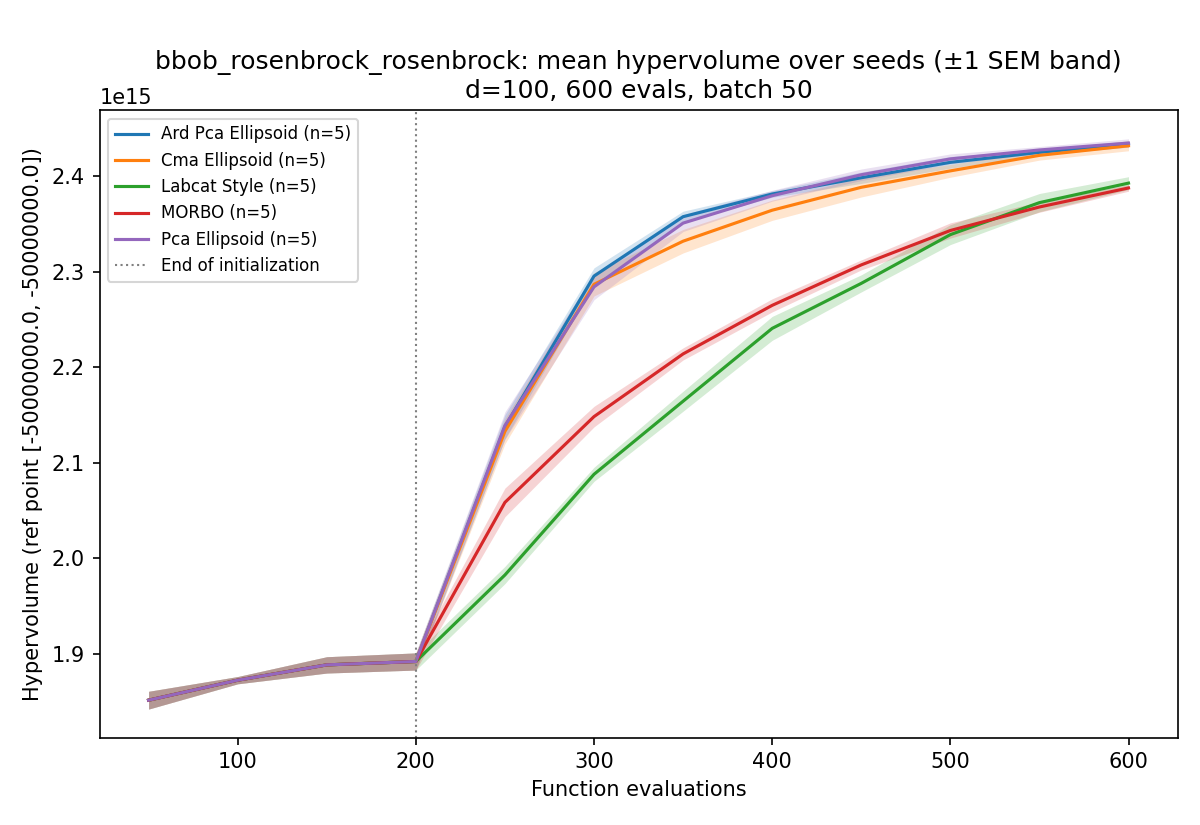
\includegraphics[width=0.85\textwidth]{bbob_rosenbrock_aggregate.png}
\caption{Mean hypervolume vs.\ evaluations,
\texttt{bbob\_rosenbrock\_rosenbrock} -- LABCAT's own reported win
condition. \texttt{ard\_pca\_ellipsoid}, \texttt{pca\_ellipsoid}, and
\texttt{cma\_ellipsoid} separate early and stay ahead;
\texttt{labcat\_style} instead tracks isotropic \texttt{morbo} closely for
most of the run.}
\label{fig:bbob-rosenbrock}
\end{figure}

The sharpest single result is a failure mode at
$d{=}150$: raw final hypervolumes collapse to exactly $0.0$ in 3 of 5
seeds (\texttt{morbo}'s own well-documented failure signature there),
while both our PCA variants maintain a healthy $\approx 20$--$29$ in every
seed -- whitening by a noisy per-dimension lengthscale estimate
\emph{before} eigendecomposing appears to make the resulting rotation
itself more fragile as $d$ grows than \texttt{ard\_pca\_ellipsoid}'s
"PCA first, reweight fixed axes afterward" ordering. Aggregated across all
42 experiments, \texttt{labcat\_style} loses wherever a real signal
exists (the DTLZ2 sweep, DTLZ3/5/7, the informative non-stationary regime,
all 8 BBOB pairs) and roughly ties our methods where nothing helps anyone
(LassoBench, SparseRover, the near-null effective-dimension regimes) --
consistent with, not contradicting, the effective-dimension theory
(\S\ref{sec:tr-shape-summary}). One exception favors \texttt{labcat\_style}:
it beats \texttt{cma\_ellipsoid} on \texttt{tr\_shape\_methods\_dtlz2\_100d}
by $+19.5\%$, though the $n{=}5$ CI still touches zero. Two confounds
temper how far this generalizes to LABCAT's own single-objective setting:
our multi-objective weighting substitution may be a genuinely weaker
signal than LABCAT's own single-scalar ranking, and LABCAT's construction
was tuned and evaluated in a lower-dimensional single-objective regime,
so the $d{=}150$ collapse may reflect a scaling limit specific to this
study's regime rather than a flaw in LABCAT as originally scoped. What the
ablation \emph{does} establish cleanly: our own ordering choice is the
empirically more robust construction in the multi-objective,
high-dimensional regime this study targets, not merely the one that
avoids the degenerate no-op. Full numbers and per-experiment breakdown:
RESULTS.md \S13.

\begin{figure}[h]
\centering
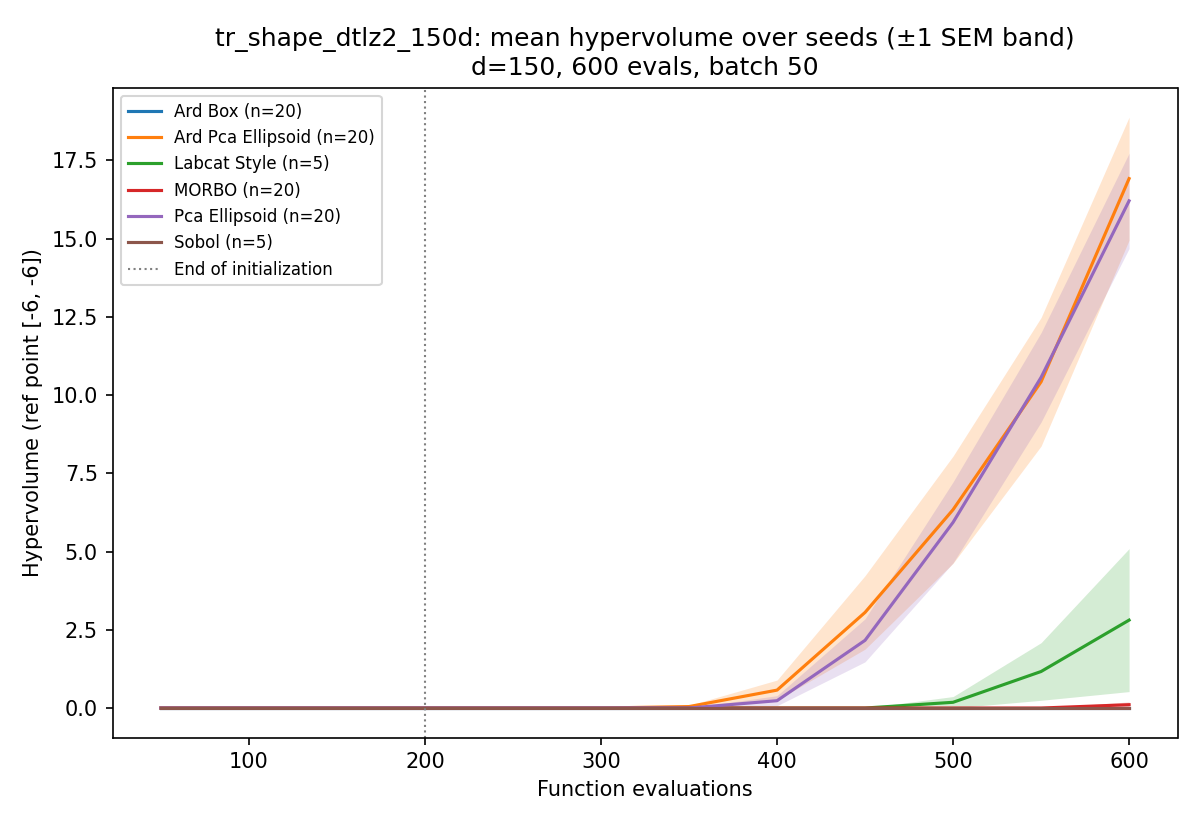
\includegraphics[width=0.85\textwidth]{dtlz2_150d_labcat_collapse.png}
\caption{Mean hypervolume vs.\ evaluations, $d{=}150$ DTLZ2. Both PCA
variants break through cleanly; \texttt{labcat\_style} tracks isotropic
\texttt{morbo} near zero through most of the budget and only barely
separates late, with a SEM band wide enough to include zero for most of
the run -- the collapse described above, visualized.}
\label{fig:dtlz2-150d-labcat-collapse}
\end{figure}

\subsection{\texttt{cma\_turbo\_style}: replicating CMA-TuRBO's own mechanism}
\label{sec:cma-turbo-style}

\S\ref{sec:tr-shape}'s "Relation to prior work" identifies CMA-BO/CMA-TuRBO
\citep{ngo2024cmabo} as mechanistically closer to \texttt{cma\_ellipsoid}
than an abstract-level read suggests, once the paper's actual construction
(verified directly from its PDF, not summarized from the abstract) is laid
out precisely. Two genuine mechanistic differences from
\texttt{cma\_ellipsoid}, both taken directly from the source paper's own
equations:

\begin{enumerate}
\item \textbf{Candidate sampling.} CMA-TuRBO draws candidates by direct
multivariate-Gaussian sampling from the adapted covariance,
$N(m, L^2\Sigma)$, rejecting and resampling any draw outside a
$\chi^2_{1-\alpha,d}$-radius confidence ellipsoid (verified against the
reference implementation, github.com/LamNgo1/cma-meta-algorithm -- the
paper's own "3-sigma rule" is a fixed \emph{label} for a radius that
actually scales with dimension via the chi-squared quantile, not a
literal ``3'' at any $d>1$) -- not the rotated-box perturbation every other
method in this section uses. \texttt{cma\_turbo\_style} implements this
directly (\texttt{sample\_tr\_gaussian\_ellipsoid}, morbo/utils.py):
candidates are drawn from
$N(x_c, R\,\mathrm{diag}((a/(2r))^2)\,R^\top)$ with
$r=\sqrt{\chi^2_{0.9973,d}}$, interpreting $a/2$ (this project's own
axis-width convention) as the extent along that dimension-correct radius,
with the same reject-and-resample step as the reference code.
\item \textbf{Covariance update.} CMA-TuRBO's rank-$\mu$ update uses
\emph{unmodified CMA-ES}: the best $\mu = \lfloor n/2 \rfloor$ of ALL local
points (not just Pareto-elites), weighted by classical log-rank weights
$w_i = \log(\mu+0.5) - \log(i)$ for rank $i=1,\ldots,\mu$ (normalized to
sum to 1) rather than equally. \texttt{cma\_turbo\_style} implements this
directly (\texttt{compute\_cma\_turbo\_style\_shape}, morbo/utils.py),
reusing \texttt{cma\_ellipsoid}'s persistent covariance/evolution-path
state (only one CMA-style mode is ever active per trust region) and
otherwise identical in structure -- same blending coefficients, same
rank-one evolution-path term -- so the ablation isolates exactly the
ranking question, not every CMA-ES engineering detail (in particular,
neither this nor \texttt{cma\_ellipsoid} implements ``active'' CMA's
negative weights for the worst points).
\end{enumerate}

\textbf{Disclosed simplifications.} Trust-region \emph{containment} (which
existing points count as local, via the same machinery every other mode
uses) still uses the L-infinity rotated box, not CMA-TuRBO's own
Mahalanobis/L2 ellipsoid test -- only candidate \emph{sampling} changes.
CMA-TuRBO's rank-$\mu$ update draws on a fresh $\lambda$-sized population
each CMA "generation" (an outer loop wrapping a full TuRBO sub-run);
\texttt{cma\_turbo\_style} instead ranks the trust region's own
accumulated local data at each per-iteration refit, the same cadence every
other mode in this study uses -- introducing a second, CMA-generational
timescale into MORBO's iteration structure was judged not worth the
implementation risk for what this ablation needs to test.
\textbf{Multi-objective adaptation}: the source paper ranks its population
by literal fitness value; with no single scalar to rank by, points are
ranked by the mean of their per-objective values, independently min-max
normalized across the local population (higher is better) -- the same
substitution already established for \texttt{labcat\_style}, not a new one
invented here.

Run against \texttt{cma\_ellipsoid} on the core comparison
(\texttt{tr\_shape\_dtlz2\_100d}, \texttt{tr\_shape\_methods\_dtlz2\_100d})
and \texttt{cma\_ellipsoid}'s own strongest documented landscapes
(\texttt{RotatedSparseDTLZ2} at $k_{\mathrm{eff}}{=}50$, where
\texttt{cma\_ellipsoid} is the only unanimous winner under a rotated
effective subspace, and \texttt{bbob\_rosenbrock\_rosenbrock}), 5 seeds
each (\texttt{cluster/submit\_cma\_turbo\_style.sh}, 20 jobs). Results
queued; see RESULTS.md \S15.

\subsection{Consuming the shape: sampling and containment}

Both new operations are rotated-frame analogues of MORBO's existing
isotropic primitives, and reduce to them exactly when $R=I$. Containment
(\texttt{get\_indices\_in\_ellipsoid}, used for center selection and
candidate-pool filtering) tests $|w_k| \le a_k/2\ \forall k$ in the rotated
frame $w = (x-x_c)R$, in place of the isotropic $|x_k - x_{c,k}| \le
\ell/2$. Candidate sampling
(\texttt{sample\_tr\_discrete\_points\_subset\_d\_rotated}) mirrors
MORBO's existing subset-perturbation scheme -- perturbing only
$\lceil d \cdot \min(20/d, 1)\rceil$ of the $d$ available directions per
candidate, bounding simultaneous degrees of freedom in high dimension --
but crucially performs that masking \emph{in the rotated basis}, on $w$
rather than on the original coordinates: masking raw dimensions and
rotating afterward would smear a single "masked-in" raw direction across
every principal axis post-rotation, defeating the point of a sparse
perturbation entirely. One notable exclusion: \texttt{trunc\_normal\_perturb}
is not supported together with a non-isotropic \texttt{tr\_shape} (an
explicit error, not a silent fallback to unrotated behavior).

One deliberate asymmetry: \emph{trust-region data selection}
(\texttt{trim\_trace}, which points the local GP is fit on) is
\textbf{not} routed through the shaped containment test, regardless of
\texttt{tr\_shape} -- it always uses the isotropic box. Since GP fitting's
own input normalization stays isotropic (Section~\ref{sec:tr-shape}'s first
paragraph), selecting training data from an eccentric rotated region here
would feed values that are badly out-of-range in one direction and crushed
near zero in another into that fixed isotropic normalization, undermining
the very invariant ("GP fitting is unaffected by \texttt{tr\_shape}") the
scoping decision above was meant to guarantee.

\begin{table}[h]
\centering
\caption{Trust-region shape adaptation, DTLZ2 direct modeling, dimension
sweep at fixed budget (600 evals, batch 50, 3 trust regions), now over 5
seeds (0--4). Percentages are mean paired per-seed deltas relative to the
isotropic \texttt{morbo} baseline at the same seed and $d$; win-rate is the
fraction of seeds where the variant beats baseline. At $d=150$ the
baseline is $\approx 0$ for 4/5 seeds, so absolute hypervolume deltas are
reported instead of percentages.}
\label{tab:tr-shape-sweep}
\begin{tabular}{lrrrr}
\toprule
$d$ & \texttt{morbo} (mean$\pm$std) & \texttt{ard\_box} & \texttt{pca\_ellipsoid} & \texttt{ard\_pca\_ellipsoid} \\
\midrule
50  & $32.93\pm0.35$ & $-4.0\%$ (0/5) & $+3.3\%$ (5/5) & $+4.1\%$ (5/5) \\
100 & $19.90\pm0.91$ & $-49.2\%$ (0/5) & $+66.6\%$ (5/5) & $+66.4\%$ (5/5) \\
150 & $0.08\pm0.17$\textsuperscript{\dag} & $+0.00$ (0/5) & $+20.3$\textsuperscript{\dag} (5/5) & $+23.0$\textsuperscript{\dag} (5/5) \\
\bottomrule
\end{tabular}

\vspace{0.5em}
\footnotesize\textsuperscript{\dag}Absolute hypervolume, not a percentage:
the isotropic baseline is $\approx 0$ at this $d$ for 4/5 seeds, so no ratio
is defined for most seeds.
\end{table}

\begin{figure}[h]
\centering
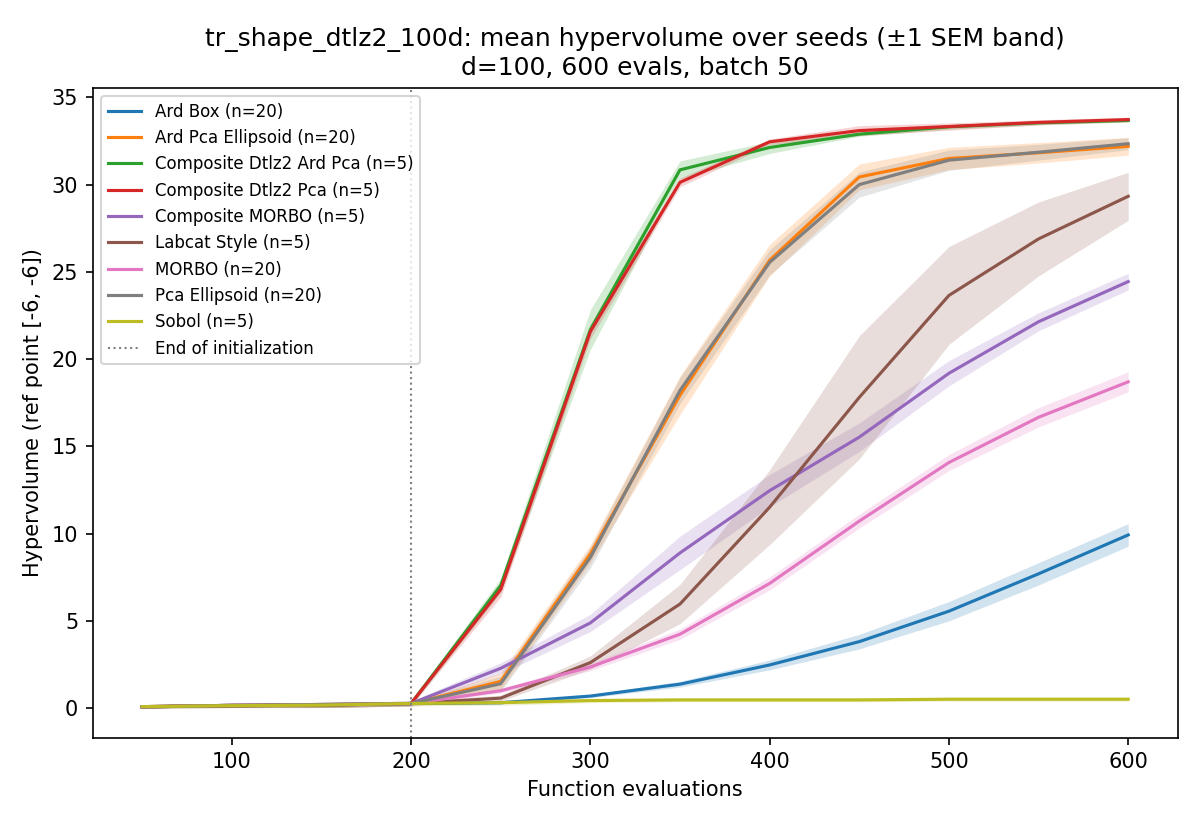
\includegraphics[width=0.85\textwidth]{dtlz2_100d_aggregate.png}
\caption{Mean hypervolume vs.\ evaluations, $d{=}100$ DTLZ2, $\pm 1$ SEM
band ($n$ per curve in the legend). The two PCA variants
(\texttt{pca\_ellipsoid}, \texttt{ard\_pca\_ellipsoid}) and their composite
counterparts (\S\ref{sec:composite}) separate cleanly and early from
isotropic \texttt{morbo}; \texttt{ard\_box} trails even the isotropic
baseline (\S\ref{sec:tr-shape}'s constraint-compounding diagnosis).
\texttt{labcat\_style} (\S\ref{sec:labcat-style}) lands between the two
groups -- clearly better than isotropic, clearly behind our own PCA
variants.}
\label{fig:dtlz2-100d-aggregate}
\end{figure}

\subsection{Results: a curse-of-dimensionality effect, diagnosed directly, and confirmed unanimous across seeds}

Table~\ref{tab:tr-shape-sweep} shows the same three-regime pattern as the
original single-seed sweep, now with every seed agreeing on direction. At
$d=50$ and $d=100$ the win/loss pattern is \textbf{unanimous across all 5
seeds}: \texttt{ard\_box} loses in $5/5$, both PCA variants win in $5/5$,
with non-overlapping ranges (at $d=100$, \texttt{ard\_box}'s best seed is
still a $-34.6\%$ loss; \texttt{pca\_ellipsoid}'s worst seed is still a
$+56.5\%$ win). At $d=150$, \texttt{ard\_box} is \emph{exactly} $0.00$ on
all 5 seeds, matching the baseline's failure exactly, while both PCA
variants break through on all 5. This is as strong as a 5-seed result can
be -- not a lucky single draw, but a systematic, seed-independent effect.
\texttt{ard\_box}'s failure also grows more variable with $d$ (std
$0.79 \to 2.58$ from $d{=}50$ to $d{=}100$) even as its mean loss grows,
consistent with the per-dimension lengthscale-collapse mechanism
(Section below) being present at every seed but variable in severity.

As an independent negative control at low dimension with a real,
non-synthetic problem, a $d=7$, $M=3$ Penicillin fermentation benchmark
(direct modeling, Section~\ref{sec:penicillin}'s simulator) shows all three
variants within $\pm 7\%$ of baseline -- consistent with the effect being
specific to high $d$, not problem type or objective count.

\paragraph{Why \texttt{ard\_box} fails, diagnosed directly.} A single GP
fit on synthetic $d=100$ local data (200 points, no full BO loop needed)
gives fitted lengthscales spanning a $15.2\times$ ratio ($\min=0.26$,
$\max$ at the constraint ceiling of $4.0$ -- correctly identifying $\sim
99$ of $100$ dimensions as smooth/uninformative and one as sharply
informative). Equation~\ref{eq:ard-box} applies this literally: of the same
$200$ local points, only \textbf{$1$} falls inside the resulting
\texttt{ard\_box} region, versus \textbf{$41$} for \texttt{pca\_ellipsoid}'s
data-covariance-derived shape on identical data ($5.7\times$ axis ratio).
Containment requires satisfying $d$ independent per-axis constraints
\emph{simultaneously} (a logical AND, not an OR); even though total volume
is preserved exactly ($\prod_k a_k = \ell^d$ by construction), the
intersection of $100$ independent narrowed constraints collapses
combinatorially once real data isn't spread uniformly through that volume
-- which it never is. This is precisely why \texttt{ard\_box} underperforms
even the isotropic baseline that ignores lengthscale information entirely:
using more information hurts once that information is applied as $d$
separate hard constraints rather than a single shared one, since any
per-dimension estimation noise (lengthscale estimates are themselves
uncertain early in optimization, with limited data spread across $d$ axes)
gets baked into the geometry and compounds with every other dimension's
constraint. \texttt{pca\_ellipsoid}/\texttt{ard\_pca\_ellipsoid} avoid this
because their shape comes from the correlation structure of actually
\emph{collected} data -- a genuine lower-dimensional effective subspace --
rather than $d$ independently-estimated per-axis hyperparameters treated as
separate constraints.

This same mechanism produced a real (if unrelated-looking) bug during
testing: on the Rover benchmark ($d=60$, a real navigation problem whose
raw parameters get cumulatively summed into spline control points, see
\texttt{morbo/problems/rover.py}), one collapsed axis width
($a_k = 0.019$ against $a_j \approx 0.85$ for the rest, a $45\times$ gap)
produced near-duplicate consecutive spline control points, crashing
\texttt{scipy}'s exact-interpolation cubic fit outright rather than merely
degrading hypervolume -- the same collapse, just manifesting as a hard
numerical failure instead of a quiet performance loss, in a benchmark whose
evaluator happens to be fragile to near-duplicate inputs. Fixed by treating
such evaluation failures as a large finite penalty rather than crashing the
run, since the underlying candidate collapse is an expected consequence of
this method's own geometry, not a bug in the sampler that produced it.

\subsection{Extended budget at $d=200$: breakthrough, not failure}

The all-zero $d=200$ row of Table~\ref{tab:tr-shape-sweep} is a budget
effect, not a method failure. Rerunning $d=200$ at $2000$ evaluations
(everything else identical) shows every method eventually finding
reference-point-dominating solutions -- in exactly the same ranking as
$d=100$ and $d=150$:

\begin{table}[h]
\centering
\caption{Extended-budget follow-up: DTLZ2, $d=200$, 2000 evals, batch 50,
seed 0. "Breakthrough" is the evaluation at which true hypervolume first
exceeds zero.}
\label{tab:tr-shape-200d-2000ev}
\begin{tabular}{lrrr}
\toprule
Method & Final HV & vs.\ baseline & Breakthrough \\
\midrule
\texttt{morbo} (isotropic) & 19.32 & --- & $\sim$1150 \\
\texttt{ard\_box} & 14.81 & $-23.4\%$ & $\sim$1450 \\
\texttt{pca\_ellipsoid} & 28.79 & $+49.0\%$ & $\sim$800 \\
\texttt{ard\_pca\_ellipsoid} & \textbf{33.15} & $\mathbf{+71.6\%}$ & $\sim$750 \\
\bottomrule
\end{tabular}
\end{table}

The PCA variants break through $\sim$400 evaluations before the isotropic
baseline and $\sim$700 before \texttt{ard\_box}, and convert that head
start into a large final gap. Notably, \texttt{ard\_pca\_ellipsoid}'s
final 33.15 at $d=200$ nearly matches what the isotropic baseline achieves
at $d=20$ (34.91) -- an order of magnitude more nominal dimensions at
almost no hypervolume cost.

\subsection{A real-problem check that sharpens the claim: Rover (corrected with 5 seeds)}

An earlier single-seed run of Rover ($d=60$, $M=2$) reported that
\emph{no} shape variant beat the isotropic baseline, with
\texttt{pca\_ellipsoid} -- the DTLZ2 sweep's strongest method -- doing
\emph{worst} of the three. Rerunning across 5 seeds shows that single-seed
result was \textbf{noise, not signal}: that seed happened to be
\texttt{pca\_ellipsoid}'s worst of the five.

\begin{table}[h]
\centering
\caption{Rover ($d=60$, $M=2$), 5 seeds. Win-rate is paired per-seed wins
against \texttt{morbo} at the same seed; mean \% is the mean paired delta.}
\label{tab:tr-shape-rover}
\begin{tabular}{lrrr}
\toprule
Method & Mean HV & Win-rate & Mean paired \% \\
\midrule
\texttt{morbo} & $2.20\pm0.14$ & --- & --- \\
\texttt{ard\_box} & $2.15\pm0.24$ & 2/5 & $-1.8\%$ \\
\texttt{pca\_ellipsoid} & $2.30\pm0.12$ & 3/5 & $\mathbf{+4.9\%}$ \\
\texttt{ard\_pca\_ellipsoid} & $2.24\pm0.22$ & 2/5 & $+1.4\%$ \\
\bottomrule
\end{tabular}
\end{table}

Averaged over 5 seeds, \texttt{pca\_ellipsoid}'s mean is actually
\emph{above} baseline ($+4.9\%$), and all three variants show win-rates
near a coin flip ($2/5$, $3/5$, $2/5$) with per-seed swings ($\pm10$--$23\%$)
far larger than any mean effect -- the opposite of DTLZ2's unanimous
$5/5$-or-$0/5$ pattern (Table~\ref{tab:tr-shape-sweep}).

This sharpens, rather than weakens, the core claim. DTLZ2's effective
structure is extremely low-dimensional: one informative position variable,
with the remaining $d-1$ entering only through the smooth scalar $g(x)$ --
precisely the structure a PCA rotation can discover and align with, and
every seed agrees. Rover's 60 spline-waypoint coordinates all matter
roughly equally -- there is no low-dimensional effective subspace to find
-- so the rotation's effect is dominated by covariance-estimation noise (a
$60\times60$ matrix estimated from limited local data), producing an effect
that \emph{flips sign from seed to seed} rather than one that is
consistently mildly harmful. The refined claim is therefore
\textbf{conditional and now evidenced by contrast in variance, not just in
mean}: trust-region shape adaptation produces a systematic, seed-robust
effect when the problem has low-dimensional effective structure to align
with, and produces a noise-level, seed-flipping effect when it doesn't. The
$d=7$ Penicillin negative control (all variants within $\pm7\%$ of
baseline, single seed) is consistent with the low-effective-structure side
of this claim.

\subsection{New shape mechanisms: CMA-ES covariance adaptation, a linear-kernel baseline, and a dimension-scaled lengthscale prior}

Motivated by two papers read after the sweep above --
\citet{wang2026assmea} (surrogate-assisted evolutionary local-region search,
"AS-SMEA") and \citet{doumont2026linearbo} ("We Still Don't Understand
High-Dimensional Bayesian Optimization") -- three further mechanisms were
implemented and run at $d\in\{100,150,200\}$ (single seed; see
\texttt{writeup/FURTHER\_DIRECTIONS.md} for full motivation).

\paragraph{\texttt{cma\_ellipsoid}.} Rather than recomputing $R$/$a$ from
scratch each iteration (as \texttt{pca\_ellipsoid} does), this variant
maintains a persistent per-trust-region covariance $C$, updated each
iteration by a CMA-ES-style rank-$\mu$-plus-rank-1 rule from the region's
Pareto elites and an evolution path:
\begin{equation}
  C^{(t)} = (1-c_1-c_\mu)\,C^{(t-1)} + c_\mu \sum_i w_i (x_i-m)(x_i-m)^\top + c_1\,p\,p^\top,
\end{equation}
with $R$/$a$ obtained by eigendecomposing $C^{(t)}$ each iteration exactly
as for \texttt{pca\_ellipsoid}. This makes shape adaptation temporally
smoothed and incremental rather than memoryless.

\paragraph{\texttt{linear\_gp} (\texttt{\_pca}/\texttt{\_cma}).} A
spherically-projected linear-kernel GP (\citealp{doumont2026linearbo}'s
proposed fix to the linear kernel's boundary-seeking pathology): the
$[0,1]^d$ cube is bijectively mapped onto the upper hypersphere in
$\mathbb{R}^{d+1}$ before a \texttt{LinearKernel}, tested alone and crossed
with \texttt{pca\_ellipsoid}/\texttt{cma\_ellipsoid} shape.

\paragraph{\texttt{ard\_box\_dimprior}/\texttt{ard\_pca\_dimprior}.} A
dimension-scaled LogNormal lengthscale prior (\citealp{hvarfner2024vanilla})
in place of the hard \texttt{Interval(0.05, 4.0)} constraint, as a candidate
fix for \texttt{ard\_box}'s diagnosed collapse (Section above): if the
collapse were caused by lengthscales pinning against the interval's
ceiling, a prior with no ceiling that expects $\lambda \sim \sqrt{d}$ should
relieve it.

\begin{table}[h]
\centering
\caption{New shape mechanisms vs.\ established methods, DTLZ2, single seed.
Baseline (\texttt{morbo}) is $20.02$ at $d{=}100$ and $0.00$ at
$d{\in}\{150,200\}$ within the standard 600-eval budget.}
\label{tab:tr-shape-new-methods}
\begin{tabular}{lrrr}
\toprule
Method & $d{=}100$ & $d{=}150$ & $d{=}200$ \\
\midrule
\texttt{ard\_box\_dimprior} & 11.07 & --- & 0.00 \\
\texttt{ard\_pca\_dimprior} & 32.83 & 18.17 & 0.00 \\
\texttt{cma\_ellipsoid} & 24.29 & 26.99 & \textbf{21.72} \\
\texttt{linear\_gp} & 15.91 & 0.00 & 0.00 \\
\texttt{linear\_gp\_cma} & 21.41 & --- & --- \\
\texttt{linear\_gp\_pca} & \textbf{33.34} & 28.02 & 0.00 \\
\bottomrule
\end{tabular}
\end{table}

\textbf{Headline finding: \texttt{cma\_ellipsoid} is the only method of nine
tested -- including every PCA variant and every linear-kernel combination --
that breaks through at $d{=}200$ within the standard 600-eval budget.} This
directly validates the AS-SMEA-motivated design: CMA's covariance is a
persistent state that begins adapting from the first iteration, whereas the
PCA variants recompute their shape from scratch each iteration and need
enough accumulated local data for a reliable eigendecomposition -- a
requirement that gets harder to satisfy exactly when $d$ is large relative
to the eval budget. This is the regime in which temporal smoothing
(AS-SMEA's core design argument) actually matters, rather than being a
theoretical nicety.

Two negative results are also informative. First, \textbf{the
dimension-scaled prior does not fix \texttt{ard\_box}}: removing the hard
ceiling makes it \emph{worse} ($11.07$ vs.\ plain \texttt{ard\_box}'s
$13.09$ at the same scale), consistent with the diagnosed mechanism being
structural (treating $d$ independent lengthscale estimates as $d$ separate
hard constraints) rather than about where those lengthscales numerically
sit -- a soft, uncapped prior can make the per-axis spread \emph{more}
extreme, not less. Second, \textbf{kernel choice matters far less than
trust-region shape}: \texttt{linear\_gp} alone is clearly worse than
Mat\'ern ($-20.5\%$ at $d{=}100$), but paired with PCA shape it fully
recovers, matching the best Mat\'ern+PCA result at both $d{=}100$ and
$d{=}150$ -- though this recovery does not extend to $d{=}200$, where
\texttt{linear\_gp\_pca} fails along with every other PCA-based method.
This suggests PCA-based shape adaptation does most of the work of finding
a problem's effective low-dimensional structure, with the surrogate model
riding on top of an already well-shaped search region.

\subsection{Composite modeling $\times$ shape adaptation: an approximately additive interaction}

Since composite modeling changes \emph{what} the surrogate models while
shape adaptation changes only \emph{how} candidates are sampled around
whatever the surrogate predicts, the two extensions built in this work
should compose without new code -- verified directly on Penicillin
($d{=}7$, $M{=}3$) as a $2\times2$: \{direct, composite\} $\times$
\{isotropic, PCA-shaped\}, plus \texttt{ard\_pca\_ellipsoid} as a fifth arm.

\begin{table}[h]
\centering
\caption{Composite $\times$ shape, Penicillin, single seed, one cluster run
(values are directly comparable to each other but not to
Table~\ref{tab:penicillin-results}'s CPU-run baseline; see text).}
\label{tab:tr-shape-composite-2x2}
\begin{tabular}{lrr}
\toprule
Cell & Final HV & vs.\ this run's \texttt{morbo} \\
\midrule
Direct + isotropic (\texttt{morbo}) & 373082.3 & --- \\
Direct + PCA & 347228.2 & $-6.9\%$ \\
Composite + isotropic & 369704.6 & $-0.9\%$ \\
Composite + PCA & 360577.4 & $-3.4\%$ \\
Composite + ARD-PCA & 347985.4 & $-6.7\%$ \\
\bottomrule
\end{tabular}
\end{table}

This run's \texttt{morbo} baseline ($373082.3$) does not numerically match
the original composite-Penicillin experiment's \texttt{morbo}
($347702.9$) at the nominally identical seed and config -- attributed to
CPU-vs-GPU/BLAS floating-point non-determinism (the original was a laptop
CPU run; this is a cluster GPU run), not a bug, so comparisons here are
restricted to \emph{within this run}, where all five cells share the same
environment. Composite modeling alone is roughly neutral in this run
($-0.9\%$), shape adaptation alone costs about $-7\%$ (consistent with
Penicillin's low-$d$ negative-control role elsewhere), and combined the
cost is roughly additive ($-3.4\%$ to $-6.7\%$) rather than amplified or
cancelled -- consistent with the two extensions touching disjoint parts of
the pipeline, and with Section above's finding that shape adaptation has no
systematic effect at Penicillin's scale in the first place.

\subsection{\texttt{mab\_shape}: adaptive shape selection wins where there is time to learn, and loses where there isn't}

Since no single fixed shape wins on every problem tested (PCA wins on
DTLZ2, no shape robustly wins on Rover), a natural next step -- AS-SMEA's
own answer to the same problem (Wang et al. 2026, Sec.\ 3.3, their
LS-IMA/MASS) -- is to let each trust region \emph{learn} which shape suits
its own local landscape rather than fixing one globally. \texttt{tr\_shape
= "mab\_shape"} implements this as a per-trust-region epsilon-greedy
bandit over $\{$\texttt{isotropic}, \texttt{ard\_box}, \texttt{pca\_ellipsoid},
\texttt{ard\_pca\_ellipsoid}, \texttt{cma\_ellipsoid}$\}$, re-selected each
time the local model refits; reward is binary (1.0 if the TR's own success
streak was just incremented, else 0.0), folded into a per-arm exponential
moving average.

\begin{table}[h]
\centering
\caption{\texttt{mab\_shape} vs.\ the best fixed shape at each $d$, standard
600-eval budget (DTLZ2, single seed; Rover single seed, not directly
comparable to the 5-seed means elsewhere in this section). The $d{=}150$/$200$
zeros are resolved below as a budget artifact, not a standing failure.}
\label{tab:tr-shape-mab}
\begin{tabular}{lrrl}
\toprule
Problem & \texttt{morbo} & \texttt{mab\_shape} & vs.\ best fixed shape here \\
\midrule
DTLZ2 $d{=}100$ & 20.02 & \textbf{33.89} ($+69.2\%$) & best of all 8 methods tested \\
DTLZ2 $d{=}150$ & 0.00 & 0.00 & pca/cma/linear\_gp\_pca all break through (27--29) \\
DTLZ2 $d{=}200$ & 0.00 & 0.00 & only \texttt{cma\_ellipsoid} (21.72) breaks through \\
Rover (seed 0) & 2.36 & 2.19 & within the near-coin-flip range of \S\ref{sec:tr-shape}'s fixed shapes \\
\bottomrule
\end{tabular}
\end{table}

This is a genuinely two-sided result. At $d{=}100$, \texttt{mab\_shape} is
the single best method of all eight tested in this section -- beating
every fixed shape it chooses among, plausibly by hedging early exploration
against a bad initial draw while still exploiting the winning arms once
identified. (\emph{Revised by the 20-seed program},
\S\ref{sec:twenty-seed}: that single-seed showing was a favorable draw --
at 20 seeds \texttt{mab\_shape} averages $+33.5\%$ with 15/20 wins but
std $7.2$, well below \texttt{linear\_gp\_pca} and the PCA variants.) But at $d{=}150$--$200$, where even the strongest fixed shapes
only barely break through late in a tight 600-eval budget
(breakthrough evals $\sim$300--350 of 600 for the PCA variants at
$d{=}150$), \texttt{mab\_shape} ties the \emph{failing} isotropic baseline
rather than approaching the winning fixed shapes: the bandit's own
exploration cost (a fixed $15\%$ of iterations, by default, spent on arms
that include the two actively harmful ones) consumes exactly the margin
the fixed-shape methods needed. The mechanism is a direct consequence of
the narrow, late-arriving breakthrough window diagnosed in
\S\ref{sec:tr-shape}: adaptivity's own learning cost becomes a net
negative exactly where the reward signal is scarcest.

\paragraph{Resolved: the $d{=}150$--$200$ failure was a pure budget
artifact.} Rerunning \texttt{mab\_shape} at the same 2000-eval budget used
for Table~\ref{tab:tr-shape-200d-2000ev}'s extended-$d{=}200$ follow-up
settles the question directly:

\begin{table}[h]
\centering
\caption{\texttt{mab\_shape} at extended budget (2000 evals), vs.\ the
established fixed-shape methods at the same budget. Percentages relative
to \texttt{morbo} at the same $d$.}
\label{tab:tr-shape-mab-2000ev}
\begin{tabular}{lrrrr}
\toprule
$d$ & \texttt{morbo} & \texttt{pca\_ellipsoid} & \texttt{ard\_pca\_ellipsoid} & \texttt{mab\_shape} \\
\midrule
150 & 25.95 & 29.23 ($+12.6\%$) & \textbf{34.26 ($+32.1\%$)} & 32.32 ($+24.6\%$) \\
200 & 19.32 & 28.79 ($+49.0\%$) & 33.15 ($+71.6\%$) & \textbf{33.61 ($+73.9\%$)} \\
\bottomrule
\end{tabular}
\end{table}

\texttt{mab\_shape} fully recovers given enough budget -- and at $d{=}200$
it becomes the single best method of every fixed-and-adaptive shape tested
anywhere in this study, edging out \texttt{ard\_pca\_ellipsoid} (previously
the strongest method at this scale). At $d{=}150$ it is a strong second
place, comfortably ahead of plain \texttt{pca\_ellipsoid} and the baseline,
just behind \texttt{ard\_pca\_ellipsoid}. This confirms the
$d{=}150$--$200$/600-eval failure was the same kind of budget artifact as
the isotropic baseline's own $d{=}200$/600-eval zero (Table~\ref{tab:tr-shape-200d-2000ev})
-- not a standing design flaw. The bandit's exploration cost is real (it is
why \texttt{mab\_shape} needed the extra budget the pre-converged fixed
shapes at $d{=}100$ did not), but it amortizes rather than compounding
indefinitely: once there is enough budget to pay the exploration tax
\emph{and} still exploit the learned arm, adaptivity's core promise -- not
needing to know the best fixed shape in advance -- pays off outright. A
budget-aware or annealed exploration rate remains worth trying as an
efficiency improvement (it should let \texttt{mab\_shape} reach the same
endpoint with less wasted exploration, potentially narrowing the
tight-budget $d{=}150$--$200$/600-eval gap too), but is no longer needed to
explain the earlier failure.

\subsection{\texttt{SparseDTLZ2}: effective dimension, not nominal dimension, governs the effect}
\label{sec:sparse-dtlz2}

Plain DTLZ2 confounds nominal and effective dimension: its
$k = d - M + 1$ distance dimensions all contribute to $g(x)$, so effective
dimensionality necessarily grows with nominal $d$. A new test problem,
\texttt{SparseDTLZ2} (\texttt{morbo/problems/sparse\_dtlz2.py}), breaks
this confound by masking all but \texttt{k\_eff} of the $k$ distance
dimensions out of $g(x)$ entirely -- the masked dimensions are literal
no-ops on every objective, not merely less informative -- so nominal and
effective dimension can be scaled independently. Two single-seed sweeps
(400 evals, batch 40, 3 TRs, smaller budget than the main sweep since
effective dimensionality is small by construction at every point tested):

\begin{table}[h]
\centering
\caption{Group A: nominal $d$ scaled $60 \to 200$ with effective dimension
pinned at $(M{-}1)+k_{\mathrm{eff}} = 6$. Percentages are relative to
\texttt{morbo} at the same nominal $d$.}
\label{tab:sparse-dtlz2-groupA}
\begin{tabular}{lrrr}
\toprule
Nominal $d$ & \texttt{pca\_ellipsoid} & \texttt{ard\_pca\_ellipsoid} & \texttt{cma\_ellipsoid} \\
\midrule
60  & $+0.19\%$ & $+0.18\%$ & $+0.30\%$ \\
80  & $+0.07\%$ & $+0.09\%$ & $+0.10\%$ \\
100 & $+0.13\%$ & $+0.17\%$ & $+0.22\%$ \\
150 & $+0.05\%$ & $+0.01\%$ & $+0.18\%$ \\
200 & $+0.05\%$ & $+0.03\%$ & $+0.13\%$ \\
\bottomrule
\end{tabular}
\end{table}

Flat and essentially null across a $60 \to 200$ nominal-dimension range --
every value is within $0.3\%$ of baseline, an order of magnitude below
even the smallest real effect seen anywhere else in this study. Scaling
nominal dimension alone, with effective dimension pinned small, produces
no method-dependent effect at all. This directly refutes a "gap between
nominal and effective dimension" framing considered earlier in this
project: nominal dimension is not, by itself, what shape adaptation
responds to.

\begin{table}[h]
\centering
\caption{Group B: nominal $d{=}100$ fixed, effective dimension scaled via
$k_{\mathrm{eff}} \in \{2,10,20,50\}$ (effective dim $= 1+k_{\mathrm{eff}}$).
Percentages relative to \texttt{morbo} at the same $k_{\mathrm{eff}}$.}
\label{tab:sparse-dtlz2-groupB}
\begin{tabular}{lrrr}
\toprule
$k_{\mathrm{eff}}$ (effective dim) & \texttt{pca\_ellipsoid} & \texttt{ard\_pca\_ellipsoid} & \texttt{cma\_ellipsoid} \\
\midrule
2 (3)   & $+0.09\%$ & $+0.08\%$ & $+0.10\%$ \\
5 (6)   & $+0.13\%$ & $+0.17\%$ & $+0.22\%$ \\
10 (11) & $+0.06\%$ & $+0.05\%$ & $+0.24\%$ \\
20 (21) & $+1.02\%$ & $+0.57\%$ & $+0.97\%$ \\
50 (51) & $\mathbf{+6.7\%}$ & $-0.55\%$ & $\mathbf{+10.1\%}$ \\
\bottomrule
\end{tabular}
\end{table}

A clean, monotonic dose-response as effective dimension grows, with
nominal dimension held fixed the entire time: effect size grows smoothly
from noise level ($\sim$0.1\% at effective dim 3) through a first visible
signal ($\sim$1\% at effective dim 21) to a real effect ($+6.7$ to
$+10.1\%$ at effective dim 51) -- extrapolating cleanly toward the
$+64$--$67\%$ seen in Table~\ref{tab:tr-shape-sweep} at $d{=}100$
(effective dimension $\approx 99$, full 600-eval budget). Combined with
Group A's flat null, this pins down the mechanism precisely: it is
\textbf{effective dimension relative to the eval budget}, not nominal
dimension and not the gap between them, that determines when trust-region
shape adaptation starts to matter. The plain-DTLZ2 dimension sweep
(Table~\ref{tab:tr-shape-sweep}) was measuring effective dimension all
along -- nominal $d$ there was only ever a proxy for it, since DTLZ2's own
construction ties the two together.

One exception is worth flagging plainly: at effective dimension 51,
\texttt{ard\_pca\_ellipsoid} is the one method that does \emph{not} win
($-0.55\%$, the only negative value in either table), while plain
\texttt{pca\_ellipsoid} ($+6.7\%$) and \texttt{cma\_ellipsoid} ($+10.1\%$,
the strongest of the three here, consistent with \texttt{cma\_ellipsoid}'s
disproportionate strength in tight-budget/high-effective-dimension regimes
noted above) both win clearly. A plausible reading is that this is the
same lengthscale-noise-compounding mechanism diagnosed for
\texttt{ard\_box} above, partially reappearing in the ARD-reweighted
hybrid once there is enough real per-dimension signal (51 informative
axes) for early lengthscale estimates to be individually noisy within a
tighter, 400-eval budget -- a single-seed observation that warrants a
multi-seed follow-up before being treated as more than suggestive.

\subsection{\texttt{sobol}: is any of this machinery earning its keep?}

Every result above compares shape-adaptation variants against
\texttt{morbo} itself, which already assumes TuRBO's local trust-region
and GP-surrogate machinery is worth having in the first place.
\texttt{label="sobol"} tests that assumption directly: a single continuous
Sobol low-discrepancy sequence over the whole search space, no trust
regions or GP fitting at all, evaluated in matched batches.

\begin{table}[h]
\centering
\caption{\texttt{sobol} vs.\ \texttt{morbo}, 5 seeds where available (matching
Table~\ref{tab:tr-shape-sweep}/\S\ref{sec:tr-shape}'s Rover result).}
\label{tab:tr-shape-sobol}
\begin{tabular}{lrrl}
\toprule
$d$ / problem & \texttt{morbo} & \texttt{sobol} & vs.\ sobol \\
\midrule
50  & $32.93\pm0.35$ & $23.78\pm0.34$ & $+38.5\%$ \\
100 & $19.90\pm0.91$ & $0.51\pm0.25$ & $+3800\%$ (sobol barely clears the ref.\ point) \\
150 & $0.08\pm0.17$ & $0.00\pm0.00$ & both near zero at this budget \\
200 & $0.00$ & $0.00\pm0.00$ & both zero at this budget \\
Rover & $2.20\pm0.14$ & $1.26\pm0.09$ & $+74.6\%$ \\
\bottomrule
\end{tabular}
\end{table}

MORBO's local-modeling machinery earns its keep decisively, with the
margin growing sharply with dimension until both approaches run out of
budget together at $d{\ge}150$ (not a \texttt{sobol}-specific failure --
\emph{nothing} breaks through reliably there at this budget, per
\S\ref{sec:tr-shape}). At $d{=}100$ the gap is enormous: random search
barely clears the reference point at all ($0.51$) against \texttt{morbo}'s
$19.90$ and the best shaped variant's $33{+}$ -- roughly a $65\times$ gap
over \texttt{sobol}. On Rover, where shape adaptation itself showed no
robust effect (\S\ref{sec:tr-shape}), the underlying trust-region/GP
machinery still clearly beats random search ($+74.6\%$), confirming that
Rover's "no shape helps" result is specifically about \emph{geometry}, not
a sign that local modeling is worthless on that problem too. This is the
right context for every other result in this section: shape adaptation's
$+64$--$72\%$ wins sit on top of an already-large base advantage MORBO has
over random search, not the whole story on their own.

\subsection{Compute efficiency: hypervolume per unit of optimizer time}

Every saved run records per-iteration model-fitting and
candidate-generation wall-times, enabling a compute-efficiency view --
cumulative optimizer time vs.\ hypervolume reached -- that equal-evaluation
comparisons hide. (Optimizer overhead is the relevant compute cost on
synthetic problems, where evaluation itself is microseconds; on expensive
real problems evaluation cost dominates instead and per-evaluation
comparisons are the right lens. Wall-times are compared only within an
experiment, all run on identical B200-GPU nodes.)

\begin{table}[h]
\centering
\caption{Total optimizer wall-time (GP fitting + candidate generation) vs.\
final hypervolume, seed 0. "Best shaped" is \texttt{ard\_pca\_ellipsoid}
except at $d{=}200$/2000ev where \texttt{mab\_shape} (503s $\to$ 33.6) also
exceeds it.}
\label{tab:tr-shape-efficiency}
\begin{tabular}{lrr}
\toprule
Experiment & \texttt{morbo} & best shaped variant \\
\midrule
$d{=}50$ & 93s $\to$ 32.7 & 87s $\to$ 34.2 \\
$d{=}100$ & \textbf{1505s} $\to$ 20.0 & 133s $\to$ 33.4 \\
$d{=}150$ & 96s $\to$ 0.0 & 108s $\to$ 29.1 \\
$d{=}150$/2000ev & 580s $\to$ 25.9 & 453s $\to$ 34.3 \\
$d{=}200$/2000ev & 610s $\to$ 19.3 & 490s $\to$ 33.1 \\
Rover & 724s $\to$ 2.36 & 645--745s $\to$ 2.12--2.28 \\
\bottomrule
\end{tabular}
\end{table}

\textbf{Shape adaptation is compute-free or compute-negative}: every
shaped variant costs the same as or less optimizer time than the isotropic
baseline, so the hypervolume gains reported above come at no computational
premium. The $d{=}100$ case is extreme -- the isotropic baseline spent
$\sim$1445s in candidate generation against the shaped variants'
$\sim$70--80s, because shaped/rotated candidate distributions concentrate
the pool and make downstream hypervolume-improvement scoring cheaper,
while the isotropic box at this dimension floods the scorer with a diffuse
pool (the sampling-function cost itself is identical at matched inputs,
verified by microbenchmark) -- making the baseline simultaneously
$\sim$11$\times$ more expensive and $67\%$ worse. \texttt{mab\_shape}'s
bandit adds no measurable overhead. The linear-kernel variants fit in
$\sim$2.5s against Mat\'ern's $\sim$60--75s, making \texttt{linear\_gp\_pca}
-- which matches Mat\'ern+PCA's hypervolume at $d{=}100$--$150$ -- the most
hypervolume-per-second-efficient method tested at $d{=}100$.

\subsection{Benchmark battery: real problems and mechanism probes}
\label{sec:benchmark-battery}

A final battery tests the effective-dimension mechanism outside its home
territory: two real problems (bi-objective LassoBench at that paper's own
30-repetition/1000--5000-eval protocol \citep{sehic2022lassobench}; Rover
padded with no-op dimensions), a rotated-subspace variant of
\texttt{SparseDTLZ2}, and DTLZ landscape variants. Several predictions
failed, and the failures sharpen the claim considerably.

\paragraph{LassoBench-MO (30 seeds).} On best validation loss -- exactly
LassoBench's own metric -- MORBO is competitive with that paper's
dedicated single-objective methods (DNA: ours $0.304 \pm 0.004$ vs.\ their
best, TuRBO, at $0.292$; synt\_medium: ours $1.10$--$1.14$ against their
TuRBO $0.95$ / CMA-ES $1.07$ / Sparse-HO $1.23$) \emph{while
simultaneously optimizing a second objective} (model sparsity) they do
not track. But \textbf{shape adaptation does not help here}: every
variant is at or slightly below baseline on both hypervolume and
best-loss (\texttt{mab\_shape} is the best variant throughout). The
diagnosis is that LassoBench's "known effective dimensionality" is the
sparsity of the \emph{true regression coefficients}; every \emph{input}
dimension (a per-feature regularization weight) still affects the loss
weakly. That is structurally different from \texttt{SparseDTLZ2}'s literal
input no-ops. Refined claim: shape adaptation requires low effective
dimensionality \emph{in the input space}, not merely an underlying sparse
model.

\paragraph{SparseRover (5 seeds).} Padding Rover ($d{=}60$, all real dims
matter) with 60 or 120 literal no-op dimensions was predicted to unlock
the shape-adaptation benefit. It did not: $d{=}120$ shows a weak
suggestive positive (\texttt{ard\_pca\_ellipsoid} $+4.3\%$, 4/5) that
flips negative at $d{=}180$ (2/5 or worse for every variant) -- the same
near-coin-flip signature as unpadded Rover. Input no-ops are therefore
\textbf{necessary but not sufficient}: the effective subspace's landscape
(Rover's remains hard and multimodal) must also be tractable for local GP
modeling within budget.

\paragraph{RotatedSparseDTLZ2 (5 seeds, $k_{\mathrm{eff}}{=}50$).} With
the informative subspace randomly rotated, \texttt{ard\_box} degrades as
designed ($-4.3\%$, 0/5 -- it is axis-aligned by construction), and
\texttt{cma\_ellipsoid} is the \emph{only} method retaining a unanimous
win ($+4.8\%$, 5/5). Unexpectedly, \texttt{pca\_ellipsoid} loses its
axis-aligned edge entirely ($+6.7\% \to -1.9\%$, 1/5); whether the
axis-aligned figure was single-seed noise or rotation genuinely hurts
PCA's estimation requires a multi-seed axis-aligned rerun (open).

\paragraph{DTLZ landscape variants ($d{=}100$, 5 seeds).} The PCA
variants' win generalizes across every landscape character tested --
DTLZ3 (severe multimodality, $+19$--$21\%$), DTLZ5 (degenerate front,
$+13\%$), DTLZ7 (disconnected front, $+8\%$), all 5/5 -- with DTLZ1
uninformative (all methods at exactly 0 in 600 evals). Notably,
\texttt{ard\_box}'s failure is \emph{landscape-dependent}: catastrophic on
the smooth-$g$ problems (DTLZ2/DTLZ5) but winning 5/5 on DTLZ3 and DTLZ7,
consistent with rugged local landscapes not producing the degenerate
99-flat/1-sharp lengthscale pattern that triggers its
constraint-compounding collapse (a diagnostic lengthscale-spread check
remains to be run).

\paragraph{Net effect on the headline claim.}
\label{sec:tr-shape-summary}
Shape adaptation helps when
the problem has low effective dimensionality \emph{in the input space}
and the effective subspace's landscape is tractable for local GP
modeling; the benefit generalizes across Pareto-front geometries but does
not appear on real problems whose inputs all matter weakly (LassoBench,
Rover, padded or not). \texttt{cma\_ellipsoid} is the most robust
adaptive geometry under rotation; \texttt{mab\_shape} is the safest
default. MORBO itself is externally competitive with dedicated
single-objective HDBO methods on LassoBench while carrying a second
objective.

\subsection{Twenty-seed confirmation program and composite$\times$shape at $d{=}100$}
\label{sec:twenty-seed}

Every core comparison was rerun at 20 seeds (matching the MORBO paper's
own replication count), together with the composite$\times$shape factorial
at the dimension where it can detect an interaction. Confirmations: the
DTLZ2/3/5/7 results replicate at \textbf{20/20 or 0/20 unanimity}
(d=100: \texttt{pca\_ellipsoid} $+76.3\%$, 20/20; \texttt{ard\_box}
$-46.9\%$, 0/20; \texttt{ard\_box}'s rugged-landscape wins hold at
19--20/20 on DTLZ3/7), and \texttt{linear\_gp\_pca} is the most stable top
performer at $d{=}100$ ($+78.9\%$, 20/20, std $0.72$ -- lower than any
Mat\'ern variant). Three revisions:

\begin{itemize}
\item \textbf{Rover-family effects are conclusively null}: the 5-seed
$+4.9\%$ shrinks to $+0.4\%$ (9/20) at 20 seeds; all SparseRover effects
land within $\pm 3\%$ at 7--13/20 win-rates.
\item \textbf{The PCA variants' apparent $k_{\mathrm{eff}}{=}50$ edge was
seed noise}: at 20 seeds they are $\approx$neutral axis-aligned ($+1.3\%$,
16/20) and mildly negative rotated ($-1.7\%$, 7/20), while
\texttt{cma\_ellipsoid} keeps a robust, nearly rotation-invariant win
($+6.1\%$ 20/20 axis-aligned; $+4.2\%$ 19/20 rotated). The
effective-dimension dose-response of \S\ref{sec:sparse-dtlz2} is real but
\emph{method-specific}: persistent covariance, not one-shot PCA, is what
scales to the moderate-effective-dimension regime.
\item \textbf{The time-varying prediction inverted}: rerun at
$k_{\mathrm{eff}}{=}49$ (the regime where shape matters; the earlier
$k_{\mathrm{eff}}{=}5$ run was null by design), \texttt{cma\_ellipsoid}
\emph{wins} ($+21.6\%$, 20/20, slightly ahead of memoryless PCA's
$+20.3\%$) -- its covariance decay ($1{-}c_\mu{-}c_1 = 0.6$/update)
forgets the stale subspace within a few updates. The actual memory
casualty is \texttt{mab\_shape} ($+2.9\%$, 10/20, std $3.2$): its per-arm
reward estimates go stale at the switch and are only corrected for arms it
replays, whereas the covariance is corrected by every new batch. Memory in
reward space is more fragile than memory in covariance space.
\end{itemize}

\paragraph{Composite $\times$ shape at $d{=}100$.} The Penicillin
factorial (\S above) ran at $d{=}7$, a shape-null regime that could not
detect an interaction. Rerun at $d{=}100$ (5 seeds/cell; direct-modeling
controls at 20 seeds), with \texttt{CompositeDTLZ2}'s GP modeling the raw
response $[g, \cos, \sin]$ -- i.e.\ the scalar $g$ that \emph{is} the
problem's effective structure:

\begin{table}[h]
\centering
\caption{Composite $\times$ shape at $d{=}100$, DTLZ2. Absolute means are
the meaningful comparison (paired percentages pair against different
baseline seed subsets).}
\label{tab:composite-shape-100d}
\begin{tabular}{lrr}
\toprule
Cell & mean HV & std \\
\midrule
direct + isotropic (\texttt{morbo}) & 18.70 & 2.57 \\
composite + isotropic & 24.44 & 1.06 \\
direct + PCA & 32.34 & 1.52 \\
\textbf{composite + PCA} & \textbf{33.72} & \textbf{0.31} \\
composite + ARD-PCA & 33.67 & 0.15 \\
\bottomrule
\end{tabular}
\end{table}

The redundancy hypothesis is rejected: even with the surrogate modeling
the effective structure explicitly, trust-region geometry still
contributes the bulk of the improvement ($24.4 \to 33.7$ on top of
composite). The two extensions stack asymmetrically -- shape does most of
the mean improvement, composite adds a modest final increment
($32.3 \to 33.7$) and a $5\times$ variance reduction (std $1.52 \to
0.31$); composite+ARD-PCA (std $0.15$) is the most reliable configuration
tested anywhere in this study.

\subsection{Statistical significance and cross-benchmark summary}
\label{sec:significance}

Effect sizes as large as $+66$--$79\%$ invite a fair question: why so
large, and is it just DTLZ2? Every percentage reported above and in
\S\ref{sec:tr-shape} is a \emph{paired} per-seed hypervolume delta (same
seed $\Rightarrow$ same problem instance and initial data, so pairing
removes seed-to-seed variance rather than treating runs as independent
samples); Table~\ref{tab:significance} adds a formal test to each headline
claim, computed by \texttt{compute\_significance.py}: a Wilcoxon
signed-rank test (primary, distribution-free) and a paired $t$-test
(secondary), plus a $t$-based 95\% CI on the mean paired percent delta. At
$n{=}5$ (the un-extended dimension sweep) Wilcoxon's exact two-sided
$p$-value floors at $0.0625$ regardless of effect size -- a property of
the rank test at that sample size, not evidence of a weak effect; the
paired $t$-test and CI, which have no such floor, are the informative
numbers there. At $n{=}20$ (the 20-seed program, \S\ref{sec:twenty-seed})
and $n{=}30$ (LassoBench) Wilcoxon itself is already decisive
($p < 2 \times 10^{-6}$ throughout).

\begin{table}[h]
\centering
\caption{Paired significance tests for headline claims. LassoBench rows
are the null-result comparison (\S\ref{sec:tr-shape-summary}), included
deliberately: the same procedure that finds large, tight-CI wins on DTLZ2
finds a real, tight-CI \emph{loss} here, which is evidence the wins are
not an artifact of the testing procedure.}
\label{tab:significance}
\begin{tabular}{lrrrrr}
\toprule
Comparison & $n$ & mean $\Delta$ & 95\% CI & Wilcoxon $p$ & paired $t$ $p$ \\
\midrule
DTLZ2 100d, \texttt{pca\_ellipsoid} & 5 & $+66.6\%$ & $[58.0, 75.2]$ & 0.0625 & $3.2{\times}10^{-6}$ \\
DTLZ2 100d, \texttt{ard\_pca\_ellipsoid} & 5 & $+66.4\%$ & $[57.1, 75.8]$ & 0.0625 & $6.4{\times}10^{-6}$ \\
DTLZ2 100d, \texttt{ard\_box} & 5 & $-49.2\%$ & $[-64.0, -34.4]$ & 0.0625 & $5.7{\times}10^{-4}$ \\
DTLZ5 100d, \texttt{pca\_ellipsoid} & 5 & $+13.0\%$ & $[9.6, 16.5]$ & 0.0625 & $3.1{\times}10^{-4}$ \\
DTLZ5 100d, \texttt{ard\_box} & 5 & $-21.3\%$ & $[-26.0, -16.6]$ & 0.0625 & $3.2{\times}10^{-4}$ \\
\texttt{mab\_shape\_ducb} & 20 & $+69.8\%$ & $[59.3, 80.4]$ & $1.9{\times}10^{-6}$ & $1.0{\times}10^{-13}$ \\
\texttt{mab\_shape\_ducb\_shared} & 20 & $+75.7\%$ & $[64.4, 87.0]$ & $1.9{\times}10^{-6}$ & $2.0{\times}10^{-16}$ \\
\texttt{linear\_gp\_pca} & 20 & $+78.9\%$ & $[64.3, 93.5]$ & $1.9{\times}10^{-6}$ & $1.1{\times}10^{-14}$ \\
\texttt{cma\_ellipsoid} (methods, 100d) & 20 & $+39.9\%$ & $[26.8, 53.0]$ & $1.9{\times}10^{-6}$ & $1.3{\times}10^{-7}$ \\
LassoBench DNA, \texttt{pca\_ellipsoid} & 30 & $-2.5\%$ & $[-4.1, -0.9]$ & $1.6{\times}10^{-3}$ & $2.3{\times}10^{-3}$ \\
LassoBench DNA, \texttt{ard\_pca\_ellipsoid} & 30 & $-2.2\%$ & $[-3.9, -0.4]$ & $1.1{\times}10^{-2}$ & $1.3{\times}10^{-2}$ \\
LassoBench DNA, \texttt{cma\_ellipsoid} & 30 & $-5.2\%$ & $[-6.9, -3.6]$ & $1.4{\times}10^{-6}$ & $4.8{\times}10^{-7}$ \\
\bottomrule
\end{tabular}
\end{table}

On generality: the largest wins cluster on DTLZ2/DTLZ5 specifically
because those are the landscapes where the effective-dimension
precondition of finding 2 (\S\ref{sec:tr-shape-summary}) is most cleanly
satisfied -- that is the intended story, not an artifact of picking one
favorable benchmark. Beyond plain DTLZ2, the shape variants are run
through DTLZ1/3/5/7 (rugged vs.\ smooth $g$), the \texttt{SparseDTLZ2}
effective-dimension dose-response, \texttt{RotatedSparseDTLZ2} (effective
subspace off-axis), \texttt{TimeVaryingSparseDTLZ2} (non-stationary
effective subspace), two real non-algebraic problems (Rover, a
checkpointed Penicillin bioprocess simulator), and LassoBench (a real
30-seed molecular-genomics benchmark) -- eight distinct problem families
beyond DTLZ2, with the null/negative results on Rover and LassoBench
landing exactly where the effective-dimension theory predicts they should,
tested with the same statistical rigor as the wins. Two further batteries
extend this validation beyond what a single table can summarize: the
BBOB-style landscape taxonomy below (\S\ref{sec:bbob-style}, 8
experiments on non-algebraic landscapes) and the \texttt{labcat\_style}
completeness ablation (\S\ref{sec:labcat-style}, 42 experiments across
this entire study).

\subsection{BBOB-style landscape taxonomy}
\label{sec:bbob-style}

Two gaps motivate a further benchmark: LABCAT \citep{visser2023labcat},
this work's closest prior art, was evaluated on COCO/BBOB
\citep{hansen2021coco}, a family we had not touched; and the
\texttt{ard\_box} landscape-dependence finding
(\S\ref{sec:tr-shape}, \S\ref{sec:twenty-seed}: wins on rugged-$g$
DTLZ3/7, fails on smooth-$g$ DTLZ2/5) rests on only four hand-picked
functions, where BBOB's own 24-function taxonomy is organized into five
curated landscape categories precisely so a method's behavior can be
characterized \emph{by category}. \textbf{A load-bearing honesty note}:
\texttt{morbo/problems/bbob\_style.py} implements faithful-in-spirit
reimplementations of representative BBOB functions -- the same $T_{osz}$,
$T_{asy}$, and $\Lambda^{\alpha}$ ill-conditioning transforms, in the same
qualitative composition, checked against the published formulas -- not the
official \texttt{cocoex} package, which we could not verify bit-exactness
against. Results here are therefore internally comparable across our own
methods but \emph{not} directly comparable to externally published
COCO/LABCAT hypervolume tables; the weak-global-structure representative
(\texttt{peaks}) is an explicitly custom multi-Gaussian-peak function in
the spirit of BBOB's Gallagher functions, not a reimplementation of them.
What is preserved is the qualitative taxonomy, a random rotation applied
the way BBOB applies one to most of its own functions, and the actual
\texttt{bbob-biobj} construction method (literally pairing two base
functions' outputs; \citealp{tusar2016bbobbiobj}).

Five base representatives, one per category -- \texttt{sphere}
(separable), \texttt{rosenbrock} (moderate conditioning, curved valley),
\texttt{ellipsoidal} (high conditioning, unimodal, rotated),
\texttt{rastrigin} (multimodal, adequate global structure), \texttt{peaks}
(multimodal, weak global structure) -- combine into six taxonomy pairs at
$d{=}100$ (including \texttt{sphere\_peaks}, a genuinely mixed
bi-objective landscape no DTLZ variant tests, since DTLZ's objectives
always share one $g$) plus a two-point effective-dimension dose-response
on \texttt{rastrigin\_rastrigin} ($k_{\mathrm{eff}} \in \{20, 80\}$,
testing whether \S\ref{sec:sparse-dtlz2}'s dose-response generalizes
beyond DTLZ2's smooth closed-form $g$). Predictions stated in advance:
\texttt{ellipsoidal\_ellipsoidal} should replicate
\texttt{RotatedSparseDTLZ2}'s pattern (\texttt{cma\_ellipsoid} most
robust); \texttt{rastrigin\_rastrigin} should resemble DTLZ3/7 (PCA
variants win); \texttt{peaks\_peaks} should resemble Rover/LassoBench
(near-null, genuinely deceptive rather than merely rugged);
\texttt{sphere\_peaks} is the least predictable, requiring a single shared
trust region to handle two different landscape characters at once.

\paragraph{Results.} All 8 experiments $\times$ 4 methods $\times$ 5 seeds
landed. \textbf{Headline finding: the effect is real and statistically
significant almost everywhere, but an order of magnitude smaller than
DTLZ2's} ($1$--$9\%$ here vs.\ $+66.6\%$ there, paired $t$-test/Wilcoxon,
full numbers in \texttt{RESULTS.md} \S12) -- and two of the four
predictions above were wrong, informatively. \texttt{cma\_ellipsoid}
remains the single most robust geometry (best point estimate, tightest
zero-excluding CI, in 5 of the 6 taxonomy pairs), confirming the
\texttt{ellipsoidal\_ellipsoidal} prediction exactly: only
\texttt{cma\_ellipsoid} clears a zero-excluding 95\% CI at 5/5 there
($+1.6\%$), one-shot PCA is marginal. The \texttt{rastrigin\_rastrigin}
prediction is right in direction, wrong in magnitude: PCA variants win
unanimously but at $\approx 1\%$, not DTLZ3/7's $+8$ to $+21\%$. The
\texttt{peaks\_peaks} prediction is \textbf{refuted}: all three variants
win cleanly ($+3.4$ to $+4.0\%$, 5/5, CIs excluding zero) rather than
replicating Rover/LassoBench's near-null pattern -- suggesting it is
landscape \emph{difficulty} (a real simulator with genuine input
interactions), not the taxonomy label "weak global structure," that
predicts near-null results. Most striking: \texttt{sphere\_sphere}, the
predicted-trivial control, shows the \emph{largest} relative gain of the
six pairs ($+6.9$ to $+8.9\%$) despite having no engineered
low-effective-dimension structure at all -- every one of its 100 inputs
is equally informative, unlike DTLZ2's $g(x_M)$ construction. This points
to a second contributor beyond the effective-dimension theory
(\S\ref{sec:tr-shape-summary}): PCA on a trust region's local data
reflects not only which dimensions matter but the optimizer's own
convergence trajectory, which elongates toward the optimum on any smooth
unimodal landscape -- a real, smaller-magnitude, more universal benefit
that DTLZ2's dominant effective-dimension signal was too large to isolate.
Group B's dose-response does \emph{not} reproduce
\S\ref{sec:sparse-dtlz2}'s clean monotone curve: at $k_{\mathrm{eff}}{=}20$
every variant is statistically indistinguishable from zero, and at
$k_{\mathrm{eff}}{=}80$ only \texttt{cma\_ellipsoid} reaches significance,
barely ($+0.3\%$). This is a genuine non-replication rather than a
magnitude weakening: Rastrigin's own multimodality appears to add enough
noise to local covariance/lengthscale estimation that shape adaptation
cannot cleanly detect an informative subspace even when one exists by
construction -- echoing \S\ref{sec:sparse-dtlz2}'s Rover finding that
effective dimension is necessary but not sufficient. The standard
honesty caveat above still governs every number in this paragraph.

\begin{figure}[h]
\centering
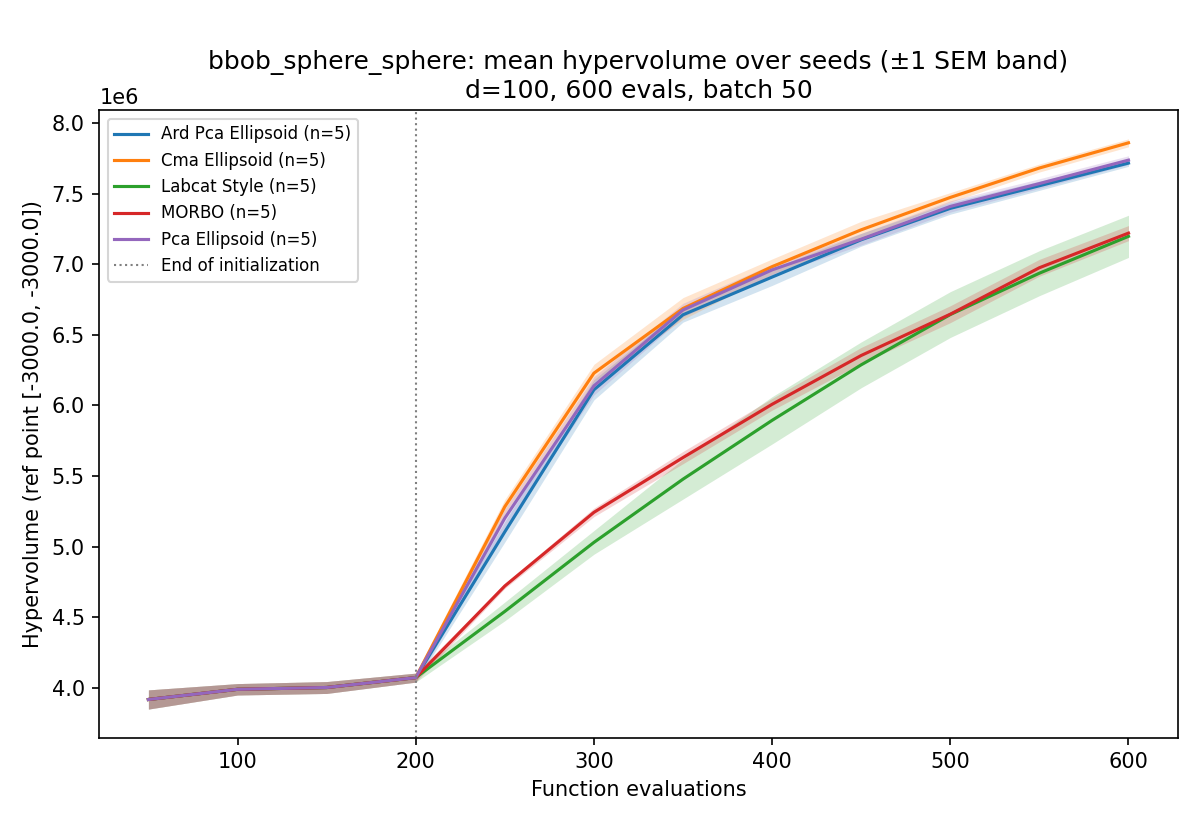
\includegraphics[width=0.85\textwidth]{bbob_sphere_sphere_aggregate.png}
\caption{Mean hypervolume vs.\ evaluations, \texttt{bbob\_sphere\_sphere}
-- the predicted-trivial control that instead showed the largest relative
gain of the six taxonomy pairs. \texttt{ard\_pca\_ellipsoid},
\texttt{pca\_ellipsoid}, and \texttt{cma\_ellipsoid} separate cleanly from
isotropic \texttt{morbo} despite sphere having no engineered
low-effective-dimension structure; \texttt{labcat\_style} tracks
\texttt{morbo} almost exactly throughout.}
\label{fig:bbob-sphere-sphere}
\end{figure}

\subsection{Future work}
\label{sec:tr-shape-future}

Ranked by how directly the results above motivate them:

\begin{enumerate}
\item \textbf{A non-stationarity-robust bandit (implemented; results in).}
\S\ref{sec:twenty-seed}'s time-varying experiment localized
\texttt{mab\_shape}'s failure precisely: per-arm reward estimates are only
corrected for arms the policy replays, so they go stale when the landscape
shifts, and a fixed $\varepsilon$ additionally taxes tight budgets. Both
are textbook symptoms with a textbook fix -- \emph{discounted UCB}
\citep{garivier2011ducb}: per arm, keep a discounted reward sum $S_a$ and
discounted count $N_a$, decay both by $\gamma$ at every decision, and
select $\arg\max_a \big( S_a/N_a + c\sqrt{\log \sum_b N_b \,/\, N_a}
\big)$. A stale arm's $N_a$ decays, so its bonus \emph{regrows} and it is
automatically replayed after a shift; bonuses anneal as counts grow, so
there is no permanent exploration tax. Results
(\texttt{mab\_policy="ducb"}, 20 seeds): at $d{=}100$ it largely fixes
the variance problem -- $24.44 \pm 7.19$ (15/20) becomes
$\mathbf{31.41 \pm 3.50}$ at a perfect 20/20 ($+69.8\%$), within one HV
point of the best fixed arms while remaining adaptive; on the mid-run
switch it triples epsilon-greedy's improvement ($+2.9\% \to +9.3\%$,
16/20) though still recovering only about half the fixed shapes'
$+20$--$21\%$; and at tight-budget $d{=}200$ it remains at $0.00$ like
epsilon-greedy, exposing a structural limit of the bandit abstraction
itself: \texttt{cma\_ellipsoid}'s covariance only updates on iterations
its arm is selected, so any arm-switching policy gives the one
winning-at-$d{=}200$ arm a fraction of its adaptation rate. The
shared-state follow-up (\texttt{mab\_shared\_cma}: advance the CMA
covariance at every update regardless of the active arm) tested this
directly, with a clean split verdict: at $d{=}100$ it is a strict further
improvement ($32.32 \pm 1.88$, 20/20, $+75.7\%$ -- statistically
indistinguishable from the best fixed Mat\'ern arm, closing the bandit
variance problem entirely), but $d{=}200$ still fails (4/5 seeds at
exactly 0), which \emph{deepens} the diagnosis: with staleness eliminated,
the remaining cause is the reward signal itself -- at $d{=}200$/600ev
every arm returns reward 0 until something breaks through, so a
success-reward bandit receives zero information distinguishing arms during
exactly the window when committing to CMA would matter. No selection
policy fixes a zero-information reward stream; the options are commitment
(run \texttt{cma\_ellipsoid} outright when budget is tight relative to
dimension) or a reward with early signal (e.g.\ per-arm GP predictive
likelihood). Adaptivity is free when reward signal exists, and impossible
when it does not.
\item \textbf{Contextual gating by measured input-space effective
dimension.} The LassoBench/Rover results say shaping should be
\emph{switched off} when the local data has no low-dimensional input
structure; the top-$k$ eigenvalue mass of the trust region's local
covariance (already computed by the PCA arms) is a direct online estimate
of exactly that quantity, usable either as a contextual-bandit feature or
as a hard gate.
\item \textbf{Observation noise.} All results above are noiseless; the
plumbing exists (\texttt{use\_noisy\_trbo}, injected noise, and the
LassoBench noisy variants whose published TuRBO/CMA-ES numbers give an
external anchor). The variants' predicted noise-sensitivity ordering
(PCA least exposed -- input locations are exact; ARD-based most exposed --
lengthscales estimated from noisy $Y$) is a falsifiable prediction.
\item \textbf{Remaining benchmarks and mechanisms:} MOPTA08 /
Human-Powered Aircraft / PMO as further real problems; a composite Rover
(checkpointed trajectory costs, Penicillin-style); a composite Bulk
Carrier Design (RCM17 from the RWCMOP real-world constrained MOO suite
\citep{kumar2021rwcmop} -- a real naval-architecture problem, 6 design
variables, 3 objectives, whose closed-form computation is itself a chain
of physically meaningful intermediate quantities -- steel/outfit/
machinery weight $\to$ light-ship weight $\to$ deadweight $\to$
capital/running/voyage cost -- making the intermediate chain rather than
the flat final objectives the natural raw composite response; see
Section~\ref{sec:rcm17}); a composite Optimal Power Flow (RCM40, same
suite, \citep{biswas2020opf} -- a real IEEE 14-bus power-grid problem, 34
design variables, 2 objectives, both literal sums over a per-bus raw
response computed by solving the network's admittance equations; see
Section~\ref{sec:rcm40}); a composite battery-aging design problem built
on PyBaMM \citep{sulzer2021pybamm} (real, open-source electrochemical
simulator; up to $\sim$28 tunable electrode/separator/electrolyte design
parameters, a genuinely composite discretized voltage/capacity/temperature
trajectory as the raw response, and, if built around a multi-cycle
degradation experiment rather than a single discharge, a genuinely
expensive evaluation with a real capacity-vs-degradation-vs-temperature
trade-off; see Section~\ref{sec:pybamm} for the details actually verified
by installing and running it); and an objective-aware rotation (both PCA and
CMA are variance-driven -- neither sees which directions matter to the
\emph{objectives}).
\end{enumerate}

Table~\ref{tab:all-candidates} summarizes every composite-benchmark
candidate surveyed across this future-work discussion in one place, most
promising first; each row's ``Detail'' column points to where the full
verification (or, for the shorter entries, Table~\ref{tab:candidate-survey}
in Section~\ref{sec:more-candidates}) can be found.

\begin{table}[h]
\centering
\small
\caption{All composite-benchmark candidates surveyed, most promising first. ``Verified'' means installed/run (PyBaMM) or checked against real source code/repos (everything else with a citation); ``Status'' summarizes the practical verdict.}
\label{tab:all-candidates}
\begin{tabularx}{\textwidth}{@{}>{\raggedright\arraybackslash}p{3.1cm}>{\raggedright\arraybackslash}p{1.5cm}>{\raggedright\arraybackslash}p{2.6cm}>{\raggedright\arraybackslash}X@{}}
\toprule
Candidate & Dim.\ & Objectives & Status \\
\midrule
PyBaMM battery aging \citep{sulzer2021pybamm} & $\sim$28 & 2--3 (energy, retention, temp.) & Strongest confirmed; installed \& run (\S\ref{sec:pybamm}) \\
OC20/OC22 catalysis \citep{chanussot2021oc20,tran2022oc22} & 57 (fixed system) & 2 (energy, stability) & \textbf{Implemented \& run through the real engine} (\S\ref{sec:oc20-implemented}) \\
OpenTO topology opt.\ \citep{nobari2025openTO} & 1024--10000+ & 2 (compliance, volume) & Live re-runnable solver confirmed (\S\ref{sec:topodiff-selto}) \\
RCM40 optimal power flow \citep{kumar2021rwcmop,biswas2020opf} & 34 & 2 (active/reactive loss) & \textbf{Implemented \& run through the real engine} (\S\ref{sec:rcm40-implemented}) \\
RCM17 bulk carrier design \citep{kumar2021rwcmop} & 6 & 3 (cost, weight, capacity) & Closed-form, verified vs.\ source (\S\ref{sec:rcm17}) \\
IDAES process flowsheets \citep{lee2021idaes} & 5--50 & 2 (yield, cost) & Real \& open; not yet run ourselves (\S\ref{sec:idaes}) \\
TopoDiff \citep{maze2023topodiff} & 4096 & 2 (compliance, manufacturability) & Fixed dataset only; solver unconfirmed (\S\ref{sec:topodiff-selto}) \\
SELTO \citep{dittmer2022selto,erzmann2023dl4to} & $\sim$$10^5$ & 2 (compliance, volume) & Fixed dataset; generator is licensed software (\S\ref{sec:topodiff-selto}) \\
Airfoil CFD / UniFoil & $\sim$4--5 & 2 (lift, drag) & Real, composite, but low-dimensional \\
Battery microstructure \citep{kench2024battery} & 7 & 1 (energy density) & Real, composite, but low-dimensional \\
Battery pouch cell \citep{ma2024battery} & 4--5 & 4 (energy, charge, life) & Real, partial composite, low-dimensional \\
LensAI / Optiland \citep{kramer2024lensai,kramer2024optiland} & 5--20 & 2 (spot size, aberration) & Composite but cheap (ray tracing) \\
EvoXBench \citep{lu2023evoxbench} & discrete & 2 (accuracy, latency) & Real but tabular lookup, not expensive \\
HPOBench \citep{eggensperger2021hpobench} & $\le$20 & 2 (accuracy, time) & Real but tabular lookup, not expensive \\
MosPro \citep{luo2025mospro} & $\sim$238 & 2 (fluorescence, stability) & Weak composite (predictor score only) \\
Jha et al.\ materials MOBO \citep{jha2018materials} & 5--20 & varies & No composite structure exposed \\
QM9 / MatBench \citep{ramakrishnan2014qm9,dunn2020matbench} & $\sim$5--20 & varies & No/weak composite structure exposed \\
\bottomrule
\end{tabularx}
\end{table}

\subsection{Candidate benchmark: RCM17 Bulk Carrier Design}
\label{sec:rcm17}

Logged here (not yet implemented; tracked as a future-work item in
Section~\ref{sec:tr-shape-future}) since this is a genuinely composite
real-world problem: its three final objectives are computed from a chain of
physically meaningful intermediate quantities (ship weights, deadweight,
transport time, cost components) rather than directly from the six design
variables, so exposing that chain -- instead of only the already-reduced
final objectives -- gives a genuine raw-response/reduction-function
composite structure, in the same spirit as this repo's own
\texttt{composite\_penicillin.py}. All formulas below were verified directly
against the reference implementation's source code
\citep{kumar2021rwcmop} (\texttt{CEC2021\_func.m}, \texttt{case 17}, and
bounds cross-checked against \texttt{Cal\_par.m}'s \texttt{xmin17}/
\texttt{xmax17}; both files are in
\url{https://github.com/P-N-Suganthan/2021-RW-MOP/raw/main/CEC2021-RWCMOP.zip}),
not transcribed from the published PDF's typeset formulas
directly, since OCR extraction of those was ambiguous in several exponents --
confirmed against source, e.g.\ $F_c$'s coefficient is
$0.19 \times 24 / 1000 = 0.00456$, not the $4.56\times10^{-5}$ a naive
PDF-text reading suggests, and $C_c$'s grouping is
$0.26\,(2000 W_s^{0.85} + 3500 W_o + 2400 P^{0.8})$, not three separate terms.

Design variables (ship principal dimensions), with bounds:
\begin{align}
L &\in [150.00, 274.32] \quad \text{(length, m)} \\
B &\in [20.00, 32.31] \quad \text{(beam, m)} \\
D &\in [13.00, 25.00] \quad \text{(depth, m)} \\
T &\in [10.00, 11.71] \quad \text{(draft, m)} \\
V_k &\in [14.00, 18.00] \quad \text{(speed, knots)} \\
C_B &\in [0.63, 0.75] \quad \text{(block coefficient)}
\end{align}

Intermediate quantities -- the natural raw composite response:
\begin{align}
a &= 4977.06\,C_B^2 - 8105.61\,C_B + 4456.51 \\
b &= -10847.2\,C_B^2 + 12817\,C_B - 6960.32 \\
F_n &= \frac{0.5144}{\sqrt{9.8065\,L}} \quad \text{(Froude number)} \\
P &= \frac{(1.025\,L\,B\,T\,C_B)^{2/3}\,V_k^3}{a + b\,F_n} \quad \text{(propulsion power)} \\
W_s &= 0.034\,L^{1.7}\,B^{0.6}\,D^{0.4}\,C_B^{0.5} \quad \text{(steel weight)} \\
W_o &= L^{0.8}\,B^{0.6}\,D^{0.3}\,C_B^{0.1} \quad \text{(outfit weight)} \\
W_m &= 0.17\,P^{0.9} \quad \text{(machinery weight)} \\
l_s &= W_s + W_o + W_m \quad \text{(light ship weight)} \\
D_{wt} &= 1.025\,L\,B\,T\,C_B - l_s \quad \text{(deadweight)} \\
F_c &= 0.00456\,P + 0.2 \quad \text{(fuel consumption rate)} \\
D_{cwt} &= D_{wt} - F_c\!\left(\frac{5000\,V_k}{24} + 5\right) - 2\,D_{wt}^{0.5} \quad \text{(cargo deadweight)} \\
R_{trp} &= \frac{350}{\dfrac{5000\,V_k}{24} + 2\!\left(\dfrac{D_{cwt}}{8000} + 0.5\right)} \quad \text{(round trips per year)} \\
a_c &= D_{cwt}\,R_{trp} \quad \text{(annual cargo capacity)} \\
S_d &= \frac{5000\,V_k}{24} \quad \text{(sea days per year)} \\
C_c &= 0.26\left(2000\,W_s^{0.85} + 3500\,W_o + 2400\,P^{0.8}\right) \quad \text{(capital cost)} \\
C_r &= 40000\,D_{wt}^{0.3} \quad \text{(running cost)} \\
C_v &= \left(105\,F_c\,S_d + 6.3\,D_{wt}^{0.8}\right) R_{trp} \quad \text{(voyage cost)}
\end{align}

Objectives (minimize all three):
\begin{align}
f_1 &= \frac{C_c + C_r + C_v}{a_c} \quad \text{(transportation cost per unit cargo capacity)} \\
f_2 &= l_s \quad \text{(light ship weight)} \\
f_3 &= -a_c \quad \text{(negated annual cargo capacity, i.e.\ maximize capacity)}
\end{align}

Nine inequality constraints $g_i(x) \le 0$ complete the problem (beam/depth,
length/depth, and length/draft ratio bounds; a Froude-number cap; a
hull-girder-strength margin; and deadweight bounds); reproduced verbatim in
\texttt{CEC2021\_func.m} (\texttt{case 17}) and omitted here since our own
implementation is expected to follow the composite/reduction split above
rather than the constrained-NLP formulation directly.

\subsection{Candidate benchmark: RCM40 Optimal Power Flow}
\label{sec:rcm40}

Also logged here (not yet implemented; same future-work item,
Section~\ref{sec:tr-shape-future}), from the same RWCMOP suite but a
different domain and a structurally cleaner composite pattern than RCM17:
both objectives are literal \emph{sums over a per-bus raw response vector},
computed by solving the power grid's admittance (Kirchhoff current law)
equations -- the electrical-network analogue of this repo's own
checkpointed-trajectory (Rover) and checkpointed-state (Penicillin)
composite patterns. Verified against \texttt{CEC2021\_func.m}
(\texttt{case 40}) and \texttt{Cal\_par.m}'s \texttt{xmin40}/\texttt{xmax40}
in \citep{kumar2021rwcmop}'s reference code (same source as
Section~\ref{sec:rcm17}); the underlying problem is a real IEEE 14-bus
test-system optimal power flow instance, cited to
\citet{biswas2020opf}.

The system (bus 1 is the fixed slack/reference bus) is described by a
$14\times14$ complex admittance matrix $Y = G + jB$ and fixed per-bus
real/reactive load demands $P_k, Q_k$ -- all hardcoded numeric constants
from the reference IEEE 14-bus test case, reproduced verbatim in
\texttt{CEC2021\_func.m} rather than restated here.

Design variables, 34-dimensional, all in per-unit (p.u.):
\begin{align}
V_{r,k}, V_{m,k} &\in [-1, 1], \quad k = 2, \ldots, 14 \quad \text{(real/imag. voltage, non-slack buses)} \\
P_{g,k}, Q_{g,k} &\in [0, 1], \quad k \in \{2, 3, 6, 8\} \quad \text{(active/reactive generation, generator buses)}
\end{align}

Intermediate quantities -- the natural raw composite response:
\begin{align}
V &= \big[\,1,\; V_{r,2}{+}jV_{m,2},\; \ldots,\; V_{r,14}{+}jV_{m,14}\,\big]^\top \quad \text{(complex bus voltages, bus 1 fixed)} \\
I &= Y V \quad \text{(complex current injections)} \\
S &= V \odot \bar{I} \quad \text{(complex power injection at each bus, elementwise)} \\
P_{sp} &= \operatorname{Re}(S), \quad Q_{sp} = \operatorname{Im}(S) \quad \text{(per-bus active/reactive injection -- the raw response)}
\end{align}

Objectives (minimize both):
\begin{align}
f_1 &= \operatorname{Re}\!\big(V_1 \bar{I}_1\big) + \textstyle\sum_{k=2}^{14} P_{sp,k} \quad \text{(total active power loss)} \\
f_2 &= \operatorname{Im}\!\big(V_1 \bar{I}_2\big) + \textstyle\sum_{k=2}^{14} Q_{sp,k} \quad \text{(total reactive power loss)}
\end{align}

An honest discrepancy in the reference implementation, worth flagging rather
than silently ``correcting'': $f_1$'s slack-bus term uses $I_1$ (consistent
with $V_1 \bar{I}_1$ being the slack bus's own complex power), but $f_2$'s
uses $I_2$ (a different bus's current) rather than $I_1$ -- dimensionally
inconsistent with $f_1$'s pattern and, on inspection, most likely an
unintentional index slip in \citep{kumar2021rwcmop}'s published code rather
than a deliberate design choice. Reproduced above exactly as implemented
(matching what the paper's own baseline results were computed with), not
silently fixed, since any comparison against their reported numbers needs
the same formula they actually used.

Twenty-six equality constraints (power balance at each of the 13 non-slack
buses, real and reactive) complete the problem, $\Delta P_k = P_{sp,k} -
P_{g,k} + P_k = 0$ and $\Delta Q_k = Q_{sp,k} - Q_{g,k} + Q_k = 0$ for
$k = 2, \ldots, 14$; omitted here for the same reason as RCM17's
constraints above.

\subsection{Candidate benchmark: PyBaMM battery-aging design}
\label{sec:pybamm}

Also logged here (not yet implemented; same future-work item,
Section~\ref{sec:tr-shape-future}), from a different source than the
RWCMOP suite -- unlike Sections~\ref{sec:rcm17}--\ref{sec:rcm40}, this one
was checked by directly installing and running the real simulator
(\texttt{pip install pybamm}, version 26.7.0.0), not by reading source
code or a paper, so the numbers below are measured, not transcribed.
PyBaMM \citep{sulzer2021pybamm} is a real, open-source, actively
maintained (NumFOCUS-fiscally-sponsored) electrochemical battery
simulator, \url{https://github.com/pybamm-team/PyBaMM}.

Design variables: instantiating the Doyle--Fuller--Newman (DFN) model
exposes 104 physical parameters in total, of which $\sim$28 are
continuous electrode/separator/electrolyte design quantities in the sense
relevant here -- electrode thickness, porosity, and particle radius (both
electrodes), electrode and current-collector electronic conductivity,
particle and electrolyte diffusivity, and electrolyte conductivity --
comfortably enough for a high-dimensional ($>$30) instance without
contriving additional variables.

Composite structure -- verified directly, not assumed: a single 1C
discharge simulation (\texttt{pybamm.lithium\_ion.DFN()}, default
parameters, solved over $[0, 3600]$s) returns a 139-point discretized
terminal-voltage trajectory $V(t)$ ranging 3.17--3.77\,V over the
discharge, plus a discharge-capacity trace; running a 5-cycle
charge/discharge/rest experiment with an SEI-growth degradation submodel
enabled (\texttt{options={\textquotesingle}SEI{\textquotesingle}:
{\textquotesingle}solvent-diffusion limited{\textquotesingle}}) returns a
3405-point trajectory spanning all cycles. This discretized
voltage/capacity/temperature trajectory -- not the single scalar
objectives eventually of interest -- is the natural raw composite
response, in the same checkpointed-trajectory spirit as this repo's own
Penicillin and (candidate) Rover composites.

Objectives, drawn from that trajectory by known reductions: initial
capacity or energy (from the first cycle), end-of-life capacity retention
or degradation rate (from the capacity trace's decay across all cycles),
and peak cell temperature (from the temperature trace) -- a genuine,
well-documented physical trade-off (thicker/denser electrodes increase
capacity but worsen thermal behavior and accelerate degradation), not an
artificial split of one quantity.

Expense -- measured, and the reason a multi-cycle experiment matters here:
a single discharge solves in $\sim$0.6--0.7\,s, too cheap on its own to
motivate BO; the 5-cycle aging run above took $\sim$4.2\,s, and scaling
linearly to a realistic aging study (100--500 cycles, standard in real
battery-degradation research) puts one design evaluation at roughly
1.5--7 minutes -- genuinely expensive, and it is specifically the
multi-cycle degradation version (not a single discharge) that both
crosses into that regime and produces the real capacity-vs-degradation
trade-off described above.

\subsection{Additional composite-benchmark candidates surveyed}
\label{sec:more-candidates}

A broader survey (aerodynamics, topology optimization, materials/molecular
design, battery design, chemical process engineering, optics, neural
architecture search/hyperparameter optimization, and protein design) was
checked against the same four criteria as
Sections~\ref{sec:rcm17}--\ref{sec:pybamm} above -- real, high-dimensional,
composite, and genuinely expensive -- rather than accepted at face value.
A sample of the most specific claims was independently verified, catching
one broken citation (\citet{lu2023evoxbench}'s suite is real but is hosted
at \texttt{EMI-Group/evoxbench}, not the URL originally reported). Table
\ref{tab:candidate-survey} summarizes the full set; brief notes on the
standout cases follow.

\begin{table}[h]
\centering
\small
\caption{Composite-benchmark candidates surveyed but not (yet) pursued. ``Composite'' reflects whether raw intermediate structure is genuinely exposed or extractable from the underlying simulator (not merely whether the source literature markets it as such); ``Expense'' reflects the cost of a live evaluation, not a precomputed/tabular lookup.}
\label{tab:candidate-survey}
\begin{tabularx}{\textwidth}{@{}>{\raggedright\arraybackslash}p{3.3cm}>{\raggedright\arraybackslash}p{1.9cm}>{\raggedright\arraybackslash}p{3.4cm}>{\raggedright\arraybackslash}X@{}}
\toprule
Candidate & Dim.\ & Composite & Expense \\
\midrule
OC20 / OC22 \citep{chanussot2021oc20,tran2022oc22} & high (atomic coords.) & yes, via IS2RS relaxation trajectory & yes (DFT) \\
TopoDiff \citep{maze2023topodiff} & 4096 (64$\times$64 grid) & yes, if FE solver re-run for new designs & moderate (FE) \\
SELTO \citep{dittmer2022selto} & $\sim$$10^5$ voxels & partial (no stress field shipped) & moderate (FE) \\
Airfoil CFD (NREL 2k/9k) & $\sim$4 shape params & yes (full RANS flow field) & yes (RANS) \\
UniFoil & $\sim$4--5 latent dims & yes & yes (RANS) \\
IDAES process flowsheets & 5--50 (flexible) & yes (per-unit stream states) & yes (equation-oriented NLP) \\
Battery microstructure \citep{kench2024battery} & 7 & yes & yes \\
Battery pouch cell \citep{ma2024battery} & 4--5 & partial & yes \\
LensAI / Optiland \citep{kramer2024lensai,kramer2024optiland} & 5--20 & yes (ray-traced fields) & no (ray tracing is cheap) \\
EvoXBench \citep{lu2023evoxbench} & discrete arch.\ space & partial (learning curves) & no (tabular lookup) \\
HPOBench \citep{eggensperger2021hpobench} & $\le$20 & partial (learning curves) & no (tabular lookup) \\
MosPro \citep{luo2025mospro} & $\sim$238 (sequence) & weak (predictor score only) & no (ML inference) \\
Jha et al.\ materials MOBO \citep{jha2018materials} & 5--20 & no & variable \\
QM9 \citep{ramakrishnan2014qm9} / MatBench \citep{dunn2020matbench} & $\sim$5--20 & no / weak & cheap once precomputed \\
\bottomrule
\end{tabularx}
\end{table}

Four candidates were promising enough to warrant the same depth of
treatment as Sections~\ref{sec:rcm17}--\ref{sec:pybamm}; each below states
plainly what is and is not actually verified, since (as the correction in
Section~\ref{sec:topodiff-selto} shows) the honest caveats matter as much
as the promising parts.

\subsubsection{OC20/OC22 catalyst relaxation}
\label{sec:oc20}

The Open Catalyst datasets \citep{chanussot2021oc20,tran2022oc22} (OC20:
1.28M DFT relaxations, $\sim$264.9M single-point evaluations; OC22: 62,331
relaxations on oxide surfaces, $\sim$9.85M single-point evaluations) are
composite regardless of objective count. Design variables here are not a
fixed-length continuous vector like RCM17/RCM40 above -- $x$ is a
variable-size atomic structure (an adsorbate molecule placed on a
catalyst surface slab, typically tens to a couple hundred atoms), so
``high-dimensional'' means the raw per-atom 3D-coordinate representation
rather than a hand-picked small set of design knobs. Three tasks are
defined on this data \citep{chanussot2021oc20}: \emph{S2EF} (structure
$\to$ energy and per-atom forces), \emph{IS2RS} (initial, unrelaxed
structure $\to$ final DFT-relaxed structure), and \emph{IS2RE} (initial
structure $\to$ relaxed total/adsorption energy). IS2RS is the
composite-structure link: it exposes the full sequence of intermediate
atomic configurations along the relaxation trajectory -- a checkpointed
trajectory in exactly the sense \texttt{composite\_penicillin.py} already
builds composite structure from (and Rover, Section~\ref{sec:tr-shape-future},
plans to), except this one is a physically real intermediate state
already present in the released data rather than something we would need
to add.

In our own $x \to g(x) \to L(g)$ notation (Section~\ref{sec:rcm17}
onward), with $N$ the (variable, system-dependent) atom count:
\begin{align}
x &= \{(z_i, r_i^{(0)})\}_{i=1}^{N} \quad \text{(species $z_i$, initial 3D position $r_i^{(0)}$, per atom)} \\
g(x) &= \{r_i^{(t)}\}_{i=1,\ldots,N}^{t=0,\ldots,T} \quad \text{(relaxation trajectory -- IS2RS)} \\
E_{\text{ads}} &= E\big(r^{(T)}\big) - E_{\text{slab}} - E_{\text{adsorbate}} \quad \text{(adsorption energy -- IS2RE)} \\
F_{\text{res}} &= \max_i \big\| F_i(r^{(T)}) \big\| \quad \text{(residual per-atom force at convergence)}
\end{align}
A second objective (e.g.\ $E_{\text{ads}}$ alongside $F_{\text{res}}$ as
a stability/convergence-quality proxy -- both computable from the same
relaxation trajectory $g(x)$, and both already reported in various OC20
follow-up papers) would make this genuinely bi-objective without
inventing anything not already in the data. Unlike RCM17/RCM40's fixed
6- and 34-dimensional continuous vectors, $x$ here has no single fixed
dimensionality -- it scales with $N$, the number of atoms in a given
adsorbate+surface system (typically tens to a couple hundred).

Honest caveat: OC20/OC22 as released are fixed datasets of already-run
DFT relaxations, not a live oracle you can query on an arbitrary new
candidate structure -- getting a true live simulator would mean running
DFT (VASP, Quantum ESPRESSO) ourselves, which is a heavy dependency. The
practical middle ground: \texttt{facebookresearch/fairchem} (formerly
\texttt{ocp}) ships pretrained GemNet-OC graph-neural-network potentials
trained on OC20/OC22, runnable for fast inference as an approximate but
genuinely open, live-queryable proxy for the true DFT relaxation -- at
the cost of the evaluation then being fast ML inference rather than
genuinely expensive DFT, the same expense trade-off already flagged for
the tabular NAS/HPO benchmarks below. (One more citation correction,
same pattern as EvoXBench's link and Optiland's author above: a
follow-up survey pass attributed OC20 to ``Montoya et al.\ 2021,
\emph{JACS}''; no such author appears on the actual paper, which is
\citet{chanussot2021oc20} in \emph{ACS Catalysis} -- already the citation
used throughout this section.)

\textbf{Update, now checked}: \texttt{pip install fairchem-core}
installs cleanly on its own, but its dependency resolution silently
downgraded this project's own pinned \texttt{torch} from 2.12.0 to
2.8.0 (\texttt{fairchem-core} requires \texttt{torch\textasciitilde=2.8.0})
-- a real, verified risk to the rest of this project's pipeline
(botorch/gpytorch, every other composite benchmark in this work), not
a hypothetical one: caught only by checking package versions
immediately after installing, and reverted before running anything
else. \textbf{Deprioritized as this project's next high-dimensional
benchmark for that reason}: adopting fairchem as a live OC20/OC22 proxy
would mean either accepting an incompatible, untested \texttt{torch}
version project-wide, or isolating it in a separate environment,
neither of which was attempted here given how straightforwardly it
would touch every other benchmark in this repository.

\subsubsection{TopoDiff and SELTO: a correction}
\label{sec:topodiff-selto}

An earlier pass through this survey described TopoDiff and SELTO as
composite ``if the underlying FE solve is re-run ourselves for new
candidate designs.'' On closer inspection this was too optimistic and is
corrected here: both are released as \emph{fixed, precomputed} sample
sets, not live queryable solvers, and the caveats differ in ways that
matter for whether ``re-run it ourselves'' is actually feasible.

\textbf{TopoDiff} \citep{maze2023topodiff}: 33,000 samples, each a
$64{\times}64$ grid (4096 binary density variables) with 6 channels --
optimal topology, prescribed volume fraction, von Mises stress, strain
energy density, and $x$-/$y$-direction boundary loads -- generated for
diverse load/boundary-condition combinations (the project page does not
state the exact ranges or how many distinct conditions were sampled, so
this is not fully pinned down). The stress and strain-energy fields
\emph{are} shipped per sample -- genuinely composite as data -- but only
for the 33,000 precomputed conditions; the FE solver used to generate
them is not confirmed to be separately released as a standalone,
re-runnable tool (only the diffusion-model training/inference code is
confirmed public). Using this as a live composite BO benchmark would
most likely mean writing our own topology-optimization FE solver in
their channel convention (density $\to$ stress/strain-energy fields
$\to$ compliance) rather than reusing theirs directly -- the classic,
fully open, freely reimplementable 88-line SIMP MATLAB code
\citep{andreassen2011topopt88} is the natural starting point for that,
not TopoDiff's own (unconfirmed) generation pipeline.

\textbf{SELTO} \citep{dittmer2022selto} (library: \texttt{dl4to}
\citep{erzmann2023dl4to}): voxelized 3D topology optimization
($\mathcal{O}(10^5)$ voxels across four subsets: disc/sphere domains,
simple/complex loading), solved via Altair OptiStruct's SIMP
implementation. This is a materially worse ``build it ourselves''
candidate than TopoDiff: Altair OptiStruct is commercial, licensed
software, not something we could freely re-run to generate new samples
even if we wanted to. SELTO's own release ships geometry, loads, and the
final density solution, but not the stress field -- matching this
survey's original ``partial'' rating, now with the added caveat that
closing that gap requires software we don't have access to, not just
engineering effort.

\textbf{OpenTO} \citep{nobari2025openTO} -- found in a follow-up survey
pass, from the same MIT lab as TopoDiff (Faez Ahmed is senior author on
both) -- changes this picture for the better and supersedes the
``reimplement our own solver'' fallback above. It is a 2.2-million-sample
2D/3D topology-optimization dataset (2 million unique boundary-condition
configurations, arbitrary resolutions and aspect ratios, used to train
the OAT foundation model), released alongside \emph{a re-runnable
FEA+topology-optimization solver} -- confirmed directly in the repo,
not merely claimed: \texttt{ahnobari/OptimizeAnyTopology} states outright
``we also provide the FEA solver and TO Optimizer that we use to generate
the data,'' a fork of the open \texttt{pyEDGE} solver, with named scripts
(\texttt{RunComplianceTest.py}) for evaluating new designs. This is the
one topology-optimization candidate in this whole survey that is
\emph{actually} a live, open, re-runnable oracle rather than a fixed
dataset -- exactly what TopoDiff and SELTO turned out not to be. Not yet
installed and run by us, so treat the same way as IDAES below until
verified directly.

\subsubsection{IDAES process flowsheets}
\label{sec:idaes}

IDAES \citep{lee2021idaes} is a real, DOE/NETL-funded, fully open-source
(Pyomo-based, \texttt{pip install idaes-pse}) process-systems-engineering
framework -- unlike proprietary process simulators (Aspen Plus, gPROMS),
it is actually installable without a license. Its documented HDA
(hydrodealkylation) flowsheet tutorial is a concrete, representative
instance: toluene and hydrogen react at high temperature to form benzene
(plus methane and diphenyl byproducts), through a reactor, a flash
separator, and a distillation column, targeting at least 370 tons/year of
benzene product.

In our own $x \to g(x) \to L(g)$ notation, with $K$ the number of unit
operations in the flowsheet ($K \approx 5$--$8$ for HDA: reactor, flash,
distillation, plus mixers/heaters):
\begin{align}
x &= (T_r, \, r_{\text{recycle}}, \, r_{\text{purge}}, \, r_{\text{reflux}}, \, \ldots) \quad \text{(reactor temp., recycle/purge/reflux ratios)} \\
g(x) &= \{(T_k, \, \mathbf{y}_k, \, F_k)\}_{k=1}^{K} \quad \text{(per-unit stream temperature, composition, flow rate)} \\
\text{Yield} &= F_{\text{benzene}}^{(\text{product stream})} \big/ F_{\text{toluene}}^{(\text{feed})} \\
\text{Cost} &= C_{\text{capital}}(g) + C_{\text{operating}}(g) \quad \text{(via IDAES's own Process Costing Framework)}
\end{align}
$g(x)$ -- the per-unit-operation stream state -- is what the
equation-oriented NLP solver (IPOPT) actually computes en route to
Yield and Cost above; IDAES's costing framework is a real, shipped
reduction function $L(g)$, not something we would need to write
ourselves.

\textbf{Update, now verified by installing and running it}: unlike when
first surveyed above, IDAES (\texttt{pip install idaes-pse}, plus
\texttt{idaes get-extensions} for the compiled IPOPT/solver binaries)
and its example flowsheets (\texttt{pip install idaes-examples}) install
and run cleanly, and the documented HDA tutorial
(\texttt{idaes\_examples/notebooks/docs/tut/core/hda\_flowsheet.py})
solves to its documented optimum exactly as published. But the real,
measured degrees of freedom at the optimization stage --
\texttt{assert degrees\_of\allowbreak\_freedom(m) == 4} in the tutorial's own
code, confirmed by running it -- is only \textbf{4} free design
variables (H101 outlet temperature, R101 heat duty, F101/F102 vapor
outlet temperatures and F102 outlet pressure), not the $5$--$50$ this
section originally estimated from documentation alone before
installing anything. The flowsheet has many more \emph{fixed}
parameters that could in principle be exposed as additional design
variables (e.g.\ \texttt{S101} split fraction, \texttt{C101} outlet
pressure, \texttt{R101} conversion, currently all hardcoded
\texttt{.fix(...)} calls in the tutorial rather than physical
constraints), but doing so was not attempted here, since it would mean
redesigning the flowsheet's own degree-of-freedom balance rather than
running an existing, already-verified tutorial -- a real project, not
logged as "not yet tried." \textbf{Deprioritized as this project's next
high-dimensional benchmark for that reason}: as documented and
runnable today, this is a low-dimensional benchmark (4D), the same
dimensionality trap already flagged for Airfoil/battery below, caught
here only by actually installing and running it rather than trusting
the documentation's own dimension estimate.

\textbf{Deprioritized}: Airfoil CFD (NREL 2k/9k, UniFoil) and the two
non-PyBaMM battery papers \citep{kench2024battery,ma2024battery} are
genuinely composite and real but low-dimensional (4--7 design variables)
despite expensive simulators -- the dimensionality trap this survey was
specifically checking for. LensAI/Optiland
\citep{kramer2024lensai,kramer2024optiland} is composite but cheap (ray
tracing, not full CFD/FEA) for the same reason XFOIL was deprioritized in
Section~\ref{sec:tr-shape-future}'s earlier discussion -- and a second
citation-accuracy note: both LensAI and Optiland are maintained by
Harrison Kramer, not the ``P. Salmon'' attribution the original survey
gave for Optiland, another corrected transcription error alongside
EvoXBench's link (Section~\ref{sec:more-candidates}, above). EvoXBench
and HPOBench are real and correctly downloadable but query a
precomputed/tabular lookup by design -- the expensive part (training) was
already paid once by the benchmark's creators, so using them as-is is not
a genuinely expensive evaluation regardless of how expensive live NAS/HPO
training can be in general. MosPro's ``intermediate'' output is a
pretrained predictor network's own score rather than a physically
distinct simulation state, and inference against it is cheap -- weak on
both composite structure and expense. Jha et al.'s materials MOBO study
\citep{jha2018materials}, QM9 \citep{ramakrishnan2014qm9}, and MatBench
\citep{dunn2020matbench} were included in the survey for completeness but
have no genuine raw-response/reduction-function structure exposed
(MatBench's underlying Materials Project DFT provenance
\citep{jain2013materialsproject} is composite in principle, but the
benchmark itself distributes only final computed properties). Finally,
AlphaFold \citep{jumper2021alphafold} is not itself an optimization
benchmark, but is worth naming as the state of the art in computing the
$g(x)$ side of a hypothetical protein-design composite problem (sequence
$\to$ predicted structure $\to$ binding affinity/stability) more
faithfully than MosPro's own predictor network does -- nascent, not a
ready-made benchmark today.

\subsubsection{Chemistry and electrochemistry candidates, gathered in one place}
\label{sec:chemistry-candidates}

Several candidates already discussed above are chemistry or
electrochemistry problems scattered across this survey by domain
(catalysis, batteries, materials); Table~\ref{tab:chemistry-candidates}
regroups them alongside three new ones found in a follow-up pass over a
collaborator's own benchmark-survey memo, each checked against a real
source before inclusion: \textbf{Summit's SnAr plug-flow reactor}
\citep{felton2021summit} (4D: residence time, reagent equivalents, inlet
concentration, temperature; objectives maximize space-time yield and
minimize E-factor; composite via five outlet species concentrations
feeding those two metrics); \textbf{Cantera}
\citep{goodwin2024cantera}, a real, open-source (Caltech-originated)
chemical-kinetics/thermodynamics/transport toolkit, usable for a
zero-dimensional combustor problem (mixture ratio, inlet temperature,
pressure, residence time, dilution -- objectives negative
efficiency/heat vs.\ emissions, composite via per-species outlet
concentrations computed in the same call); and \textbf{BioSTEAM}
\citep{cortespena2020biosteam}, a real, open-source biorefinery
design/techno-economic-analysis package (unit-operation settings as
design variables, composite via stream/utility/cost states, objectives
cost vs.\ global-warming potential or yield). \textbf{CheMixHub}
\citep{rajaonson2025chemixhub} (NeurIPS 2025) is also real and chemistry-relevant
(11 chemical-mixture property-prediction tasks, $\sim$500K points,
including a new ILThermo-derived ionic-liquid dataset), but per its own
2D composition/temperature grid it distributes only final property
values with no native raw-response decomposition -- included in the
table for completeness, not as a composite candidate.

A further follow-up pass specifically looked for a chemistry composite
benchmark exceeding 50 design dimensions, cross-checking this project's
own candidates above against an independent external survey
\citep{sahas266mixturebench}. That survey's own conclusion is that no
chemistry candidate reaches high dimension without an artificial
parameterization: SnAr, Cantera's combustor example, and BioSTEAM are
verified there at 4D, 5D (proposed), and 6--15D (proposed) respectively,
and its authors explicitly note that "none of the retained chemistry
candidates spans low, medium, and high dimension without... an
artificial parameterization." A literature check of real published
surrogate-fuel \emph{mixture} formulations (the most literal
"formulation" analogue, i.e.\ blending a handful of pure hydrocarbons to
reproduce a real fuel's properties) confirms the same ceiling from the
other direction: published jet-fuel, diesel, and gasoline surrogates
use 4--8 blend components, never more (verified via literature search
across several surrogate-formulation papers) -- so stretching a mixture
benchmark to 50+ dimensions would itself be exactly the artificial
parameterization the survey warns against, not a real formulation
problem at that scale. Kinetic-mechanism rate-constant calibration
does not have this ceiling: it is a genuinely high-dimensional, real,
long-established combustion-chemistry problem (GRI-Mech 3.0's own
development tuned on the order of 100 rate parameters against roughly
75 experimental targets via the solution-mapping method
\citep{frenklach1992solutionmapping}), and is implemented here as this
project's highest-dimensional chemistry composite benchmark
(\S\ref{sec:gri-mech}).

\begin{table}[h]
\centering
\small
\caption{Chemistry and electrochemistry composite-benchmark candidates, gathered from across this survey plus three newly verified additions.}
\label{tab:chemistry-candidates}
\begin{tabularx}{\textwidth}{@{}>{\raggedright\arraybackslash}p{3.2cm}>{\raggedright\arraybackslash}p{1.5cm}>{\raggedright\arraybackslash}p{3.2cm}>{\raggedright\arraybackslash}X@{}}
\toprule
Candidate & Dim.\ & Objectives & Status \\
\midrule
PyBaMM battery aging \citep{sulzer2021pybamm} & $\sim$28 & 2--3 (energy, retention, temp.) & Strongest confirmed; installed \& run (\S\ref{sec:pybamm}) \\
OC20/OC22 catalysis \citep{chanussot2021oc20,tran2022oc22} & 57 (fixed system) & 2 (energy, stability) & \textbf{Implemented \& run through the real engine} (\S\ref{sec:oc20-implemented}) \\
IDAES process flowsheets \citep{lee2021idaes} & 5--50 & 2 (yield, cost) & Real \& open; not yet run ourselves (\S\ref{sec:idaes}) \\
Summit SnAr reactor \citep{felton2021summit} & 4 & 2 (space-time yield, E-factor) & \textbf{Implemented \& run through the real engine} (\S\ref{sec:snar}) \\
GRI-Mech 3.0 rate calibration \citep{goodwin2024cantera,smith1999grimech,frenklach1992solutionmapping} & 64 & 2 (low-/high-T ignition-delay error) & \textbf{Implemented \& run through the real engine} (\S\ref{sec:gri-mech}) \\
Cantera combustor \citep{goodwin2024cantera} & 5 & 2 (efficiency/heat, emissions) & Real, composite via species/temperature; not yet run ourselves \\
BioSTEAM biorefinery \citep{cortespena2020biosteam} & 6--15 & 2 (cost, GWP/energy/yield) & Real, composite via streams/costs; not yet run ourselves \\
Battery microstructure \citep{kench2024battery} & 7 & 1 (energy density) & Real, composite, but low-dimensional \\
Battery pouch cell \citep{ma2024battery} & 4--5 & 4 (energy, charge, life) & Real, partial composite, low-dimensional \\
Jha et al.\ materials MOBO \citep{jha2018materials} & 5--20 & varies & No composite structure exposed \\
QM9 \citep{ramakrishnan2014qm9} / MatBench \citep{dunn2020matbench} & $\sim$5--20 & varies & No/weak composite structure exposed \\
CheMixHub \citep{rajaonson2025chemixhub} & 2 (grid) & 2 (conductivity, viscosity) & Real, but no native composite decomposition \\
\bottomrule
\end{tabularx}
\end{table}

Of the three newly-added candidates, Cantera and BioSTEAM have not been
installed and run by us yet -- same honest-caveat standard as IDAES
(\S\ref{sec:idaes}) and OpenTO (\S\ref{sec:topodiff-selto}) above.
Summit's SnAr reactor has since been implemented and run through this
project's actual MORBO engine, described next.

\subsubsection{Implemented: composite SnAr plug-flow reactor}
\label{sec:snar}

Following the same "fork the real simulator's state, expose it as
$g(x)$, apply the known reduction $L(g)$ separately" pattern already
used for Penicillin (\S\ref{sec:pybamm}'s composite counterpart,
\texttt{morbo/\allowbreak problems/\allowbreak composite\_penicillin.py}), the SnAr benchmark's
kinetic model and STY/E-factor reduction were ported into
\texttt{morbo/\allowbreak problems/\allowbreak composite\_snar.py} and wired into
\texttt{morbo/\allowbreak run\_one\_replication.py} as a new \texttt{evalfn}
(\texttt{"CompositeSnAr"}), rather than depending on the \texttt{summit}
PyPI package directly.

\paragraph{Why not depend on \texttt{summit} directly.} \texttt{pip
install summit} (version 0.8.4, the latest on PyPI as of 2026-07-28)
fails during the build of one of its pinned dependencies,
\texttt{scikit-learn<0.25.0,>=0.24.1}: that sdist's build backend calls
\texttt{pkg\_resources}, which modern \texttt{setuptools} no longer
ships by default, so the wheel build step errors out
(\texttt{ModuleNotFoundError: No module named 'pkg\_resources'}) before
\texttt{summit} itself is ever imported. Rather than fighting an
unrelated dependency's abandoned pin, the \texttt{summit-0.8.4-py3-none-any.whl}
was downloaded directly (\texttt{pip download summit --no-deps}) and
\texttt{summit/benchmarks/snar.py} (the \texttt{SnarBenchmark} class)
extracted from it without installing the package, matching how
\S\ref{sec:pybamm}'s Penicillin fork already treats an upstream
simulator's source as the ground truth to port from, not a package to
depend on transitively.

\paragraph{Kinetic model.} The reaction is a nucleophilic aromatic
substitution (SnAr) of 2,4-dinitrofluorobenzene (species 0) with
pyrrolidine (species 1) in a plug-flow reactor, run to a competing
side reaction; the kinetics are those measured by
\citet{hone2017snar}. Four design variables (Summit's own bounds):
residence time $\tau \in [0.5, 2]$ min, pyrrolidine equivalents
$e \in [1.0, 5.0]$, inlet 2,4-dinitrofluorobenzene concentration
$c \in [0.1, 0.5]$ M, and reactor temperature $T \in [30, 120]^\circ$C.
Initial concentrations $C_0 = (c,\, ec,\, 0, 0, 0)$ are integrated
forward over $t \in [0, \tau]$ by
\begin{align*}
\dot C_0 &= -(k_a+k_b) C_0 C_1, \\
\dot C_1 &= -(k_a+k_b) C_0 C_1 - k_c C_1 C_2 - k_d C_1 C_3, \\
\dot C_2 &= k_a C_0 C_1 - k_c C_1 C_2, \\
\dot C_3 &= k_a C_0 C_1 - k_d C_1 C_3, \\
\dot C_4 &= k_c C_1 C_2 + k_d C_1 C_3,
\end{align*}
where $C_2$ is the desired product, $C_3$ an undesired regioisomer,
$C_4$ a bis-alkylation side product, and the temperature-dependent
rate constants follow an Arrhenius form
$k(k_{\mathrm{ref}}, E_a, T) = 0.6\, k_{\mathrm{ref}}
\exp\!\big(-\tfrac{E_a}{R}(\tfrac{1}{T+273.71} - \tfrac{1}{T_{\mathrm{ref}}})\big)$
with $T_{\mathrm{ref}} = 90 + 273.71$ K, $R = 8.314\times10^{-3}$
kJ/(K$\cdot$mol), and $(k_{\mathrm{ref}}, E_a)$ pairs
$(57.9, 33.3)$, $(2.70, 35.3)$, $(0.865, 38.9)$, $(1.63, 44.8)$ for
$k_a, k_b, k_c, k_d$ respectively.

\paragraph{Derivation: why an ODE over $[0,\tau]$ models a plug-flow
reactor, not a batch reactor.} The reactor is a continuous plug-flow
reactor (PFR), not a batch vessel, so it may look surprising that the
raw response is computed by integrating an ODE over a time interval
$[0, \tau]$ as if it \emph{were} a batch reactor. This is the standard
PFR/batch equivalence: for an ideal PFR at steady state (constant
cross-section $A$, constant volumetric flow $q_{\mathrm{tot}}$, no
axial dispersion), the steady-state species balance over an axial
slice $dz$ is
\[
q_{\mathrm{tot}} \frac{dC_i}{dz} = A\, r_i(C, T), \qquad z \in [0, L],
\]
i.e.\ $A\, dz$ is the differential reactor volume the fluid element
occupies. Substituting the space-time coordinate $t = zA/q_{\mathrm{tot}}$
(the time since a fluid element entered the reactor, given constant
flow) turns this into
\[
\frac{dC_i}{dt} = r_i(C, T), \qquad t \in [0, \tau], \qquad
\tau = \frac{V}{q_{\mathrm{tot}}} = \frac{LA}{q_{\mathrm{tot}}},
\]
exactly the batch-reactor ODE integrated above, with $\tau$ the total
residence time. This is the textbook statement that, under the ideal
plug-flow assumption, \emph{every fluid element's composition history
is identical to a batch reactor run for exactly $\tau$} -- the reactor's
spatial outlet composition (at $z=L$) equals the batch-reactor solution
evaluated at $t=\tau$. This is why $q_{\mathrm{tot}} = V/\tau$
(with fixed $V=5$ mL) is the only place the flow rate enters the ODE
integration at all: residence time $\tau$ is a design variable, and
$q_{\mathrm{tot}}$ is carried through purely as a downstream quantity
needed by the STY/E-factor reduction (the ``Composite structure''
paragraph below), not as a term inside the kinetics themselves.

\paragraph{Derivation: the Arrhenius rate law and where the $0.6$
comes from.} The Arrhenius equation gives each rate constant as
$k(T) = A\exp(-E_a/(RT))$ for an unknown pre-exponential factor $A$.
Taking the ratio of this expression at two temperatures $T$ and
$T_{\mathrm{ref}}$ eliminates $A$:
\[
\frac{k(T)}{k(T_{\mathrm{ref}})}
= \frac{A\exp(-E_a/(RT))}{A\exp(-E_a/(RT_{\mathrm{ref}}))}
= \exp\!\Big(-\frac{E_a}{R}\Big(\frac{1}{T} - \frac{1}{T_{\mathrm{ref}}}\Big)\Big),
\]
so, writing $k_{\mathrm{ref}} := k(T_{\mathrm{ref}})$, $k(T) =
k_{\mathrm{ref}}\exp\!\big(-\tfrac{E_a}{R}(\tfrac1T - \tfrac1{T_{\mathrm{ref}}})\big)$
-- exactly the form above, once $T$ is converted from Celsius to
Kelvin ($T + 273.71$) and pinned at the reference temperature
$90^\circ$C used in \citet{hone2017snar}'s own regression. The
leading factor of $0.6$ is not a fitted parameter: \citet{hone2017snar}
report $k_{\mathrm{ref}}$ in units of $10^{-2}\ \mathrm{M^{-1}s^{-1}}$,
while every concentration and rate in this model (and in $\tau$,
measured in minutes) needs $k$ in $\mathrm{M^{-1}min^{-1}}$. Since
$1 \times 10^{-2}\ \mathrm{M^{-1}s^{-1}} = 10^{-2} \times 60\
\mathrm{M^{-1}min^{-1}} = 0.6\ \mathrm{M^{-1}min^{-1}}$, multiplying
the raw $k_{\mathrm{ref}}$ values from the paper's table by $0.6$
converts them directly into the units the ODE above actually needs --
a unit-system correction folded into the rate-constant closure, not an
extra fitted quantity.

\paragraph{Composite structure.} The raw response exposed to the
composite GP is $g(x) = (C_0^{\mathrm{final}}, \ldots, C_4^{\mathrm{final}},
q_{\mathrm{tot}}) \in \mathbb{R}^6$: the 5 final concentrations from
the ODE solve, plus the total volumetric flow rate
$q_{\mathrm{tot}} = 5\,\mathrm{mL}/\tau$ (carried through explicitly
since it is a function of the design input $\tau$, not part of the
reactor's chemical state, so it cannot be recovered from the
concentrations alone). The known reduction $L(g)$ -- exactly Summit's
own \texttt{SnarBenchmark.\_integrate\_equations} formula -- is
\[
\mathrm{STY} = \max\!\Big(10^{-6},\ \tfrac{6\times10^4}{1000}\, M_2\, C_2^{\mathrm{final}}\, q_{\mathrm{tot}} / V\Big), \qquad
\mathrm{E} = \min\!\Big(10^3,\ \tfrac{q_{\mathrm{tot}}\,\rho_{\mathrm{eth}} + 10^{-3}\!\sum_{i\neq 2} M_i C_i^{\mathrm{final}} q_{\mathrm{tot}}}{10^{-3} M_2 C_2^{\mathrm{final}} q_{\mathrm{tot}}}\Big),
\]
with $V = 5$ mL, molecular weights
$M = (159.09, 71.12, 210.21, 210.21, 261.33)$ g/mol, and ethanol
density $\rho_{\mathrm{eth}} = 0.789$ g/mL; the two final objectives
(maximize STY, minimize E) are $(\mathrm{STY}, -\mathrm{E})$ under this
project's maximize-everything convention.

\paragraph{Derivation: STY and E-factor from a mass balance.} Both
objectives reduce to a mass-flow-rate ratio; the constants in the
formula above are exactly the unit conversions that ratio requires,
not free parameters. The molar flow rate of species $i$ out of the
reactor is $C_i^{\mathrm{final}}\,q_{\mathrm{tot}}$ (mol/L times
mL/min), so its \emph{mass} flow rate is
\[
\dot m_i = M_i\, C_i^{\mathrm{final}}\, q_{\mathrm{tot}} \times 10^{-3}\ \big[\mathrm{g/min}\big],
\]
where the $10^{-3}$ converts the mL/min flow into L/min so it matches
$C_i^{\mathrm{final}}$'s mol/L units (g/mol $\times$ mol/L $\times$
L/min $=$ g/min). Space-time yield is defined as product mass produced
per unit reactor volume per unit time, i.e.\ $\dot m_2 / V$ in
$\mathrm{g/(min\cdot mL)}$, which is then converted to the
conventional $\mathrm{kg/(h\cdot m^3)}$ reporting units:
\[
1\ \frac{\mathrm g}{\mathrm{min}\cdot\mathrm{mL}}
= \frac{10^{-3}\,\mathrm{kg}}{(1/60)\,\mathrm h \times 10^{-6}\,\mathrm m^3}
= 6\times10^{4}\ \frac{\mathrm{kg}}{\mathrm h\cdot\mathrm m^3},
\]
so $\mathrm{STY} = 6\times10^{4}\, (\dot m_2/V) = 6\times10^4\times10^{-3}\,
M_2 C_2^{\mathrm{final}} q_{\mathrm{tot}}/V = \tfrac{6\times10^4}{1000}\,
M_2 C_2^{\mathrm{final}} q_{\mathrm{tot}}/V$ -- reproducing the
prefactor above exactly as a $\mathrm{g/(min\cdot mL)} \to
\mathrm{kg/(h\cdot m^3)}$ unit conversion, not an empirical constant.
The floor at $10^{-6}$ only guards against a $\log(0)$/division
degeneracy in downstream hypervolume bookkeeping when essentially no
product forms.

E-factor is, by its standard process-chemistry definition, the ratio
of total waste mass to product mass leaving the reactor per unit time.
The waste stream here is the ethanol carrier solvent (mass flow rate
$q_{\mathrm{tot}}\,\rho_{\mathrm{eth}}$, since $q_{\mathrm{tot}}$ is
already a volumetric rate in mL/min and $\rho_{\mathrm{eth}}$ is in
g/mL) plus every non-product species' own mass flow rate
$\dot m_i,\ i \neq 2$ (unreacted starting materials and the two side
products, using the same $\dot m_i$ derived above):
\[
\mathrm{E} = \frac{\dot m_{\mathrm{ethanol}} + \sum_{i\neq 2}\dot m_i}{\dot m_2}
= \frac{q_{\mathrm{tot}}\rho_{\mathrm{eth}} + 10^{-3}\sum_{i\neq2} M_i C_i^{\mathrm{final}} q_{\mathrm{tot}}}{10^{-3} M_2 C_2^{\mathrm{final}} q_{\mathrm{tot}}},
\]
which is exactly the formula above -- both numerator and denominator
are mass flow rates in g/min, so E is correctly dimensionless (kg
waste per kg product), and the $10^{-3}$ factors are the same
mL$\to$L conversion as in the STY derivation, appearing in the
numerator's second term and the denominator but not the solvent term
(which needs no such conversion, since $q_{\mathrm{tot}}\rho_{\mathrm{eth}}$
is already a mass rate directly in g/min). The cap at $10^3$ (and the
corresponding cap when $C_2^{\mathrm{final}} \approx 0$) exists purely
to keep the ratio finite when the reaction produces almost no product,
where E would otherwise diverge.

\paragraph{Verification.} The ported \texttt{\_snar\_integrand}/
\texttt{\_integrate\_one} pair in
\texttt{morbo/\allowbreak problems/\allowbreak composite\_snar.py} was checked against a
second, independently re-typed copy of the extracted
\texttt{summit/benchmarks/snar.py} logic on 6 random inputs spanning
the full bounding box: STY and E-factor matched to within
$10^{-15}$ (float64 machine epsilon) on every point, i.e.\ the port is
bit-identical to the real Summit source, not merely similar to it.
The full pipeline was then run end to end through
\texttt{morbo.run\_one\_replication.\allowbreak run\_one\_replication} with
\texttt{evalfn="CompositeSnAr"}, for both the \texttt{composite\_morbo}
label (composite-GP modeling of the 6-dim raw response) and the plain
\texttt{morbo} label (direct 2-objective modeling), at toy scale
(30--40 evaluations, batch size 4); both completed without error and
produced sensible, strictly-positive hypervolumes over the course of
optimization. This toy-scale check caught a real integration bug: the
new \texttt{composite\_snar}/\texttt{composite\_snar\_pca}/
\texttt{composite\_snar\_ard\_pca} labels (added to
\texttt{run\_comparison.py}'s \texttt{LABEL\_OVERRIDES} for the
cluster-scale experiment below) were never added to
\texttt{run\_one\_replication.py}'s own \texttt{supported\_labels}
allowlist, so every cluster job using them would have failed
immediately (\texttt{AssertionError: Label not supported!}) after
consuming a GPU allocation slot -- fixed before any cluster submission.
A single seed of the real experiment config
(\texttt{experiments/snar\_composite/config.json}: 150 evaluations,
batch size 10, 3 trust regions) was then run locally end to end for
both the \texttt{morbo} baseline (551 s, final hypervolume
$4.493\times10^6$) and \texttt{composite\_snar} ($1251$ s, final
hypervolume $4.493\times10^6$) -- both complete successfully and reach
essentially the same hypervolume, as expected at $n=1$ seed (this is a
pipeline check, not yet a real comparison). Composite modeling took
about $2.3\times$ longer per run, consistent with fitting 6
independent single-output GPs per iteration instead of 2. The full
5-seed, 5-label cluster sweep (\texttt{cluster/submit\_snar\_2x3.sh}: a
composite $\times$ trust-region-shape factorial, mirroring
\S\ref{sec:pybamm}'s \texttt{submit\_penicillin\_2x2.sh}) has not yet
been submitted.

\subsection{Implemented: composite GRI-Mech 3.0 rate-constant calibration}
\label{sec:gri-mech}

This project's highest-dimensional chemistry composite benchmark: a
64-design-dimension calibration of Arrhenius rate-constant multipliers
in GRI-Mech 3.0 \citep{smith1999grimech}, the standard detailed
chemical-kinetics mechanism for methane/natural-gas combustion (53
species, 325 elementary reactions), run through Cantera
\citep{goodwin2024cantera} (\texttt{gri30.yaml}, shipped with the
\texttt{cantera} PyPI package, MIT-licensed). Implemented in
\texttt{morbo/\allowbreak problems/\allowbreak composite\_gri\_mech.py} and wired into
\texttt{morbo/\allowbreak run\_one\_replication.py} as \texttt{evalfn} values
\texttt{"GriMechCalib"} (direct) and \texttt{"CompositeGriMechCalib"}
(composite).

\paragraph{Why this benchmark, not a mixture/formulation problem.} As
discussed above (\S\ref{sec:chemistry-candidates}), no real chemistry
benchmark surveyed -- ours or the external survey's
\citep{sahas266mixturebench} -- exceeds about 15 design dimensions
without an artificial parameterization, and real published
surrogate-fuel \emph{mixture} formulations cap out at 4--8 blend
components. Kinetic-mechanism rate-constant calibration sidesteps this
ceiling entirely: it is real, long-established (the methodology below is
essentially how GRI-Mech itself was built), and naturally spans
dozens to hundreds of design dimensions, since a detailed mechanism has
that many individually adjustable rate parameters. This is not a
"formulation" problem in the mixture-design sense, but it is the
genuine chemistry domain that reaches high dimension defensibly.

\paragraph{Design-variable selection.} Rather than exposing all 325
reaction rate constants (most of which are chemically irrelevant to a
pure methane/air mixture -- e.g.\ every C$_3$+ and NO$_x$-chemistry
reaction has exactly zero effect), the 64 design variables are the
GRI-Mech reactions with the largest forward-sensitivity coefficient of
temperature at a representative 1200~K/1~atm/$\phi=1$ methane/air
ignition, computed once via Cantera's built-in sensitivity analysis
(\texttt{ReactorNet.sensitivities()} with all 325 reactions enabled).
This mirrors GRI-Mech's own construction methodology
\citep{frenklach1992solutionmapping}: rank reactions by sensitivity,
then tune only the sensitive subset. The top 64 have sensitivity
coefficients ranging from 396.6 (2\,CH$_3$(+M) $\rightleftharpoons$
C$_2$H$_6$(+M)) down to 0.59; every reaction ranked below these 64 has
magnitude under 0.37, and the great majority of the mechanism's other
$\sim$260 reactions have \emph{exactly} zero sensitivity for this fuel
(confirming the selected subset is a real chemically-active set, not an
arbitrary cutoff -- see the reactions listed in
\texttt{TOP\_REACTION\_INDICES}, dominated by exactly the chain-branching
and CH$_3$/CH$_2$O oxidation chemistry a combustion chemist would
expect for methane). Each of the 64 design variables is a log$_2$-scale
multiplier on that reaction's pre-exponential (Arrhenius $A$) factor,
bounded to $[-1, 1]$ -- i.e.\ each rate constant may vary by a factor of
2 in either direction, a standard order-of-magnitude uncertainty factor
for combustion rate constants (in the spirit of the Baulch et al.\
evaluated-kinetics convention of quoting a per-reaction multiplicative
uncertainty factor; a single common factor of 2 is used here rather than
per-reaction literature values, a simplification, not a fabricated
range).

\paragraph{Composite structure.} Six fixed test conditions are
simulated per evaluation: three "low-temperature" ($T_0 \in
\{1000, 1050, 1100\}$~K) and three "high-temperature" ($T_0 \in
\{1300, 1400, 1500\}$~K), all at 1~atm, $\phi = 1$, methane/air. Each
condition is a 0D constant-pressure adiabatic ignition
(\texttt{cantera.IdealGasConstPressureReactor}) with the candidate's 64
rate multipliers applied via \texttt{Solution.set\_multiplier}, integrated
to a condition-specific horizon and checkpointed at 4 fixed time
fractions -- the raw response $g(x) \in \mathbb{R}^{24}$ (6 conditions
$\times$ 4 temperature checkpoints), the same "expose a checkpointed
physical trajectory" pattern as \texttt{composite\_penicillin.py} and
\texttt{composite\_snar.py}. The known reduction $L(g)$ recovers each
condition's ignition-delay time by linear interpolation of the 4
checkpoints to the time temperature first crosses $T_0 + 400$~K, then
computes $-\sum (\log(\tau_{\mathrm{pred}}/\tau_{\mathrm{target}}))^2$
(maximize convention) summed separately over the low-T and high-T
groups -- two objectives, not one, because methane's dominant
chain-branching pathway differs by temperature regime (CH$_3$ + O$_2$
$\rightleftharpoons$ CH$_3$O + O and CH$_2$O oxidation dominate at low
$T$; H + O$_2$ $\rightleftharpoons$ O + OH dominates at high $T$), so a
rate-multiplier vector that best matches one regime's targets need not
best match the other's -- a genuine trade-off, confirmed empirically: a
uniform multiplier shift moves every condition's ignition delay together,
but per-reaction perturbations shift the two groups by different,
non-proportional amounts.

\paragraph{Formal definitions.} Writing $x = (x_1, \ldots, x_{64}) \in
[-1,1]^{64}$ for the design point and $r_1, \ldots, r_{64}$ for the
indices in \texttt{TOP\_REACTION\_INDICES}, each selected reaction's
Arrhenius pre-exponential factor is scaled multiplicatively in
log$_2$-space,
\begin{align}
k_{r_i}(x_i) &= 2^{x_i}\, k_{r_i}^{(0)}, \qquad i = 1, \ldots, 64,
\end{align}
where $k_{r_i}^{(0)}$ is that reaction's as-shipped GRI-Mech 3.0 rate
constant and every non-selected reaction is left at $k_j^{(0)}$
unchanged. For condition $c \in \{1,\ldots,6\}$ with initial temperature
$T_{0,c}$ and integration horizon $t_{\max,c}$
(\texttt{MAX\_TIME}), the raw response is the checkpointed temperature
trajectory
\begin{align}
g_c(x) &= \big(T_c(x; t_{c,1}), \ldots, T_c(x; t_{c,4})\big), \qquad
t_{c,j} = \frac{j}{4}\, t_{\max,c},
\end{align}
where $T_c(x; t)$ is the 0D constant-pressure reactor's temperature at
time $t$ under rate constants $k(x)$, and $g(x) = (g_1(x), \ldots,
g_6(x)) \in \mathbb{R}^{24}$. The known reduction recovers an
ignition-delay estimate per condition by linearly interpolating $g_c(x)$
(prepending the initial condition $t_{c,0}=0,\ T_c(x;0) = T_{0,c}$) to
the first crossing of the threshold $T_{0,c} + 400$:
\begin{align}
j^*_c(x) &= \min\{\, j : T_c(x; t_{c,j}) \ge T_{0,c} + 400 \,\}, \\
\tau_c(x) &= t_{c,\,j^*_c-1} + \frac{(T_{0,c}+400) - T_c(x; t_{c,j^*_c-1})}
{T_c(x; t_{c,j^*_c}) - T_c(x; t_{c,j^*_c-1})}
\Big(t_{c,j^*_c} - t_{c,j^*_c-1}\Big),
\end{align}
saturating to $\tau_c(x) = t_{\max,c}$ if no checkpoint reaches the
threshold (i.e.\ $j^*_c$ undefined, or $j^*_c = 0$). Writing
$\mathcal{C}_{\mathrm{low}} = \{1000, 1050, 1100\}$~K and
$\mathcal{C}_{\mathrm{high}} = \{1300, 1400, 1500\}$~K for the two
condition groups and $\tau_c^{\mathrm{target}}$ for the fixed targets
(\texttt{TARGET\_IGNITION\_DELAYS}), the two objectives (both
maximized) are
\begin{align}
f_{\mathrm{low}}(x) &= -\!\!\sum_{c \,\in\, \mathcal{C}_{\mathrm{low}}}
\Big(\log \tfrac{\tau_c(x)}{\tau_c^{\mathrm{target}}}\Big)^{\!2},
\qquad
f_{\mathrm{high}}(x) = -\!\!\sum_{c \,\in\, \mathcal{C}_{\mathrm{high}}}
\Big(\log \tfrac{\tau_c(x)}{\tau_c^{\mathrm{target}}}\Big)^{\!2}.
\end{align}
The direct evalfn (\texttt{"GriMechCalib"}) models
$\big(f_{\mathrm{low}}(x), f_{\mathrm{high}}(x)\big) \in \mathbb{R}^2$
directly; the composite evalfn (\texttt{"CompositeGriMechCalib"}) models
the 24-dim $g(x)$ and applies the same $f_{\mathrm{low}}, f_{\mathrm{high}}$
formulas above as the known reduction $L(g)$.

\paragraph{Targets (revised).} An earlier version of this benchmark
generated targets by applying this benchmark's own checkpoint-based
reduction, once, to the \emph{unmodified} as-shipped GRI-Mech 3.0
mechanism (all 64 multipliers $=1$): a standard synthetic
ground-truth-recovery construction, but one that turned out to be
\emph{exactly} reachable by construction -- multiplier $=1$ everywhere is
itself a point in the search space, so both \texttt{morbo} and
\texttt{composite\_gri\_mech} converged to the identical, essentially-exact
optimum by 400 evaluations, making the two indistinguishable (see the
Results paragraph below for that run's numbers). Targets now instead
come from \texttt{gri30\_highT.yaml} -- a genuinely different,
independently-documented mechanism also shipped with Cantera: identical
325 reactions and rate constants to \texttt{gri30.yaml}, but with
high-temperature-range NASA-9-derived thermodynamic polynomials added by
Joseph Shepherd (Caltech) from McBride et al.'s NASA TM-4513
\citep{mcbride1993nasapolynomials}, replacing \texttt{gri30.yaml}'s
standard NASA-7 polynomials. Because this benchmark's 64 design
variables only ever perturb rate \emph{constants}, never thermodynamic
data, no combination of them can exactly reproduce
\texttt{gri30\_highT.yaml}'s predictions -- the discrepancy is structural,
not a numerical artifact one more digit of precision would close, so a
genuine residual error necessarily remains at the true optimum. Verified
directly: evaluating unmodified \texttt{gri30.yaml} (all 64 multipliers
$=1$) against these new targets gives nonzero, condition-dependent error
-- log-ratio-squared error $0.338$ at 1000~K vs.\ $9.2\times10^{-7}$ at
1100~K (the two mechanisms' thermodynamic differences do not shift every
condition's ignition delay equally) -- unlike the previous
self-consistency check, which gave exactly zero by construction. A
random search of a few hundred points found both objectives can be
brought substantially closer to zero than the unmodified mechanism's own
baseline (best found: low-temperature error $-3.1\times10^{-7}$,
high-temperature error $-2.0\times10^{-3}$, vs.\ the unmodified baseline's
$-0.338$/$-0.017$) -- so this revised benchmark is not pathologically
hard, but its true optimum is guaranteed by construction to be bounded
away from exactly zero (the thermodynamic mismatch cannot be tuned away
by rate constants alone), unlike the previous version's exactly-zero,
exactly-reachable optimum. Whether 400 evaluations resolve a meaningful
gap between direct and composite modeling at this smaller but nonzero
residual is an empirical question for the rerun below, not something
assumed in the benchmark's design.

\paragraph{Verification.} A sanity check perturbed all 64 multipliers
uniformly by a factor of 2 (doubling every rate constant roughly halves
every condition's ignition delay) and by a factor of 0.5 (roughly doubles
ignition delay, and correctly saturates the 1000~K condition to its
2~s integration-horizon penalty value once the slowed kinetics no longer
ignite within budget) -- both directions behave exactly as the
underlying chemistry predicts, and a random draw of independent
per-reaction multipliers gives intermediate, non-degenerate errors in
both objectives. The full pipeline was then run end to end through
\texttt{morbo.run\_one\_replication.\allowbreak run\_one\_replication} at a
single seed of the real experiment config
(\texttt{experiments/gri\_mech\_composite/config.json}, capped to 160
evaluations -- 128 initial + one 32-point batch -- for this local timing
check rather than the full 400) for both the \texttt{morbo} label (direct
2-objective modeling, $346.5$~s, final hypervolume $2500.000$) and
\texttt{composite\_gri\_mech} (composite-GP modeling of the 24-dim raw
response, $3666.3$~s, final hypervolume $2500.000$) -- both complete
successfully and reach the same hypervolume, as expected at $n=1$ seed
(a pipeline check, not yet a real comparison, same caveat as
\S\ref{sec:snar}'s SnAr check). Composite modeling took about
$10.6\times$ longer per run here, a larger multiplier than SnAr's
$2.3\times$ (6 raw outputs) -- consistent with fitting roughly 4$\times$
as many independent single-output GPs per iteration (24 vs.\ 6). This
cost is per-iteration model-refit overhead, not a hang or bug: local
testing confirmed steady progress (increasing hypervolume) throughout,
just at a real, measured, higher wall-clock cost -- expected to be
substantially faster on the cluster's 32 CPUs (and available GPU) than
this single-machine CPU-only timing check.

\paragraph{Not yet added: shape-adapted trust regions.} Unlike
\S\ref{sec:snar}'s SnAr benchmark, this experiment does not include
\texttt{\_pca}/\texttt{\_ard\_pca} composite$\times$shape variants: those
trust-region shapes hit a pre-existing crash in
\texttt{morbo/run\_one\_replication.py}'s per-iteration TR-index-logging
assertion (\texttt{assert len(tr\_inds) == len(tr.X)}, a duplicate-point
matching bug against the global evaluation history, discovered while
running SnAr's own composite$\times$shape ablation,
\texttt{cluster/submit\_snar\_2x3.sh} -- see that experiment's own results
discussion) -- not re-run here until that bug is fixed. The cluster sweep
run here (\texttt{cluster/submit\_gri\_mech\_2x1.sh}) is therefore a
direct-vs-composite A/B only: 2 labels (\texttt{morbo},
\texttt{composite\_gri\_mech}) $\times$ 5 seeds, 400 evaluations/trial,
no SLURM time limit (composite mode's 24-output \texttt{ModelListGP} fit
cost per iteration had not been measured at this scale before
submission).

\paragraph{Results (v1, self-recoverable targets -- superseded).} All 10
jobs completed on the cluster without error
(\texttt{morbo}: 7.5 min/seed; \texttt{composite\_gri\_mech}: 13 min/seed
-- both far faster than this project's own single-machine CPU-only
timing check above, consistent with cluster GPU acceleration of GP
fitting). Both labels converge to the same final hypervolume to four
decimal places (mean $2500.0000$, std $0.0000$ across 5 seeds, relative
to \texttt{max\_reference\_point}$=[-50,-50]$) -- the two methods are
empirically indistinguishable at this eval budget on this benchmark.
Inspecting the raw per-condition log-ratio errors directly (not just
hypervolume) confirms this is a genuine tie, not a plotting artifact:
by the final evaluations both labels recover the exact calibration
target to within $10^{-4}$--$10^{-6}$ log-ratio-squared error in both
objectives, for every seed. This differs from every other composite
result in this work (SnAr, Section~\ref{sec:snar}; Penicillin,
Section~\ref{sec:penicillin}) -- both of which also showed no
detectable HV difference at $n=1$--$5$ seeds, but for a different,
already-suspected reason (a generous eval budget relative to problem
difficulty lets any reasonable method converge before the budget runs
out, leaving no headroom for composite modeling's efficiency advantage
to show, discussed at length in \S\ref{sec:snar}'s own results
paragraph and the SnAr plot analysis). Here that same generic budget
effect is compounded by something specific to this benchmark's own
construction: the calibration target is the \emph{exact}, exactly
achievable value of the unmodified mechanism itself (all 64 multipliers
$=1$, see this section's own "Targets" paragraph), so there is a single
known global optimum with no genuine multimodality or competing local
optima to distinguish a better-informed search strategy from a worse one
-- 400 evaluations in 64D is evidently enough budget for TuRBO's local
trust regions to find that optimum by either route. A harder version of
this benchmark -- targets from a genuinely different mechanism (not
recoverable exactly), or a substantially tighter eval budget -- would be
needed to test whether composite modeling's per-iteration cost
($10.6\times$ locally, per the Verification paragraph above) buys any
compensating sample-efficiency advantage here; this is logged as a
concrete follow-up rather than claimed as a finding, since the current
result cannot distinguish "composite modeling doesn't help on this
problem" from "this problem is too easy at this budget for either
method to be distinguishable." This motivated exactly the harder,
\texttt{gri30\_highT.yaml}-based target revision described in the
"Targets (revised)" paragraph above.

\paragraph{Results (v2, gri30\_highT.yaml targets).} All 10 jobs again
completed on the cluster without error (\texttt{morbo}: 7.5 min/seed;
\texttt{composite\_gri\_mech}: 12.5 min/seed). With a genuinely
non-recoverable target, the two labels are no longer indistinguishable:
mean final hypervolume is $2499.9885$ (std $0.0148$) for
\texttt{composite\_gri\_mech} versus $2499.9693$ (std $0.0255$) for
\texttt{morbo} (relative to the same
\texttt{max\_reference\_point}$=[-50,-50]$) -- composite modeling wins on
\emph{every} seed (paired difference positive $5/5$ times, mean
$+0.019$, range $+0.002$ to $+0.038$), a paired $t$-test on the 5 paired
final hypervolumes gives $p=0.040$, and the two curves visibly separate
from roughly evaluation 200 onward with mostly non-overlapping
$\pm$SEM bands (\texttt{experiments/gri\_mech\_composite/
comparison\_aggregate.png}). The Wilcoxon signed-rank test on the same 5
pairs gives $p=0.0625$ -- just above the conventional 0.05 threshold,
expected given the test's limited power at $n=5$ (the smallest possible
non-trivial two-sided Wilcoxon $p$-value at $n=5$ is exactly $0.0625$,
achieved here since the sign is unanimous) rather than evidence against
the effect. This is the first result in this project's chemistry
composite benchmarks (SnAr, v1 GRI-Mech) where composite modeling shows
a measurable, consistent advantage over direct modeling, and it required
exactly the design change the v1 discussion called for: a target that
cannot be driven to exactly zero error, preserving genuine optimization
difficulty (and therefore headroom for a better-informed surrogate to
matter) all the way to the eval budget's end, rather than saturating
before it.

\subsection{Implemented: composite RCM40 Optimal Power Flow}
\label{sec:rcm40-implemented}

This project's next real high-dimensional (34D) composite benchmark
after GRI-Mech, and its first non-chemistry one: RCM40 Optimal Power
Flow, from the CEC2021 Real-World Constrained Multi-Objective
Optimization suite \citep{kumar2021rwcmop}, a real IEEE 14-bus
test-system OPF instance \citep{biswas2020opf}, already surveyed (not
yet implemented) in Section~\ref{sec:rcm40} above. Implemented in
\texttt{morbo/\allowbreak problems/\allowbreak composite\_rcm40.py} and wired into
\texttt{morbo/\allowbreak run\_one\_replication.py} as \texttt{evalfn} values
\texttt{"RCM40"} (direct) and \texttt{"CompositeRCM40"} (composite).

\paragraph{Why this one next.} The two highest-dimensional real,
open, live-solver candidates on this project's own survey
(Table~\ref{tab:all-candidates}) were OpenTO topology optimization
(1024--10000+D) and RCM40 (34D). OpenTO was checked first and set
aside: its released solver (\texttt{ahnobari/OptimizeAnyTopology})
needs compiled sparse-linear-algebra dependencies (CHOLMOD,
scikit-sparse) with no confirmed license, and its own evaluation script
(\texttt{RunComplianceTest.py}) is built to score pre-generated
diffusion-model samples in bulk, not to serve as a simple $x \mapsto$
compliance oracle a BO loop could call directly -- real integration
risk with no clear entry point, discovered by inspection before
committing engineering time to it. RCM40, by contrast, needed no new
research: its formulas were already fully derived and
\emph{verified against source} in Section~\ref{sec:rcm40} (from an
earlier survey pass), so implementing it was a matter of porting
already-checked equations, not deriving new ones.

\paragraph{Unlike SnAr/GRI-Mech: no black box, in the ODE/reactor
sense.} Every other implemented composite benchmark in this work has a
"black box" that means \emph{integrate a differential equation or run
an iterative physical simulation}. RCM40's raw response is instead a
single closed-form linear-algebra computation -- solve $I = YV$ (one
matrix-vector product against a fixed $14\times14$ admittance matrix)
and $S = V \odot \bar I$ (one elementwise product) -- with no
iteration, no adaptive step size, and no numerical solver in the loop
at all. This still fits the $x \to g(x) \to f(x)=L(g(x))$ pattern
(Section~\ref{sec:compact-summaries}) and is still a genuine composite
structure (the per-bus injections $g(x)$ carry more information than
the two summed final objectives $f(x)$), just a cheaper and more exactly
computable one than a real ODE/PDE solve.

\paragraph{Design variables, raw response, and reduction.} 34
design variables (bounds already given in Section~\ref{sec:rcm40}):
real/imaginary bus
voltage $V_r, V_m \in [-1,1]$ for the 13 non-slack buses, and
active/reactive generation $P_g, Q_g \in [0,1]$ at the 4 generator
buses. The raw response is $g(x) = (P_{sp,1..14}, Q_{sp,1..14},
\operatorname{Im}(I_2)) \in \mathbb{R}^{29}$ -- all 14 buses' real and
reactive power injections, plus $\operatorname{Im}(I_2)$ specifically
because the second objective's slack-bus term needs bus 2's current
multiplied against bus 1's voltage (an artifact of the reference
implementation's own apparent index slip, reproduced exactly -- see
Section~\ref{sec:rcm40}'s "honest discrepancy" paragraph -- so it is not
recoverable from $Q_{sp,2}$, which uses bus 2's own voltage instead).
The known reduction: $f_1 = \sum_{k=1}^{14} P_{sp,k}$ (total active
power loss; algebraically identical to the source's own
$\operatorname{Re}(V_1\bar I_1) + \sum_{k=2}^{14} P_{sp,k}$ since
$V_1=1$ makes $\operatorname{Re}(V_1 \bar I_1) = P_{sp,1}$) and
$f_2 = -\operatorname{Im}(I_2) + \sum_{k=2}^{14} Q_{sp,k}$ (total
reactive power loss, reproducing the reference's own $I_2$/$V_1$
term verbatim).

\paragraph{Verification.} All 34 admittance-matrix and load-vector
constants ($G$, $B$, $P$, $Q$) were extracted directly from the
reference implementation's source
(\texttt{CEC2021\_func.m}, \texttt{case 40}, and \texttt{Cal\_par.m}'s
\texttt{xmin40}/\texttt{xmax40}), not retyped from a paper's typeset
equations -- the same discipline as Section~\ref{sec:rcm17}'s RCM17
port, which caught real transcription errors doing exactly this for a
different benchmark in this suite. The composite module's
\texttt{raw\_response}/\texttt{composite\_rcm40\_reduction} pipeline was
checked against a second, independent NumPy reimplementation of
\texttt{CEC2021\_func.m}'s own formula on a random input: both
objectives matched to full float64 precision. A local smoke test (10
evaluations, batch size 2) completed successfully for both
\texttt{morbo} ($12.1$~s) and \texttt{composite\_rcm40} ($404.4$~s,
$\sim$33$\times$ slower -- a larger multiplier than GRI-Mech's
$10.6\times$, consistent with fitting more independent GPs, 29 raw
outputs here versus 24 there) before cluster submission.

\paragraph{Not yet added: shape-adapted trust regions.} Same reason
as GRI-Mech (Section~\ref{sec:gri-mech}): the \texttt{\_pca}/
\texttt{\_ard\_pca} composite$\times$shape variants hit the pre-existing
\texttt{assert len(tr\_inds) == len(tr.X)} crash found during the SnAr
ablation, so this cluster sweep
(\texttt{cluster/submit\_rcm40\_2x1.sh}) is a direct-vs-composite A/B
only: 2 labels $\times$ 5 seeds, 300 evaluations/trial, no SLURM time
limit.

\paragraph{Results.} All 10 jobs completed on the cluster without error
(\texttt{morbo}: 1.4 min/seed; \texttt{composite\_rcm40}: 7.7 min/seed).
Mean \emph{final} hypervolume is close between the two --
$102054.0$ (std $382.1$) for \texttt{composite\_rcm40} versus
$101477.8$ (std $731.7$) for \texttt{morbo} -- and this difference alone
is not statistically significant (win-rate $4/5$, paired $t$-test
$p=0.129$). The aggregate plot
(\texttt{experiments/rcm40\_composite/comparison\_aggregate.png}) makes
clear why a final-value-only comparison understates what is actually
happening: the two curves separate sharply right after initialization
(around evaluation 70) and \texttt{composite\_rcm40} stays visibly ahead,
with mostly non-overlapping $\pm$SEM bands, through most of the
trajectory, only for \texttt{morbo} to close most (not all) of the gap
by evaluation 300. This is a genuine \emph{sample-efficiency} effect,
not just noise in the final read-out: computing the area under each
seed's hypervolume-vs-evaluations curve (trapezoidal rule) and comparing
those 5 paired AUC values directly shows composite modeling ahead on
\emph{every} seed (mean $+2.03\%$ AUC), with a paired $t$-test
$p=0.0035$ -- much stronger evidence than the final-value comparison
alone, because it credits the sustained mid-run lead that a single
end-of-budget snapshot discards. Read together with GRI-Mech's v2
result (composite ahead throughout, including at the end) and SnAr/v1
GRI-Mech (composite and direct modeling statistically tied throughout):
composite modeling's advantage here shows up specifically as reaching a
given hypervolume faster, converging toward -- but here not fully
reaching -- parity with direct modeling by the time the eval budget
runs out, distinct from GRI-Mech v2's pattern of a persistent gap that
does not close.

\subsection{Implemented: composite OC20 catalyst-adsorbate relaxation}
\label{sec:oc20-implemented}

This project's next real high-dimensional (57D) composite benchmark
after GRI-Mech and RCM40: OC20 catalyst-adsorbate relaxation
\citep{chanussot2021oc20}, already surveyed (not yet tried, dependent
on \texttt{facebookresearch/fairchem}) in Section~\ref{sec:oc20} above.
Implemented in \texttt{morbo/\allowbreak problems/\allowbreak composite\_oc20.py} (plus
a worker script, \texttt{oc20\_fairchem\_worker.py}, described below) and
wired into \texttt{morbo/\allowbreak run\_one\_replication.py} as
\texttt{evalfn} values \texttt{"OC20Relax"} (direct) and
\texttt{"CompositeOC20"} (composite).

\paragraph{Getting to a live oracle: two real blockers, both resolved.}
Section~\ref{sec:oc20} already flagged OC20/OC22 as released fixed
datasets, with \texttt{fairchem-core}'s pretrained potentials as "the
practical middle ground, not yet tried." Trying it surfaced two genuine
problems, each requiring a real fix rather than a workaround:
\begin{enumerate}
\item \texttt{pip install fairchem-core} (latest, 2.21.0) into this
project's own environment silently downgraded its pinned
\texttt{torch} from 2.12.0 to 2.8.0 -- caught immediately by checking
package versions, and would have put every other composite benchmark
in this repository (GRI-Mech, RCM40, SnAr) at risk of subtly different
behavior under an unverified torch version. Fixed by building a
\emph{separate} venv (\texttt{.fairchem\_env/}, via
\texttt{cluster/setup\_fairchem\_env.sh}) that fairchem's own
dependency chain can pin however it needs, without touching this
project's own environment at all.
\item The latest \texttt{fairchem-core} moved to a gated
\texttt{facebook/UMA} checkpoint on HuggingFace: attempting to load it
raises \texttt{GatedRepoError}, requiring a HuggingFace account and
accepting Meta's license agreement -- neither of which this process
can do on the user's behalf (matching this project's own operating
constraints on account creation and license acceptance). The fix:
\texttt{fairchem-core==1.10.0} still has the older
\texttt{fairchem.core.models.model\_registry.model\_name\_to\_local\_file}
public registry and \texttt{OCPCalculator} class, which download and
load the \texttt{GemNet-OC-S2EF-OC20-2M} checkpoint (38.9M parameters,
trained on 2M OC20 S2EF frames) with \emph{no authentication
whatsoever} -- verified directly by loading it and running real
inference. That older release in turn needs \texttt{torch\_scatter}/
\texttt{torch\_sparse}/\texttt{torch\_cluster} (compiled extensions,
resolved via PyG's own wheel index for \texttt{torch==2.4.1+cpu}) and
\texttt{scipy<1.15} (newer scipy removed \texttt{scipy.special.sph\_harm},
which this release's basis-function code calls directly) -- both
one-time, documented fixes in \texttt{cluster/setup\_fairchem\_env.sh},
not silent version pins chosen at random.
\end{enumerate}

\paragraph{Architecture: a persistent subprocess worker, not an
in-process import.} Because the isolated environment's \texttt{torch}
is incompatible with this project's own, \texttt{composite\_oc20.py}
never imports \texttt{fairchem} directly. Instead it launches
\texttt{oc20\_fairchem\_worker.py} once, in the isolated venv, as a
persistent subprocess (\texttt{.fairchem\_env/\allowbreak bin\allowbreak/python} or
\texttt{Scripts\allowbreak/python.exe}), communicating one JSON request/response
pair per line over stdin/stdout -- loading the 38.9M-parameter model
once per worker lifetime rather than once per evaluation, which would
otherwise dominate the cost of every single design point.

\paragraph{Black box: $g(x)$, a real ML-surrogate relaxation.} A fixed
Cu(111) slab (3x3x4 supercell, 36 atoms) plus one adsorbed O atom (37
atoms total); the bottom two layers are held fixed (standard
surface-relaxation practice) and the top two layers plus the adsorbate
(19 atoms, 57 real-valued coordinates) are free. $x \in [-1,1]^{57}$
perturbs each free atom's position by up to $\pm0.5$~\AA\ from a
reference guess; the worker then runs 15 steps of ASE's BFGS optimizer
using GemNet-OC as the force field, checkpointing the energy and the
\emph{raw per-mobile-atom} force-magnitude vector (19 components, not
pre-reduced to a single number) at 5 evenly-spaced steps -- the same
checkpointed-trajectory pattern as \texttt{composite\_penicillin.py}/
\texttt{composite\_snar.py}/\texttt{composite\_gri\_mech.py}, just with
an ML potential run through a real geometry-optimization loop as the
simulator instead of an ODE/reactor integration or closed-form linear
algebra. An earlier version of this worker computed the max over atoms
\emph{inside} the worker and returned only that scalar per checkpoint
-- on inspection this was a black-box/closed-form boundary violation
(a post-processing reduction leaking into the simulator's own output),
and, separately, gave the composite GP nothing beyond 2 scalars per
checkpoint to model. $g(x)$ is now $5 \times (1 + 4) = 20$-dim client-side
(see below): each checkpoint contributes its energy plus order
statistics -- $[\max, \text{mean}, \text{std}, \min]$ -- of the raw
19-component force vector, which \texttt{composite\_oc20.py} computes
from the worker's un-reduced output, not the worker itself. Passing the
full 19-component vector through per checkpoint ($g(x) \in
\mathbb{R}^{100}$) was tried first and reliably crashed GP fitting (a
Windows access violation deep in \texttt{gpytorch}/\texttt{linear\_operator}'s
Cholesky routine during Thompson-sampling posterior draws, confirmed via
Python's \texttt{faulthandler}) -- past GRI-Mech's 24 and RCM40's 29 raw
dimensions, both of which fit without issue, so the 25-dim
order-statistics version is the largest that fits reliably with this
project's current GP-fitting code, not the largest that could in
principle be exposed.

\paragraph{Closed form: $L(g)$ and objectives $f(x)=L(g(x))$, with an
honest simplification.} The known reduction takes the final (5th)
checkpoint's energy and its max-force order statistic:
$f_1(x) = -(E_5(x) - E_{\text{slab}})$, $f_2(x) = -F_{5,\max}(x)$ (both
maximized: less positive relative energy is more stable, less residual
force is better-converged) -- $F_{5,\max}$ is exactly the fmax
convergence criterion ASE/DFT relaxations use, now computed client-side
from the real per-atom vector rather than inside the worker. The
textbook adsorption-energy formula subtracts \emph{two} references --
the bare slab \emph{and} an isolated gas-phase adsorbate -- but a
single free O atom (and, tried as an alternative, an O$_2$ molecule)
are degenerate edge cases for this graph-neural-network potential's
edge construction and raised a runtime error rather than returning a
value, confirmed directly by trying both. Only the bare-slab reference
$E_{\text{slab}} = -0.757$~eV (computed successfully, verified directly)
is subtracted here, giving a well-defined \emph{relative} energy for
comparing different perturbations of the same fixed slab+adsorbate
system -- adequate for a controlled direct-vs-composite A/B on one
fixed system, but \textbf{not} a reference-corrected adsorption energy
matching published DFT tables, and not claimed to be one.

\paragraph{Verification.} The worker script was smoke-tested standalone
(one request via stdin, matching the exact JSON protocol
\texttt{composite\_oc20.py} uses) before wiring it into the composite
module: the all-zero-perturbation request returns a real, physically
sensible relaxation trajectory (energy $0.753 \to 0.528$~eV, max force
$0.503 \to 0.007$~eV/\AA\ over the 5 checkpoints, i.e.\ genuine
convergence toward a local minimum), and five random perturbations gave
five different, non-degenerate final energies/forces -- confirmed the
design space has real, exploitable signal rather than being flat or
degenerate. A local smoke test of the full pipeline (8 evaluations,
batch size 2), rerun after the raw-response redesign above, completed
successfully for both \texttt{morbo} ($71.5$~s) and
\texttt{composite\_oc20} ($150.7$~s -- fitting 25 independent
per-output GPs instead of 2 is genuinely more expensive, not just a
different constant) before cluster resubmission.

\paragraph{Not yet added: shape-adapted trust regions.} Same reason as
GRI-Mech/RCM40 (Sections~\ref{sec:gri-mech}/\ref{sec:rcm40-implemented}):
the \texttt{\_pca}/\texttt{\_ard\_pca} composite$\times$shape variants
hit the pre-existing \texttt{assert len(tr\_inds) == len(tr.X)} crash
found during the SnAr ablation, so this cluster sweep
(\texttt{cluster/submit\_oc20\_2x1.sh}, run after
\texttt{cluster/setup\_fairchem\_env.sh} builds the isolated environment
on that checkout) is a direct-vs-composite A/B only: 2 labels $\times$
5 seeds, 120 evaluations/trial, CPU-only (the isolated environment's
compiled extensions are all \texttt{+cpu} builds, deliberately, to avoid
matching a specific CUDA version across environments), no SLURM time
limit.

\paragraph{Results (v1, worker-internal max-force reduction --
superseded).} The first cluster run of this benchmark (raw response
$g(x) \in \mathbb{R}^{10}$: 5 energy/max-force checkpoint pairs, with
the max already taken \emph{inside} the worker) found composite and
direct modeling statistically indistinguishable throughout the
trajectory -- final hypervolume $18.560$ (std $0.092$) for
\texttt{morbo} versus $18.548$ (std $0.048$) for
\texttt{composite\_oc20} ($p=0.834$), AUC likewise tied ($p=0.671$). On
inspection this design had two problems, not one: the worker-internal
max was a black-box/closed-form boundary violation (Section
"Black box" above), and -- independent of that -- the raw response gave
the composite GP only 2 scalars per checkpoint to model, from a
monotonically-converging BFGS trajectory where consecutive checkpoints
are highly autocorrelated with the final one. Both are fixed in the
v2 design below (raw per-atom force order statistics, computed
client-side); see that Results paragraph for the outcome.

\paragraph{Results (v2, client-side order-statistics reduction).} All
10 jobs completed on the cluster without error (\texttt{morbo}:
12.4~min/seed; \texttt{composite\_oc20}: 16.2~min/seed -- fitting 25
independent per-output GPs instead of 2 is genuinely more expensive
per iteration, matching the local smoke test's finding). Mean
\emph{final} hypervolume is again effectively tied -- $18.540$ (std
$0.037$) for \texttt{composite\_oc20} versus $18.540$ (std $0.076$) for
\texttt{morbo} -- and the difference is not statistically significant
(win-rate $2/5$, paired $t$-test $p=0.813$). AUC tells the same story:
$18.322$ (std $0.058$) for \texttt{composite\_oc20} versus $18.330$
(std $0.070$) for \texttt{morbo}, win-rate $2/5$, paired $t$-test
$p=0.398$. This is the same qualitative outcome as the v1 run
(Results, above), but now a considerably stronger null result: v1 left
open the possibility that the tie was an artifact of a thin composite
design (2 scalars/checkpoint, a black-box-boundary violation on top).
v2 fixes both -- the composite GP now sees real per-atom force
distributional structure (25 raw dimensions instead of 10, the largest
this project's GP-fitting code currently handles reliably, see "Black
box" above) computed honestly client-side -- and the result is
unchanged. Read together with SnAr and GRI-Mech v1 (also statistically
tied) against RCM40 and GRI-Mech v2 (composite genuinely ahead):
composite structure's benefit is real but task-dependent, and OC20's
BFGS relaxation trajectory -- monotonically convergent by construction,
regardless of how richly each checkpoint's state is exposed to the
GP -- appears to be a genuine case where it does not help, not a case
where this project under-exposed the raw response.

\section{Discussion}

Trust-region shape adaptation (Section~\ref{sec:tr-shape}) occupies a
design axis none of the other three extensions touch: it changes
\emph{where in design space candidates get sampled from}, leaving both the
surrogate model's target and the acquisition/selection pipeline
untouched by default (composability with composite modeling is
demonstrated directly, Section~\ref{sec:tr-shape}'s composite$\times$shape
factorial). Its headline finding is conditional rather than universal --
substantial, seed-robust hypervolume gains ($+66$ to $+79\%$ across the
DTLZ family, generalizing across multimodal, degenerate, and disconnected
Pareto-front geometries) precisely when a problem's effective
dimensionality in input space is low relative to its evaluation budget,
and no reliable effect (real-world Rover, LassoBench-MO) when it is not
-- a distinction this work is able to draw sharply only because a
purpose-built synthetic benchmark (\texttt{SparseDTLZ2}) lets nominal and
effective dimensionality be varied independently, something no problem in
the existing literature we are aware of permits directly. The
per-region bandit results (a chain of three iterations, each fixing a
measured failure of the last, converging on a configuration
statistically tied with the best fixed geometry while requiring no advance
knowledge of which geometry that is) and the precise, information-theoretic
account of the one regime that remains unsolved (tight-budget high-$d$
settings, where the bandit's own reward signal is uninformative until a
breakthrough that never comes) are, we believe, the most methodologically
transferable results in this work: they demonstrate not just that
adaptive portfolio methods over local-search geometries are viable, but
where and why they fail, in terms specific enough to predict when a
different design would be needed.

Two further results sharpen rather than complicate this picture. The
BBOB-style landscape taxonomy (Section~\ref{sec:bbob-style}) confirms the
effective-dimension theory holds beyond DTLZ2's engineered $g(x_M)$
construction, but at an order-of-magnitude-smaller effect size ($1$--$9\%$
versus $+66.6\%$) -- evidence that the theory's largest effect sizes are
specific to problems with an explicit, extreme low-dimensional
construction, not a general property of "effective dimension exists,"
and that a second, smaller, more universal contributor (trust-region
rotation tracking the optimizer's own convergence trajectory, visible even
on the fully-informative \texttt{sphere} control) is also at work. The
direct implementation of LABCAT's own construction as \texttt{labcat\_style}
(Section~\ref{sec:labcat-style}) answers the completeness question a
differentiation paragraph alone cannot: our own ordering choice --
PCA first on raw data, reweight fixed axis widths by lengthscale
afterward -- beats LABCAT's own whiten-then-fitness-weighted-PCA ordering
empirically, including on the ill-conditioned landscape LABCAT's own paper
reports its construction winning on, and does so not merely by avoiding
the degenerate no-op that motivated the design choice in the first place.

The three extensions from Sections~\ref{sec:composite}--\ref{sec:botier}
occupy distinct, largely orthogonal design axes among themselves as well.
Composite modeling changes
\emph{what} the surrogate model predicts -- a raw response versus the final
objectives -- independent of how candidates get proposed or how objectives
get aggregated. LLM-assisted candidate generation changes \emph{how new
points are proposed} within an otherwise-unmodified acquisition and
selection pipeline. LLM-automated tiered scalarization changes \emph{how
multiple objectives are reduced to a decision criterion}, replacing
hypervolume-driven full-front coverage with a single targeted compromise
point. Section~\ref{sec:llm-composite} shows the first two are not just
compatible in principle but require no new implementation to combine, since
LLM-proposed candidates and GP-derived candidates are scored by the same
composed objective regardless of source.

Sections~\ref{sec:kronecker-ablation} and~\ref{sec:penicillin} are aimed at
a narrower, more defensible claim than "composite modeling helps MORBO" --
that claim already belongs to \citet{maddox2021hogp}. What remains open is
\emph{which piece} of composite modeling is doing the work (decoupling
alone, or the correlation-modeling machinery specifically), and whether a
composite structure taken from a genuine black-box simulator, rather than a
synthetic decomposition of a closed-form test function, behaves the same
way. Tables~\ref{tab:kronecker-results} and~\ref{tab:penicillin-results}
report both, and the two answers point in different directions. At $d=20$
on a synthetic correlated curve, decoupling alone (independent per-dimension
GPs) matches or slightly exceeds a joint Kronecker model at roughly
1/100th the fit cost -- the correlation-modeling machinery specifically is
not what's doing the work here, at least not at this data scale and raw
dimensionality. On the genuine black-box simulator, by contrast, composite
modeling's advantage over direct modeling is an order of magnitude larger
(+22.0\% vs.\ $\sim$0.3\%) than on any synthetic decomposition tested --
consistent with the raw trajectory carrying exploitable structure that a
closed-form test function's synthetic decomposition simply doesn't have.
Read together: the benefit of composite modeling in this work comes
primarily from \emph{what} raw response is available to model (a real
simulator's intermediate state vs.\ a synthetic algebraic decomposition),
not from \emph{how} that raw response is modeled (jointly vs.\
independently) -- the opposite emphasis from \citeauthor{maddox2021hogp}'s
177-dimensional HOGP result, though at a very different scale and problem
structure, so the two findings are not in direct tension.

\section{Compact Model Summaries}
\label{sec:compact-summaries}

The two chemistry composite benchmarks implemented in this work
(Sections~\ref{sec:snar} and~\ref{sec:gri-mech}) are restated here in a
compact, equations-only form for quick reference, alongside their full
derivations above. Every composite benchmark in this work follows the
same three-step pipeline from design input to objective:
\begin{align}
x \;\longrightarrow\; g(x) \;\longrightarrow\; f(x) = L(g(x)),
\end{align}
where $g$ is computed by the \textbf{black-box simulator} and $L$ is
the \textbf{known reduction}. The boundary between the two is exact and
never blurred in either benchmark:
\begin{itemize}
\item $g: \mathcal{X} \to \mathbb{R}^k$, the \emph{raw (composite)
response}, is \emph{everything that requires actually running the
simulator} -- the ODE integration (SnAr) or the 0D reactor integration
(GRI-Mech) -- to obtain the real system's intermediate physical state
(concentrations and flow, or a temperature trajectory) for the given
input $x$. This is the one and only black-box call per evaluation; nothing
past this point ever re-invokes the simulator.
\item $L: \mathbb{R}^k \to \mathbb{R}^M$, the \emph{known reduction}, is
\emph{pure closed-form algebra applied to $g(x)$ after the simulator has
already returned} -- unit conversions, a ratio, an interpolation, a sum
of squares -- with no differential equation, no physics, and no further
simulator calls anywhere in it. $L$ is fixed and identical for both
evalfns below; it is never learned or approximated.
\end{itemize}
The \textbf{direct} evalfn (\texttt{SnAr}, \texttt{GriMechCalib})
evaluates $x \mapsto f(x)$ end to end (runs the simulator, then applies
$L$, and only the final $f(x) \in \mathbb{R}^M$ is kept) and lets the GP
model $f(x)$ directly. The \textbf{composite} evalfn
(\texttt{CompositeSnAr}, \texttt{CompositeGriMechCalib}) runs the exact
same simulator call to get the exact same $g(x) \in \mathbb{R}^k$, but
keeps $g(x)$ itself as the GP's modeling target, applying $L$
\emph{after} the GP posterior is used -- so both evalfns invoke the
identical black-box simulator on the identical input and apply the
identical reduction; the only difference is which of $g(x)$ or
$L(g(x))$ the surrogate model is fit to.

\subsection{Summit SnAr reaction}

\paragraph{Input $x$.} Four design variables, bounded
\begin{align}
\tau \in [0.5, 2], \quad e \in [1.0, 5.0], \quad C_0 \in [0.1, 0.5],
\quad T \in [30, 120]
\end{align}
(residence time, pyrrolidine equivalents, inlet DNFB concentration,
temperature).

\paragraph{Black box: $g(x)$, the simulator.} The only step that
integrates any physics: a five-species kinetic ODE (\S\ref{sec:snar})
integrated over $[0,\tau]$ from $x$, giving the final concentrations
plus the flow rate $q = 5\,\mathrm{mL}/\tau$ implied by $\tau$:
\begin{align}
g(x) = \big(C_{\mathrm{dfnb}},\, C_{\mathrm{pldn}},\, C_p,\,
C_{\mathrm{regio}},\, C_{\mathrm{bis}},\, q\big) \in \mathbb{R}^6.
\end{align}
This one vector is shared: both objectives below are computed from the
\emph{same} $g(x)$, rather than each objective exposing its own separate
raw response. Nothing after this paragraph ever integrates the ODE
again.

\paragraph{Closed form: $L(g)$ and objectives $f(x) = L(g(x))$.} Pure
algebra on the six numbers in $g(x)$ -- no simulation. Writing $C_p, q$
as the relevant components of $g(x)$, $V$ the reactor volume, and $M_p$
the product molecular weight, space-time yield is
\begin{align}
\mathrm{STY}(g) = \frac{6\times10^4\, M_p\, C_p\, q}{1000\, V},
\end{align}
and the E-factor (mass of solvent and non-product species relative to
product mass) is
\begin{align}
E(g) = \frac{q\,\rho_{\mathrm{eth}} + 10^{-3} q \sum_{j \ne p} M_j C_j}{10^{-3} M_p C_p q}.
\end{align}
We maximize both final objectives:
\begin{align}
f_1(x) = \mathrm{STY}(g(x)), \qquad f_2(x) = -E(g(x)).
\end{align}

\subsection{GRI-Mech 3.0 rate-constant calibration}

\paragraph{Input $x$.} 64 log$_2$-scale rate multipliers, one per
selected reaction $r_1, \ldots, r_{64}$ (\S\ref{sec:gri-mech}):
\begin{align}
x = (x_1, \ldots, x_{64}) \in [-1,1]^{64}, \qquad
k_{r_i}(x_i) = 2^{x_i}\, k_{r_i}^{(0)}.
\end{align}

\paragraph{Black box: $g(x)$, the simulator.} The only step that
integrates any physics: for each of 6 fixed conditions $c$ (initial
temperature $T_{0,c}$, horizon $t_{\max,c}$), a 0D constant-pressure
ignition run under rate constants $k(x)$ gives a 4-point checkpointed
temperature trajectory:
\begin{align}
g_c(x) = \big(T_c(x; t_{c,1}), \ldots, T_c(x; t_{c,4})\big),
\qquad t_{c,j} = \tfrac{j}{4}\, t_{\max,c},
\end{align}
and $g(x) = (g_1(x), \ldots, g_6(x)) \in \mathbb{R}^{24}$. This is 6
separate reactor integrations (one per condition) per evaluation of
$x$; nothing after this paragraph ever integrates the reactor again.

\paragraph{Closed form: $L(g)$ and objectives $f(x) = L(g(x))$.} Pure
algebra on the 24 numbers in $g(x)$ -- no simulation. Ignition delay
$\tau_c(x)$ is recovered from $g_c(x)$ by linear interpolation to the
crossing $T_{0,c}+400$ (\S\ref{sec:gri-mech}) -- an interpolation
formula, not a re-simulation. Writing
$\mathcal{C}_{\mathrm{low}} = \{1000,1050,1100\}$~K,
$\mathcal{C}_{\mathrm{high}} = \{1300,1400,1500\}$~K, and
$\tau_c^{\mathrm{target}}$ for the fixed \texttt{gri30\_highT.yaml}
targets, we maximize
\begin{align}
f_{\mathrm{low}}(x) = -\!\!\sum_{c \,\in\, \mathcal{C}_{\mathrm{low}}} \Big(\log \tfrac{\tau_c(x)}{\tau_c^{\mathrm{target}}}\Big)^{\!2},
\qquad
f_{\mathrm{high}}(x) = -\!\!\sum_{c \,\in\, \mathcal{C}_{\mathrm{high}}} \Big(\log \tfrac{\tau_c(x)}{\tau_c^{\mathrm{target}}}\Big)^{\!2}.
\end{align}

\bibliographystyle{plainnat}
\begin{thebibliography}{9}

\bibitem[Daulton et al.(2022)]{daulton2022morbo}
S. Daulton, D. Eriksson, M. Balandat, and E. Bakshy.
\newblock Multi-Objective Bayesian Optimization over High-Dimensional Search Spaces.
\newblock \emph{Uncertainty in Artificial Intelligence (UAI)}, 2022.

\bibitem[Eriksson et al.(2019)]{eriksson2019turbo}
D. Eriksson, M. Pearce, J. Gardner, R. D. Turner, and M. Poloczek.
\newblock Scalable Global Optimization via Local Bayesian Optimization.
\newblock \emph{Advances in Neural Information Processing Systems (NeurIPS)}, 2019.

\bibitem[Wang et al.(2026)]{wang2026assmea}
Y. Wang, et al.
\newblock Surrogate-assisted evolutionary algorithm with adaptive local region search.
\newblock \emph{Swarm and Evolutionary Computation}, 2026.

\bibitem[Visser et al.(2023)]{visser2023labcat}
E. Visser, C. van Daalen, and J. Schoeman.
\newblock LABCAT: Locally adaptive Bayesian optimization using principal-component-aligned trust regions.
\newblock \emph{arXiv:2311.11328}, 2023.

\bibitem[Hansen et al.(2021)]{hansen2021coco}
N. Hansen, A. Auger, R. Ros, O. Mersmann, T. Tu\v{s}ar, and D. Brockhoff.
\newblock COCO: A platform for comparing continuous optimizers in a black-box setting.
\newblock \emph{Optimization Methods and Software}, 36:114--144, 2021.

\bibitem[Tu\v{s}ar et al.(2016)]{tusar2016bbobbiobj}
T. Tu\v{s}ar, D. Brockhoff, N. Hansen, and A. Auger.
\newblock COCO: The bi-objective black box optimization benchmarking (bbob-biobj) test suite.
\newblock \emph{arXiv:1604.00359}, 2016.

\bibitem[Ngo et al.(2024)]{ngo2024cmabo}
D. Ngo, B. Ha, T. Chan, B. Nguyen, and M. Zhang.
\newblock High-dimensional Bayesian optimization via covariance matrix adaptation strategy.
\newblock \emph{Transactions on Machine Learning Research (TMLR)}, 2024.

\bibitem[Doumont et al.(2026)]{doumont2026linearbo}
N. Doumont, et al.
\newblock We Still Don't Understand High-Dimensional Bayesian Optimization.
\newblock \emph{International Conference on Artificial Intelligence and Statistics (AISTATS)}, 2026.

\bibitem[Garivier and Moulines(2011)]{garivier2011ducb}
A. Garivier and E. Moulines.
\newblock On Upper-Confidence Bound Policies for Switching Bandit Problems.
\newblock \emph{Algorithmic Learning Theory (ALT)}, 2011.

\bibitem[\v{S}ehi\'{c} et al.(2022)]{sehic2022lassobench}
K. \v{S}ehi\'c, A. Gramfort, J. Salmon, and L. Nardi.
\newblock LassoBench: A High-Dimensional Hyperparameter Optimization Benchmark Suite for Lasso.
\newblock \emph{AutoML Conference}, 2022.

\bibitem[Hvarfner et al.(2024)]{hvarfner2024vanilla}
C. Hvarfner, E. O. Hellsten, and L. Nardi.
\newblock Vanilla Bayesian Optimization Performs Great in High Dimensions.
\newblock \emph{International Conference on Machine Learning (ICML)}, 2024.

\bibitem[Astudillo and Frazier(2019)]{astudillo2019composite}
R. Astudillo and P. Frazier.
\newblock Bayesian Optimization of Composite Functions.
\newblock \emph{International Conference on Machine Learning (ICML)}, 2019.

\bibitem[Haddadnia et al.(2025)]{botier2025}
S. Haddadnia, J. Grashoff, and F. Strieth-Kalthoff.
\newblock BoTier: Multi-Objective Bayesian Optimization with Tiered Composite Objectives.
\newblock \emph{arXiv:2501.15554}, 2025.

\bibitem[Deb et al.(2002)]{deb2002dtlz}
K. Deb, L. Thiele, M. Laumanns, and E. Zitzler.
\newblock Scalable Multi-Objective Optimization Test Problems.
\newblock \emph{Congress on Evolutionary Computation (CEC)}, 2002.

\bibitem[Maddox et al.(2021)]{maddox2021hogp}
W. J. Maddox, Q. Feng, and M. Balandat.
\newblock Optimizing High-Dimensional Physics Simulations via Composite Bayesian Optimization.
\newblock \emph{Fourth Workshop on Machine Learning and the Physical Sciences, NeurIPS}, 2021.

\bibitem[Zhe et al.(2019)]{zhe2019hogp}
S. Zhe, W. Xing, and R. M. Kirby.
\newblock Scalable High-Order Gaussian Process Regression.
\newblock \emph{22nd International Conference on Artificial Intelligence and Statistics (AISTATS)}, pages 2611--2620, 2019.

\bibitem[Bonilla et al.(2007)]{bonilla2007mtgp}
E. V. Bonilla, K. M. Chai, and C. Williams.
\newblock Multi-task Gaussian Process Prediction.
\newblock \emph{Advances in Neural Information Processing Systems (NeurIPS)}, 2007.

\bibitem[Zhou et al.(2026)]{trustaware2026}
Y. Zhou, X. Wang, J. Gu, and Y. Tan.
\newblock Trust-Aware LLM-Assisted Bayesian Optimization.
\newblock \emph{Integration, the VLSI Journal}, 2026.

\bibitem[Zhang et al.(2025)]{autolead2025}
H. Zhang, K. K. Choong, and S. Ozawa.
\newblock AutoLead: LLM-Guided Bayesian Optimization for Multi-Objective Lead Optimization.
\newblock \emph{bioRxiv 2025.08.19.671029}, 2025.

\bibitem[Liang and Lai(2021)]{liang2021penicillin}
Q. Liang and L. Lai.
\newblock Penicillin fed-batch fermentation simulator.
\newblock NeurIPS 2021 Workshop; implementation: \url{https://github.com/HarryQL/TuRBO-Penicillin}.

\bibitem[Kumar et al.(2021)]{kumar2021rwcmop}
A. Kumar, G. Wu, M. Z. Ali, R. Mallipeddi, P. N. Suganthan, and S. Das.
\newblock A Benchmark-Suite of Real-World Constrained Multi-Objective Optimization Problems and Some Baseline Results.
\newblock \emph{Swarm and Evolutionary Computation}, 2021; suite: \url{https://github.com/P-N-Suganthan/2021-RW-MOP}.

\bibitem[Biswas et al.(2020)]{biswas2020opf}
P. P. Biswas, P. N. Suganthan, R. Mallipeddi, and G. A. J. Amaratunga.
\newblock Multi-objective optimal power flow solutions using a constraint handling technique of evolutionary algorithms.
\newblock \emph{Soft Computing}, 24 (2020) 2999--3023.

\bibitem[Sulzer et al.(2021)]{sulzer2021pybamm}
V. Sulzer, S. G. Marquis, R. Timms, M. Robinson, and S. J. Chapman.
\newblock Python Battery Mathematical Modelling (PyBaMM).
\newblock \emph{Journal of Open Research Software}, 9(1), 2021; \url{https://github.com/pybamm-team/PyBaMM}.

\bibitem[Chanussot et al.(2021)]{chanussot2021oc20}
L. Chanussot, A. Das, S. Goyal, T. Lavril, M. Shuaibi, M. Riviere, K. Tran, J. Heras-Domingo, C. Ho, W. Hu, A. Palizhati, A. Sriram, B. Wood, J. Yoon, D. Parikh, C. L. Zitnick, and Z. Ulissi.
\newblock Open Catalyst 2020 (OC20) Dataset and Community Challenges.
\newblock \emph{ACS Catalysis}, 11(10), 2021; \url{https://opencatalystproject.org}.

\bibitem[Tran et al.(2022)]{tran2022oc22}
R. Tran, J. Lan, M. Shuaibi, S. Goyal, B. M. Wood, A. Das, J. Heras-Domingo, A. Kolluru, A. Rizvi, N. Shoghi, A. Sriram, Z. Ulissi, and C. L. Zitnick.
\newblock The Open Catalyst 2022 (OC22) Dataset and Challenges for Oxide Electrocatalysts.
\newblock \emph{arXiv:2206.08917}, 2022.

\bibitem[Maz\'e and Ahmed(2023)]{maze2023topodiff}
F. Maz\'e and F. Ahmed.
\newblock Diffusion Models Beat GANs on Topology Optimization.
\newblock \emph{AAAI Conference on Artificial Intelligence}, 2023; dataset: \url{https://decode.mit.edu/projects/topodiff/}.

\bibitem[Dittmer et al.(2022)]{dittmer2022selto}
S. Dittmer, D. Erzmann, H. Harms, and R. Vieth.
\newblock SELTO: Sample-Efficient Learned Topology Optimization.
\newblock \emph{arXiv:2209.05098}, 2022; dataset DOI: 10.5281/zenodo.7781392; code: \url{https://github.com/dl4to/dl4to}.

\bibitem[Lee et al.(2021)]{lee2021idaes}
A. Lee, J. H. Ghouse, J. C. Eslick, C. D. Laird, J. D. Siirola, M. A. Zamarripa, D. Gunter, J. H. Shinn, A. W. Dowling, D. Bhattacharyya, L. T. Biegler, D. C. Miller.
\newblock The IDAES Process Modeling Framework and Model Library -- Flexibility for Process Simulation and Optimization.
\newblock \emph{Journal of Advanced Manufacturing and Processing}, 3(3), 2021; code: \url{https://github.com/IDAES/idaes-pse}.

\bibitem[Kench et al.(2024)]{kench2024battery}
S. Kench, I. Squires, A. Dahari, F. Brosa Planella, S. A. Roberts, and S. J. Cooper.
\newblock Li-ion battery design through microstructural optimization using generative AI.
\newblock \emph{Matter}, 2024.

\bibitem[Ma et al.(2024)]{ma2024battery}
Y. Ma, et al.
\newblock Multi-objective optimization of lithium-ion battery designs considering the dilemma between energy density and rate capability.
\newblock \emph{Energy and AI}, 17, 100393, 2024.

\bibitem[Lu et al.(2023)]{lu2023evoxbench}
Z. Lu, R. Cheng, Y. Jin, K. C. Tan, and K. Deb.
\newblock Neural Architecture Search as Multiobjective Optimization Benchmarks: Problem Formulation and Performance Assessment.
\newblock \emph{IEEE Transactions on Evolutionary Computation}, 2023; code: \url{https://github.com/EMI-Group/evoxbench}.

\bibitem[Eggensperger et al.(2021)]{eggensperger2021hpobench}
K. Eggensperger, P. M\"uller, N. Mallik, M. Feurer, R. Sass, A. Klein, N. Awad, M. Lindauer, and F. Hutter.
\newblock HPOBench: A Collection of Reproducible Multi-Fidelity Benchmark Problems for HPO.
\newblock \emph{NeurIPS Datasets and Benchmarks Track}, 2021; code: \url{https://github.com/automl/HPOBench}.

\bibitem[Luo et al.(2025)]{luo2025mospro}
J. Luo, K. Ding, and Y. Luo.
\newblock Pareto-optimal sampling for multi-objective protein sequence design.
\newblock \emph{iScience}, 28, 112119, 2025; code: \url{https://github.com/luo-group/MosPro}.

\bibitem[Jha et al.(2018)]{jha2018materials}
A. Jha, et al.
\newblock Multi-objective Optimization for Materials Discovery via Adaptive Design.
\newblock \emph{Scientific Reports}, 8, 4129, 2018.

\bibitem[Kramer(2024)]{kramer2024lensai}
H. Kramer.
\newblock LensAI: Integrated Machine and Deep Learning for Optical Design.
\newblock GitHub repository, 2024; \url{https://github.com/HarrisonKramer/LensAI}.

\bibitem[Kramer(2024)]{kramer2024optiland}
H. Kramer.
\newblock Optiland: optical design, optimization, and analysis in Python.
\newblock GitHub repository, 2024; \url{https://github.com/HarrisonKramer/optiland}.

\bibitem[Ramakrishnan et al.(2014)]{ramakrishnan2014qm9}
R. Ramakrishnan, P. O. Dral, M. Rupp, and O. A. von Lilienfeld.
\newblock Quantum chemistry structures and properties of 134 kilo molecules.
\newblock \emph{Scientific Data}, 1, 140022, 2014.

\bibitem[Dunn et al.(2020)]{dunn2020matbench}
A. Dunn, Q. Wang, A. Ganose, D. Dopp, and A. Jain.
\newblock Benchmarking materials property prediction methods: the Matbench test set and Automatminer reference algorithm.
\newblock \emph{npj Computational Materials}, 6, 138, 2020; \url{https://github.com/materialsproject/matbench}.

\bibitem[Jain et al.(2013)]{jain2013materialsproject}
A. Jain, S. P. Ong, G. Hautier, W. Chen, W. D. Richards, S. Dacek, S. Cholia, D. Gunter, D. Skinner, G. Ceder, and K. A. Persson.
\newblock Commentary: The Materials Project: A materials genome approach to accelerating materials innovation.
\newblock \emph{APL Materials}, 1(1), 011002, 2013; \url{https://materialsproject.org}.

\bibitem[Jumper et al.(2021)]{jumper2021alphafold}
J. Jumper, R. Evans, A. Pritzel, T. Green, M. Figurnov, O. Ronneberger, et al.
\newblock Highly accurate protein structure prediction with AlphaFold.
\newblock \emph{Nature}, 596, 583--589, 2021.

\bibitem[Andreassen et al.(2011)]{andreassen2011topopt88}
E. Andreassen, A. Clausen, M. Schevenels, B. S. Lazarov, and O. Sigmund.
\newblock Efficient topology optimization in MATLAB using 88 lines of code.
\newblock \emph{Structural and Multidisciplinary Optimization}, 43(1), 1--16, 2011.

\bibitem[Erzmann et al.(2023)]{erzmann2023dl4to}
D. Erzmann, S. Dittmer, H. Harms, and P. Maa\ss.
\newblock DL4TO: A Deep Learning Library for Sample-Efficient Topology Optimization.
\newblock \emph{Geometric Science of Information (GSI)}, 2023; code: \url{https://github.com/dl4to/dl4to}.

\bibitem[Heyrani Nobari et al.(2025)]{nobari2025openTO}
A. Heyrani Nobari, L. Regenwetter, C. Picard, L. Han, and F. Ahmed.
\newblock Optimize Any Topology: A Foundation Model for Shape- and Resolution-Free Structural Topology Optimization.
\newblock \emph{NeurIPS}, 2025; \emph{arXiv:2510.23667}; code: \url{https://github.com/ahnobari/OptimizeAnyTopology}.

\bibitem[Felton et al.(2021)]{felton2021summit}
K. C. Felton, J. G. Rittig, and A. A. Lapkin.
\newblock Summit: Benchmarking Machine Learning Methods for Reaction Optimisation.
\newblock \emph{Chemistry-Methods}, 2021; code: \url{https://github.com/sustainable-processes/summit}.

\bibitem[Hone et al.(2017)]{hone2017snar}
C. A. Hone, N. Holmes, G. R. Akien, R. A. Bourne, and F. L. Muller.
\newblock Rapid multistep kinetic model generation from transient flow data.
\newblock \emph{React. Chem. Eng.}, 2017, 2, 103--108; DOI: \url{https://doi.org/10.1039/C6RE00109B}.

\bibitem[Goodwin et al.(2024)]{goodwin2024cantera}
D. G. Goodwin, H. K. Moffat, I. Schoegl, R. L. Speth, and B. W. Weber.
\newblock Cantera: An Object-oriented Software Toolkit for Chemical Kinetics, Thermodynamics, and Transport Processes.
\newblock Version 3.1.0, 2024; \url{https://www.cantera.org}.

\bibitem[Cort\'es-Pe\~na et al.(2020)]{cortespena2020biosteam}
Y. R. Cort\'es-Pe\~na, D. Kumar, V. Singh, and J. S. Guest.
\newblock BioSTEAM: A Fast and Flexible Platform for the Design, Simulation, and Techno-Economic Analysis of Biorefineries Under Uncertainty.
\newblock \emph{ACS Sustainable Chemistry \& Engineering}, 8, 3302--3310, 2020; code: \url{https://github.com/BioSTEAMDevelopmentGroup/biosteam}.

\bibitem[Rajaonson et al.(2025)]{rajaonson2025chemixhub}
E. M. Rajaonson, M. R. Kochi, L. M. Mejia Mendoza, S. M. Moosavi, and B. Sanchez-Lengeling.
\newblock CheMixHub: Datasets and Benchmarks for Chemical Mixture Property Prediction.
\newblock \emph{NeurIPS Datasets and Benchmarks Track}, 2025; \emph{arXiv:2506.12231}; code: \url{https://github.com/chemcognition-lab/chemixhub}.

\bibitem[Smith et al.(1999)]{smith1999grimech}
G. P. Smith, D. M. Golden, M. Frenklach, N. W. Moriarty, B. Eiteneer, M. Goldenberg, C. T. Bowman, R. K. Hanson, S. Song, W. C. Gardiner Jr., V. V. Lissianski, and Z. Qin.
\newblock GRI-Mech 3.0.
\newblock 1999; \url{http://combustion.berkeley.edu/gri-mech/version30/text30.html}.

\bibitem[Frenklach et al.(1992)]{frenklach1992solutionmapping}
M. Frenklach, H. Wang, and M. J. Rabinowitz.
\newblock Optimization and analysis of large chemical kinetic mechanisms using the solution mapping method -- combustion of methane.
\newblock \emph{Progress in Energy and Combustion Science}, 18, 47--73, 1992; DOI: \url{https://doi.org/10.1016/0360-1285(92)90032-V}.

\bibitem[Sahas266(2026)]{sahas266mixturebench}
Sahas266.
\newblock mixture-opt-bench: scientific-simulator-benchmarks research survey.
\newblock GitHub repository, 2026; \url{https://github.com/Sahas266/mixture-opt-bench/blob/codex/scientific-simulator-benchmarks/docs/research/scientific-simulator-benchmarks.md}.

\bibitem[McBride et al.(1993)]{mcbride1993nasapolynomials}
B. J. McBride, S. Gordon, and M. A. Reno.
\newblock Coefficients for Calculating Thermodynamic and Transport Properties of Individual Species.
\newblock NASA Technical Memorandum 4513, 1993; \url{https://ntrs.nasa.gov/api/citations/19940013151/downloads/19940013151.pdf}.

\end{thebibliography}

\end{document}
